% REMEMBER: You must not plagiarise anything in your report. Be extremely careful.

\documentclass{l4proj}

    
%
% put any additional packages here
%

\begin{document}

%==============================================================================
%% METADATA
\title{Keep Your Distance! Real-time Social Distancing Using Wearable ESP32s}
\author{Ryan Williamson}
\date{March 20, 2021}

\maketitle

%==============================================================================
%% ABSTRACT
\begin{abstract}
    During the COVID-19 pandemic systems were designed and developed to "track and trace" people
    who may have been infected. However, these systems don't offer protection to those in the
    potentially infectious situation. This project investigated using Bluetooth enabled
    micro-controllers to provide active feedback to reduce risk of infection in the first instance.
    It also aims to provide data visualisations to allow identification of infection risk over
    time. This uses, ESP32 micro-controllers, Bluetooth received signal strength, and mobile
    connectivity to implement "active contact identification". While there are some existing
    solutions similar to this project, many of these are proprietary and don't explore many
    considerations of usability with this technology. Through user evaluation, testing, and an experiment
    it was found that receieved signal strength alone was not a strong enough indicator for
    distance approximation. However, the overall system is still beneficial in its considerations
    for accessibility and usability, and could be adapted to fit with more promising technologies such
    as UWB.
\end{abstract}

%==============================================================================

% EDUCATION REUSE CONSENT FORM
% If you consent to your project being shown to future students for educational purposes
% then insert your name and the date below to  sign the education use form that appears in the front of the document. 
% You must explicitly give consent if you wish to do so.
% If you sign, your project may be included in the Hall of Fame if it scores particularly highly.
%
% Please note that you are under no obligation to sign 
% this declaration, but doing so would help future students.
%
\def\consentname {Ryan Williamson} % your full name
\def\consentdate {20 March 2021} % the date you agree
%
\educationalconsent


%==============================================================================
\tableofcontents

%==============================================================================
%% Notes on formatting
%==============================================================================
% The first page, abstract and table of contents are numbered using Roman numerals and are not
% included in the page count. 
%
% From now on pages are numbered
% using Arabic numerals. Therefore, immediately after the first call to \chapter we need the call
% \pagenumbering{arabic} and this should be called once only in the document. 
%
% Do not alter the bibliography style.
%
% The first Chapter should then be on page 1. You are allowed 40 pages for a 40 credit project and 30 pages for a 
% 20 credit report. This includes everything numbered in Arabic numerals (excluding front matter) up
% to but excluding the appendices and bibliography.
%
% You must not alter text size (it is currently 10pt) or alter margins or spacing.
%
%
%==================================================================================================================================
%
% IMPORTANT
% The chapter headings here are **suggestions**. You don't have to follow this model if
% it doesn't fit your project. Every project should have an introduction and conclusion,
% however. 
%
%==================================================================================================================================
\chapter{Introduction}

% reset page numbering. Don't remove this!
\pagenumbering{arabic}


\section{Motivation}

SARS-CoV-2, henceforth referred to as either Coronavirus or COVID-19, has caused a pandemic on a scale that hasn't been seen in modern history. The \citet{world_health_organisation_dashboard_2021} reports that, at the time of writing, there have been over 100 million confirmed cases of COVID-19 and over 2.2 million deaths. There are a number of recommendations that governments and official bodies have been making to the public, such as wearing a face covering in enclosed spaces, to avoid crowded places, and more. The key recommendation that this paper will be considering is to maintain a distance from others as much as possible, this recommended distance varies.

This has brought about many styles of contact tracing. Contact tracing is a technical solution to tracing infection by finding who an infected individual has been in contact with - i.e. where this distance has not been maintained between two or more people. This works. However, this is only a method for tracing infections after they occur and doesn't help with preventing the infections in the first instance. Preventing infection is extremely important. Both in terms of individual impact, coronavirus has awful short and long term impacts, and also in terms of a global impact, infection is an exponential chain so by preventing infection early in the link we prevent the most cases possible.

Furthermore, another key aspect of getting the pandemic under control is information. There are already large amounts of general information given to the public everyday through the news and social media. This information is all useful, but due to the constant exposure to this information people become desensitised \citep{koh_messaging_2020} and may be less likely to act on this information. Personalised information on someones behaviour is another avenue, that currently is not used as much. They may be more likely to act on this information, seeing the direct relevance to themselves.

\section{Goals}

This report proposes Keep Your Distance, a system built on existing technologies, such as the ESP32 micro-controller, with the overall goal of reducing the spread of COVID-19. There is a primary focus on users within an organisational setting, however many considerations were made for users outwith this category.

Keep Your Distance aims to provide active contact identification, a term I use to describe the process of alerting a user of the system when they have gotten too close to another user of the system. The system doesn't not require any form of tracing functionality as seen in existing systems, the system is designed to be used alongside these. This goal is supported by some of the key functions in system which include distance detection based on the Received Signal Strength Indication (RSSI) between two of the ESP32 devices, a method of feedback to the user on the current system state - i.e. if they are too close to another device or are currently separated enough - using external electronic hardware in the form of a wearable.

A further goal of the Keep Your Distance system is to educate users on their current social distancing behaviour, and try to help the users reduce encounters through this information in addition to the real-time alerts. The system meets this goal by transferring encounter information to a connected mobile device and storing it in an on-device database. This data is then used by the graphing functionality built into the system, which allows the user to see various aspects of how they've been interacting with others. With this system also comes potential privacy concerns from the user perspective. To deal with this all the data is stored locally only, the user is also given options with their data to feel in full control including being able to export their data to csv for personal extended analysis, or clearing the data completely from the phone.

The final primary objective is for the system to be usable by a range of people, in a range of scenarios. This is done through two factors, the first is the configuration system. Within the app is an area for configuring device functionality, the user can change the distance, and also a set profile from indoors, outdoor within a city, and outdoor within nature. Internally these profiles change different values that are used by the distance calculation. The second factor is accessibility, through careful choice of colours for the graphs, and by adhering the best practice for app development in the chosen app, it is expected that users with a range of impairments will be able to use the Keep Your Distance system.

\section{Summary}
This chapter briefly discussed the motivation for the project and the goals for development of the Keep Your Distance system. The remaining chapters will discuss the realisation of these goals throughout the design and development of the product. The dissertation has the following structure.
\begin{itemize}
    \item \textbf{Chapter 2:} Presents the findings from my research into systems analogous to Keep Your Distance, such as contact tracing methods, identifying useful concepts and some criticism of current techniques. This chapter also investigates the Bluetooth Low Energy (BLE) technology stack.
    \item \textbf{Chapter 3:} Shows the steps taken for analysis, such as creating user stories and user scenarios, and the resulting set of functional and non-functional requirements for the system. Also includes a discussion of the exploratory data analysis performed.
    \item \textbf{Chapter 4:} Outlines the steps taken in design work, including analysis of technologies to use and the limitations of hardware used. This section also includes the considerations made when designing the UI. Contains a brief discussion of overall implementation challenges, with in-depth discussion of particular technical  areas of interest such as dealing with endianess differences between platforms.
    \item \textbf{Chapter 5:} Details the variety of techniques employed to evaluate the system. This includes user evaluation, in the form of surveys and an experiment, and also unit testing of the end system.
    \item \textbf{Chapter 6:} Provides a summary of the project, with examination for any potential future work on the system, a discussion on the results from evaluation, and a reflection of the work as a whole.
\end{itemize}



%==================================================================================================================================
\chapter{Background}

\section{SARS-CoV-2}

The pandemic caused by COVID-19 has caused widespread disruption to daily life across the globe. Every country has been gravely affected. Both in terms of human illness and mortality, and in terms of their economies from shutdown of work and trade. Even those countries that handled it best, such as New Zealand \citep{robert_lessons_2020}, still suffered some COVID deaths. This is because the world was vastly under prepared for handling a disease like COVID-19. Coronavirus has had such an effect for two reasons: high mortality rate, albeit lower than other SARS and MERS viruses, and transmission rate. COVID-19 has a long and variable incubation period, along with the potential to be transmitted by asymptomatic people, and by those with varying levels of symptoms \citep{vannabouathong_novel_2020}. Coupled with this the \citet{world_health_organisation_transmission_2020} states that coronavirus can be transmitted both directly, droplet / airborne transmission, and indirectly, fomite transmission.

Over time guidelines have been researched and developed by governments and recommending bodies around the world. Many governments follow the recommendations established by the \cite{world_health_organization_responding_2020} which include good hand hygiene, adoption of masks, and key to this project social distancing. Although the World Health Organisation recommends what to do, it is up to individual governments to decide how to implement this.\citet{yoo_comparative_2020} found that the distance recommended by government bodies, from comparing 6 governments, tended to be 1.8 - 2.0 metres, showing that although they are deciding the guidelines individually the recommendations are similar globally.

\section{Contact Tracing}

\subsection{Contact Tracing Overview}

The proposed system is not a contact tracing system, however it shares many analogues with the digital contact tracing systems developed for smartphones. The literature surrounding contact tracing therefore formed a good basis of research in the early stages of the project.

In addition to the prevention guidelines discussed above countries have also found it essential, and useful, to identify individuals who have recently been or are potentially currently infected with COVID-19. Infection still occurs since some interaction is still necessary for people to survive, such as essential food shopping, and given enough of these outings it is likely that a mistake will be made and one of the guidelines violated. This makes the process of contact tracing, which allows for infectious individuals to be found, necessary so that these individuals can be made to self isolate to prevent risk to others. When done well this causes a large reduction in infection rates, as it doesn't just prevent a single infection but all infections that person would cause, and all the people those infections would infect and so on.

To be able to perform this contact tracing effectively it is not enough to rely solely on manual contact tracing methods alone \citep{shubina_technical_2020}. Instead the strategy has been to augment manual efforts through using digital contact tracing i.e., wireless technologies on electronic devices. Smartphones are the most common choice of device as for digital contact people not using the same system will be invisible to each other, and smartphones are devices that most of the population carries with then daily, meaning driving public adoption of a system is easier.

\subsection{Digital Contact Tracing Technologies}

In the development of their own digital contact tracing systems countries have made use of a number of wireless technologies to accomplish the task of proximity estimation. I'll briefly describe a few discussing their suitability for use in contact detection.

\subsubsection{Global Positioning System (GPS):}

GPS uses satellite communication. Each satellite in the network is constantly transmitting a signal which a device, such as a smartphone, can receive. This device can then calculate its positions based on the distance from multiple satellites. This already has common deployment, as they are implemented in almost all modern smartphones. However, the precision of GPS is only 7 - 13 metres \citep{merry_smartphone_2019}, with even worse performance indoors if any GPS signal can be received at all. Better precision can be achieved using precise point positioning \citep{elmezayen_precise_2019}, on the order of tens of centimetres, however this requires specialist equipment.

\subsubsection{Cellular:}

Through using mobile phone networks and the cell towers they use to distinguish "cells", which are sections of land, a very rough location can be determined \citep{hernandez-orallo_evaluating_2020}. The main advantage to this approach is that cellular infrastructure is already widely deployed, with even people without smartphones being able to make use of it. However, the precision of this is very low and also very variable and distances between cell towers vary.

\subsubsection{Bluetooth:}

Bluetooth is widely deployed on smartphones and also within wearable devices. Each device can advertise its presence while also scanning for the presence of other advertising devices, when scanned part of the information received is the signal strength. This can approximate a distance between the two devices, therefore the people in contact tracing scenarios, with a precision of around a few metres. However, the signal strength can be affected by many things other than distance, such as objects in-between or interference from other similar frequency signals \citep{ahmed_survey_2020}, which can cause the distance estimation to vary significantly depending on location.

\subsubsection{Ultra-Wideband (UWB):}

UWB is a technology that has been around for some time, but has not been adopted widely. It has only recently started appearing in popular commercial devices such as the iPhone 11, which would make using this for contact tracing at present challenging. UWB works by measuring time of flight between receivers, leveraging its high frequency, on the order of Ghz, to be able to more precisely measure distance than other technologies. \citet{angelis_experimental_2008} find that a precision measured in centimetres rather than metres is possible.

\subsection{Digital Contact Tracing Architectures}

There are three types of architectures that have been used in the development of digital contact tracing apps. These are classified by \citet{ahmed_survey_2020} as Centralised, Decentralised, and Hybrid. Each comes with varying levels of effectiveness in terms of tracing contacts but also with their own attack vectors and privacy concerns. I'll briefly describe each, giving their positives and negatives.

\subsubsection{Centralised Architecture:}

In a centralised architecture, Figure \ref{fig:centralised_arch}, there is a main server that the contact tracing app connects and exchanges key information with. This server stores a users stored close encounter occurrences when a user chooses to voluntarily upload them, for example after testing positive. The server then handles mapping these occurrences back to the other people involved in encounters with this user and informs them.

Since the main server handles the bulk of data related system operations, including storing encrypted information, analysing contact risk, and notifying contacts if they were potentially exposed. This aids in lowering battery use of the application, making users more likely to use this, at a perceived privacy risk since the contact data is being stored and processed by a server.

\begin{figure}[!htb]
    \centering
    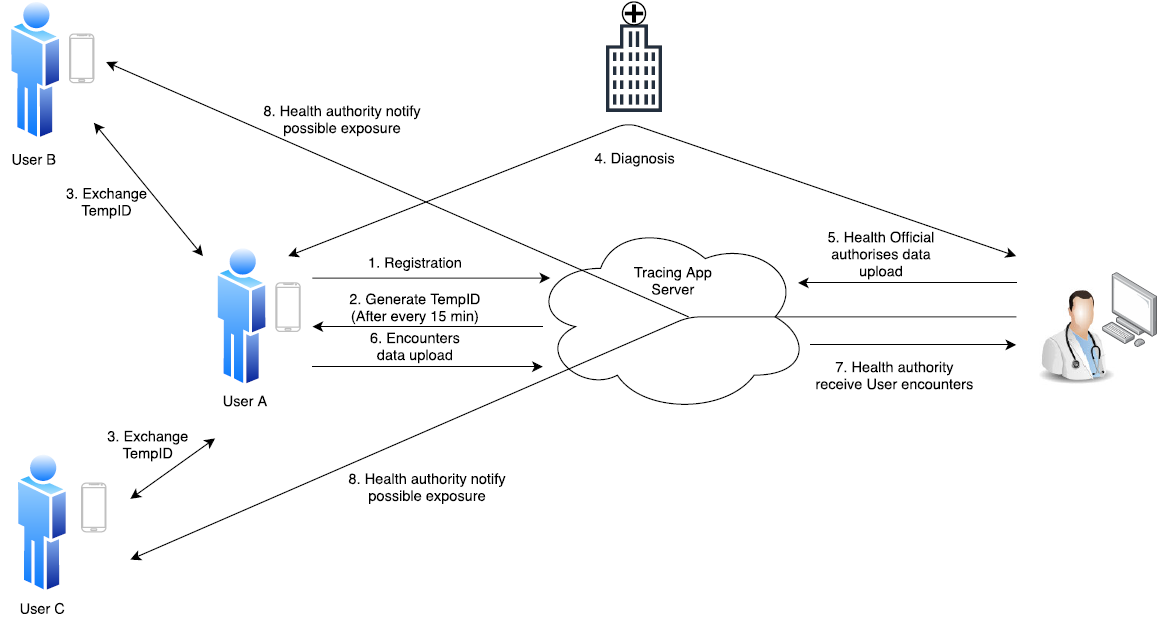
\includegraphics[width=0.8\linewidth]{images/ahmed_centralised.png}

    \caption{ Architecture Overview Diagram for Centralised Architecture from \citet{ahmed_survey_2020}.
    }

    % use the notation fig:name to cross reference a figure
    \label{fig:centralised_arch}
\end{figure}

\subsubsection{Decentralised Architecture:}

Figure \ref{fig:decentralised_arch} shows a decentralised architecture for digital contact tracing. This style of architecture performs the work on the devices, instead of performing it on a central server. The device creates and stores seeds, which are in turn used to create chirps which are short lasting pseudonyms for the device. These chirps are what is exchanged by devices and stored. When a user voluntarily uploads data only the seeds and relevant timestamps are uploaded. Other users can then download the seeds, calculate the chirps, and check if they were exposed.

Counter to the centralised architecture, the decentralised architecture having the majority of the system operations on the mobile device gives this architecture the opposite implications. The privacy is significantly better, no sign-up process is required and the main server knows very little about the users, while decreasing battery efficiency.

\begin{figure}[!htb]
    \centering
    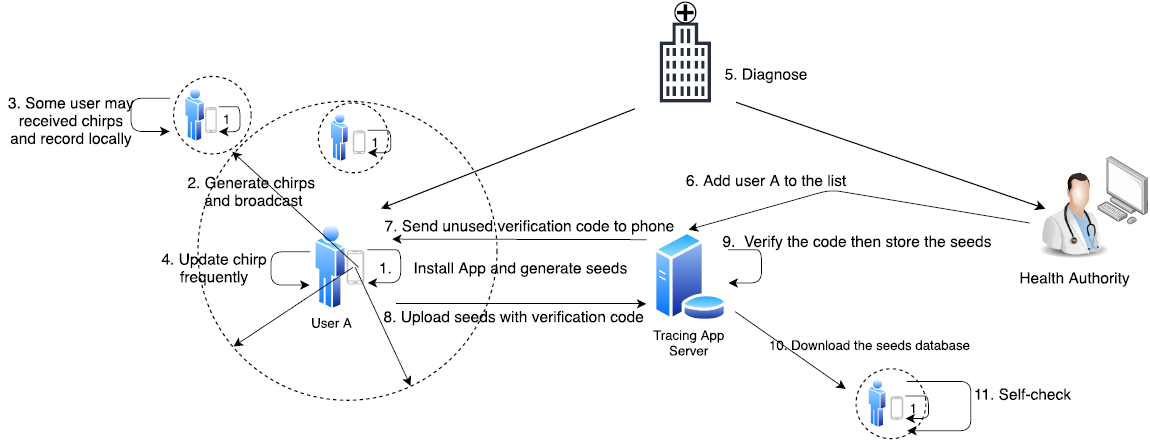
\includegraphics[width=0.8\linewidth]{images/ahmed_decentralised.png}

    \caption{ Architecture Overview Diagram for Decentralised Architecture from \citet{ahmed_survey_2020}.
    }

    % use the notation fig:name to cross reference a figure
    \label{fig:decentralised_arch}
\end{figure}

\subsubsection{Hybrid Architecture:}

The hybrid architecture, Figure \ref{fig:hybrid_arch}, the responsibilities are more evenly split between the client device and the server. Similar to the decentralised architecture the client device handles the generation of "Ephemeral IDs" which are what the devices exchange when a contact occurs. Similar to the centralised architecture the server handles calculating the risk of exposure and the notification of users who may have been exposed.

By nature of its design, the hybrid architecture is intended to compromise the benefits and drawbacks of the centralised and decentralised architecture, Having part of the process on the server allows for better identification of exposure, as it has the whole data-set to perform statistical analysis on. Also, privacy is still preserved with this architecture due to having id creation and management on device.

\begin{figure}[!htb]
    \centering
    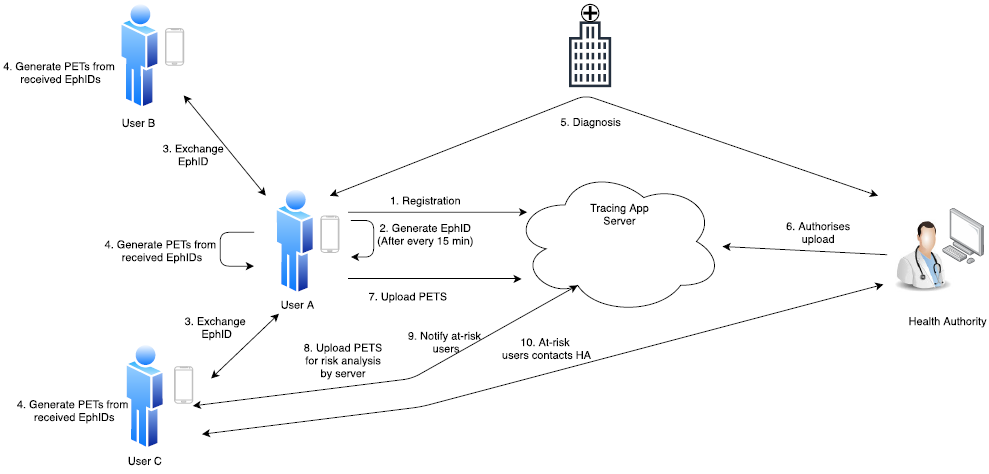
\includegraphics[width=0.8\linewidth]{images/ahmed_hybrid.png}

    \caption{ Architecture Overview Diagram for Hybrid Architecture from \citet{ahmed_survey_2020}.
    }

    % use the notation fig:name to cross reference a figure
    \label{fig:hybrid_arch}
\end{figure}

\section{Bluetooth}

\subsection{Brief Overview of Bluetooth}

Bluetooth, also referred to as Bluetooth Classic, is a wireless communications protocol, and set of specifications, designed for short-range communication between devices. Developed by the Bluetooth Special Interest Group (SIG), this technology specification has been maturing since 1999 and is currently on version 5.0 of the specification which broughy improved data transfer and tighter security. Like all wireless technologies Bluetooth operates on the electromagnetic (EM) spectrum, at a frequency of around 2.4Ghz.

\subsection{Bluetooth vs Bluetooth Low Energy}

Developed as part of the Bluetooth 4.0 specification Bluetooth Low Energy (BLE) was introduced. The primary feature in the design of BLE is its low power consumption, although this comes at the cost of having a significantly reduced throughput \citep{gomez_overview_2012}. Due to this trade-off BLE is suitable for applications that Bluetooth is not, and vice-versa, such as long-term system state monitoring solutions. Bluetooth consumes too much power, as much as 100\% more during peak power draw \citep{iot_lab_classic_2020}, to be used effectively for this.

Like Bluetooth Classic, BLE operates around the 2.4Ghz frequency band on the EM spectrum. BLE has other similarities with Bluetooth Classic, especially the lower layer architecture as seen in Figure \ref{fig:bluetooth_stack_comparison} where the controller, is very similar. They also share the Logical Link Control and Adaptation Protocol (L2CAP) layer in the host segment, which performs data translation between the upper and lower layers. This is where the similarities end.

\begin{figure}[!htb]
    \centering
    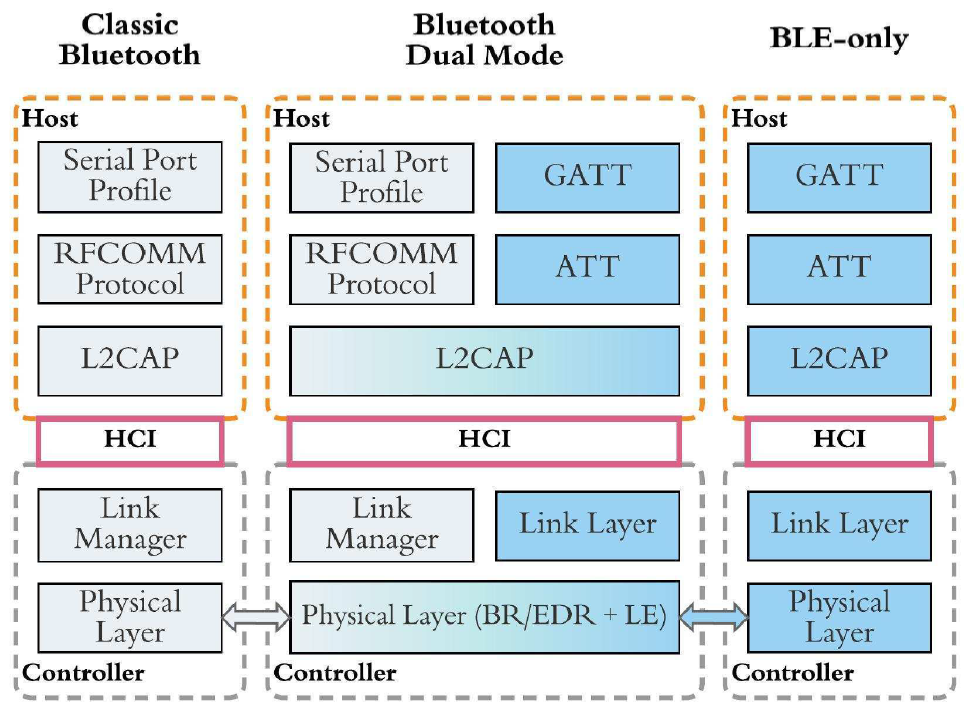
\includegraphics[width=0.8\linewidth]{images/bluetooth_stacks.png}

    \caption{ Comparative diagram of the high level Bluetooth Classic stack vs the BLE stack. The central stack is a "dual-mode" device which supports Bluetooth Classic and BLE \citep{yang_beyond_2020}. }

    % use the notation fig:name to cross reference a figure
    \label{fig:bluetooth_stack_comparison}
\end{figure}

\subsection{Bluetooth Low Energy Technical Stack - High Level}

I will give a brief overview of each layer on the BLE architecture presented in Figure \ref{fig:bluetooth_stack_comparison} from a bottom-up approach.

\subsubsection{Physical Layer:} The physical layer handles the communication hardware with a BLE system. This includes 40 radio frequency (RF) channels which, as previously stated, operate at around 2.4Ghz \citep{yang_beyond_2020}. Of these 40 channels, there are 3 dedicated advertisement channels which allow devices to detect each other and provide the necessary information for establishing a formal connection. The remaining 37 channels are used for data transmission during connections. \citet{gomez_overview_2012} states an important feature of the advertisement channels - they have been selected to mitigate against interference from common IEEE 802.11 channels, a set of standards commonly referred to as Wi-Fi.

\subsubsection{Link Layer:} This layer handles two types of communication connection-less and connection-based. \citet{yang_beyond_2020} describes that when a device only needs to send information to any devices that are listening this mechanism is used. There are two types in this scenario, the advertiser which broadcasts the information, and the scanner which is listening for these broadcasts. This happens over one of the three advertising channels, and devices can simultaneously be advertisers and scanners. Building on this, is connection-based communication. This is used when bidirectional communication is required. Here the advertisement channels are used to present a device as connectable, this is called the peripheral, then for another device to send a Connection Request, called the central \citep{gomez_overview_2012}.

\subsubsection{Host-Controller Interface:} The Host-Controller Interface (HCI) is simply a protocol layer that communicates between the host layers and the controller layers.

\subsubsection{Logical Link Control and Adaptation Protocol:} The L2CAP is held in common with Bluetooth Classic, however the BLE version is both simplified and optimised in order to meet the goals of lower power consumption. The goal is to multiplex the data of the upper layers to run along the link layer, i.e. combine the communication streams of multiple applications for simultaneous transmission \citep{gomez_overview_2012}. The L2CAP packets size is 27 bytes overall, with a 4 byte header leaving 23 bytes for the payload, shown in Figure \ref{fig:l2cap}

\begin{figure}[!htb]
    \centering
    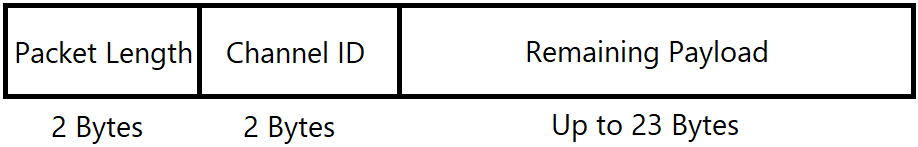
\includegraphics[width=0.8\linewidth]{images/l2cap.png}

    \caption{ Simplified packet diagram for L2CAP packets. }

    % use the notation fig:name to cross reference a figure
    \label{fig:l2cap}
\end{figure}

\subsubsection{ATT:} The attribute protocol sits atop the L2CAP layer, and manages communication between two roles, the client and the server, each of which are on separate devices. The ATT layers manages a set of attributes, this is a data structures which stores the information managed by the above layer, the GATT. An important point is that the two roles are completely separate from the central-peripheral and advertiser-scanner roles \citep{gomez_overview_2012} discussed in the link layer section above. The client can retreive, or write information from an attribute through a direct request to the server. Alternatively, the server can send the client messages in one of two types: notifications and indications. These types are the same bar the aspect where notifications don't require the client to confirm to the server it has receieved the notification. Indications do require this.

\subsubsection{GATT:} The top-level layer in the BLE stack is the genetric attribute protocol. This provides a level of abstraction over the base attributes defined in ATT, descriptors, characteristics, and services. These are linked concepts, a services is made up of characteristics, which in turn optionally contain descriptors. Descriptors provide metadata about the characteristic containing it. Characteristics are pieces of data, containing values and also properties, which act as permissions for what that characteristic allows. Finally, services are a set of related characteristics.

\subsection{Received Signal Strength Indication}

The RSSI is an indication of the reliability of the connection between two devices. \citet{SIG5.0}, in the Bluetooth 5.0 specification, describes how it can be used directly by the BLE protocol for hopping between channels, and can also be accessed by the upper layers of the BLE stack. It also states that if a device supports Received Signal Strength Indicator (RSSI) the accuracy shall be +/- 6 dB, though it should be noted that this varies between hardware implementations. Within BLE the RSSI is an absolute signal strength measurement given in decibel-milliwatts (dBm).

RSSI is commonly used in proximity estimation calculations through the use of a path loss estimation model \citep{ahmed_survey_2020}. However, there are many aspects that can affect the RSSI not just distance. These usually make the signal strength weaker. Examples are: self-interference, material based effects such as reflection and absorption, and noise from other Bluetooth signals.

\section{Background Summary}

\citet{ahmed_survey_2020} presented a survey of the current state of contact tracing as a whole. This helped highlight current methodologies and identified the current implemented methods of using Bluetooth for combatting COVID-19. This allowed for finding the commonalities between this project and existing projects, which in turn provided focus for the novel aspects. There was a heavy focus on privacy concerns; people are more likely to use something they trust. This led to a project focus of inherent privacy by design.

A core commonality between the contact tracing methods I researched, across all papers referenced in the contact tracing section, was the use of Bluetooth. This led to in-depth technical research on Bluetooth, and by extension BLE, using the core specification \citep{SIG5.0} to understand Bluetooth's viability as a distance estimating solution. \citet{gomez_overview_2012} and \citet{yang_beyond_2020} provided much needed additional context to how BLE worked in a more practical sense.

%==================================================================================================================================
\chapter{Analysis \& Requirements}

This chapter discusses the procedure for initial project analysis, and exploratory data analysis to discover specific equation parameters. From the initial analysis, functional and non-functional requirements were gathered. These requirements were created in the initial phase of the project, due to how I structured the requirements there were few modifications made throughout the project lifespan.

\section{Requirements Gathering}

The process followed for requirements gathering was split into 4 stages, each more comprehensive than the last: A high-level mindmap, a set of user personas and stories, some user scenarios, and the requirements themselves.

\subsection{Mindmap}

The first stage of requirements gathering was the creation of a high-level mindmap. This mindmap, Figure \ref{fig:mindmap} was created to map out the initial project space; not everything contained within the mindmap made it further into the requirements gathering process. The mindmap was where the initial thought of having two components, an app on a smartphone and a wearable hardware sensor (ESP32), originated.

\begin{figure}[!htb]
    \centering
    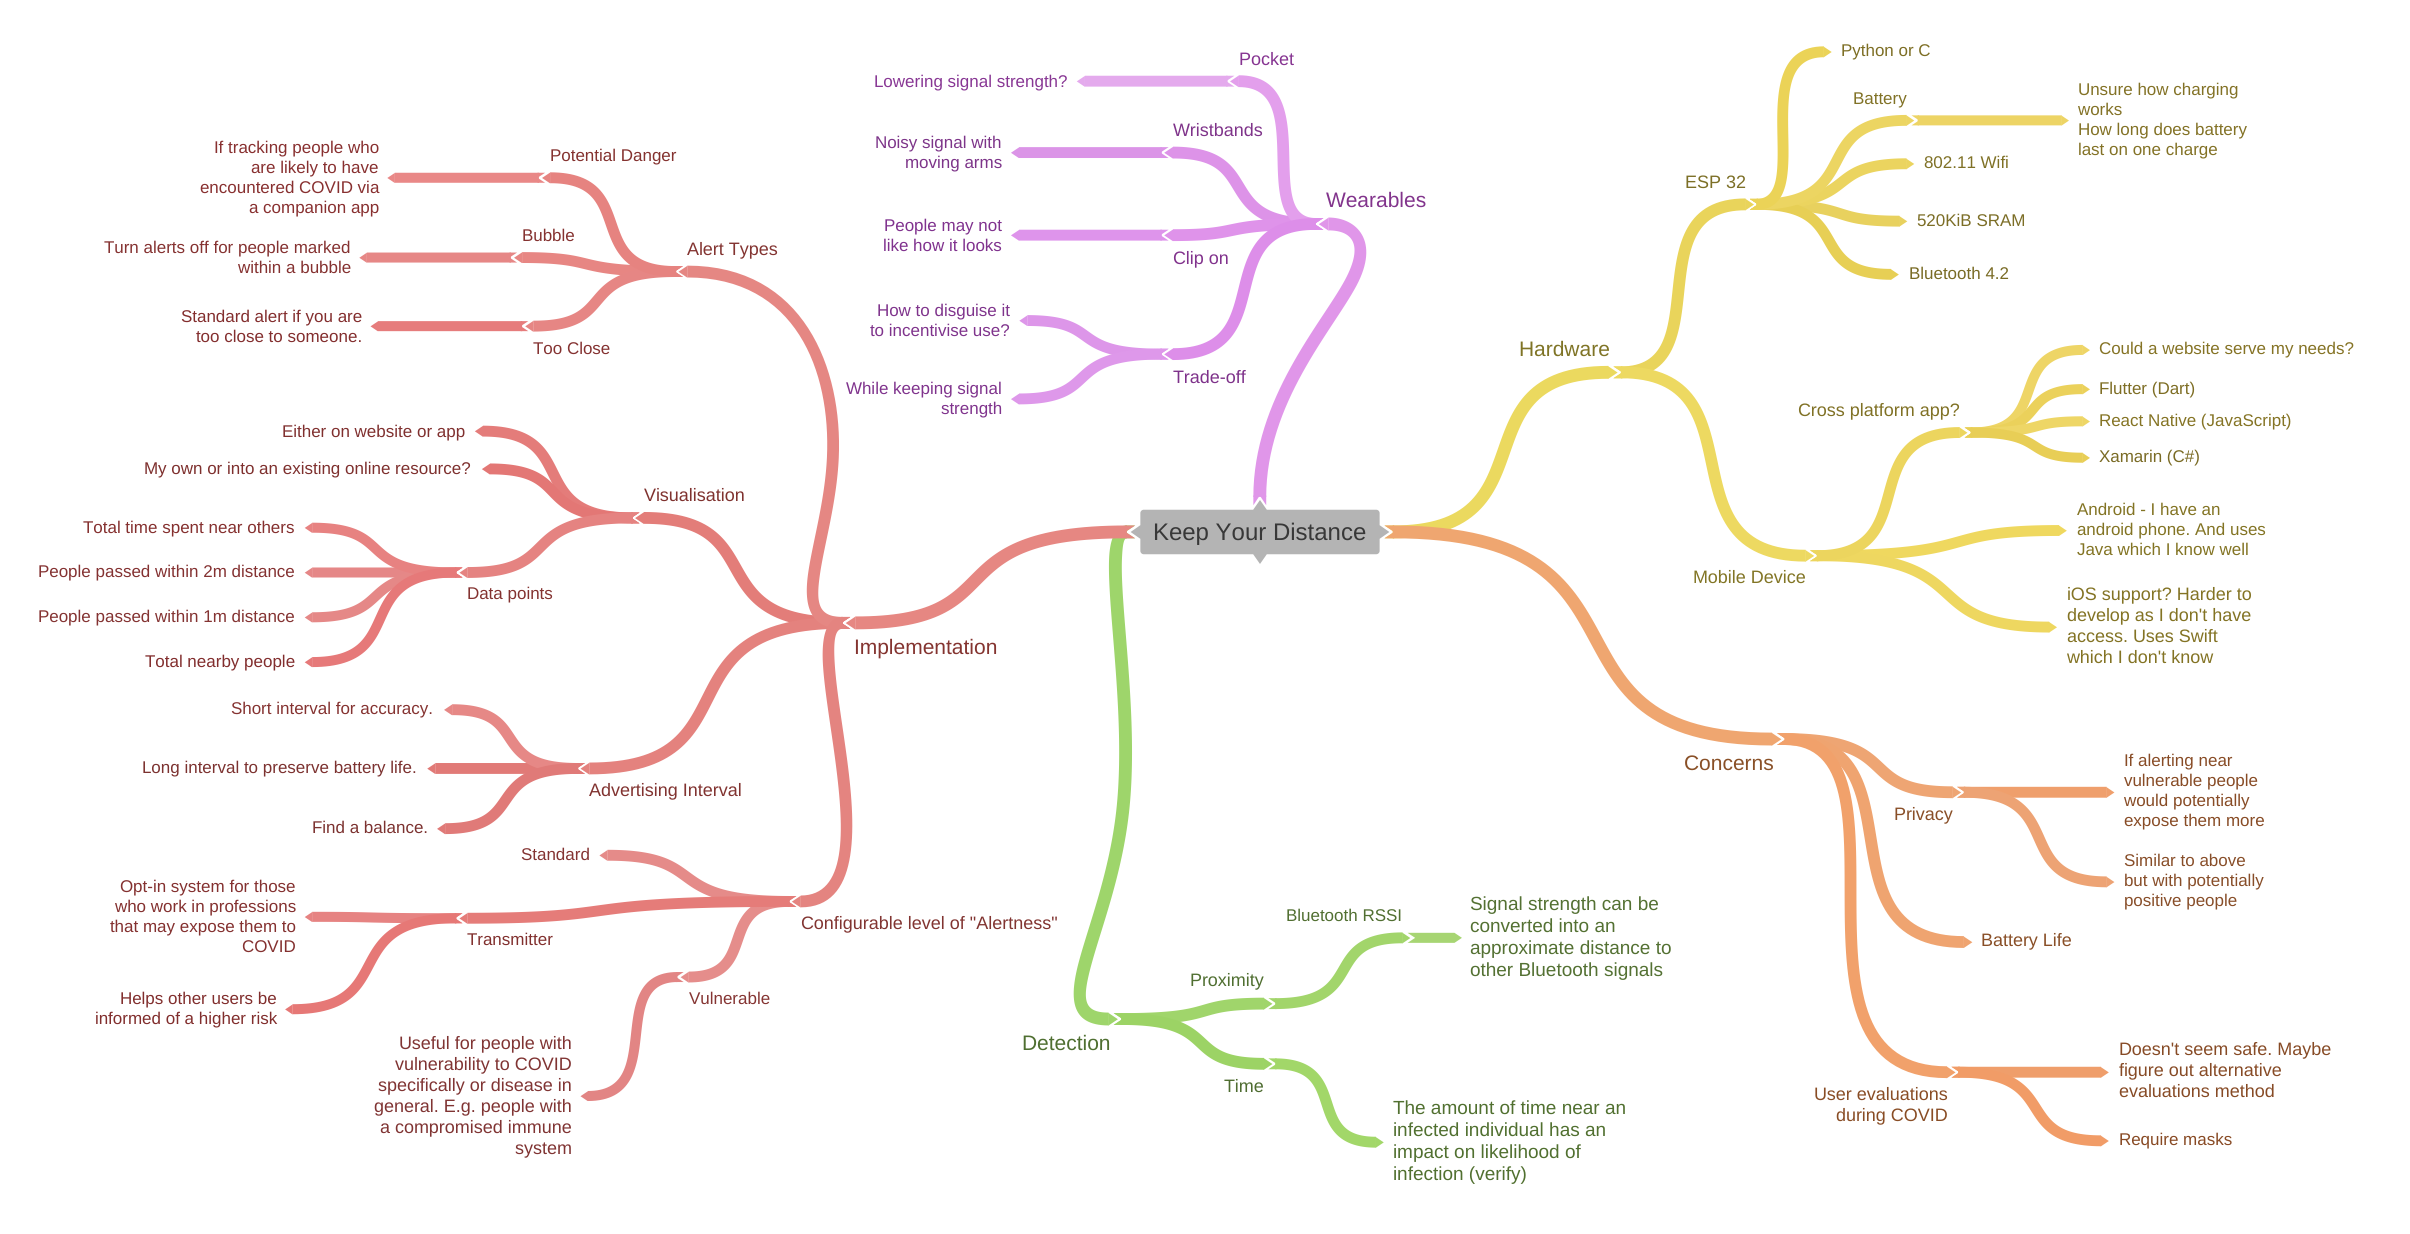
\includegraphics[width=1.0\linewidth]{images/mindmap.png}

    \caption{ High-level mindmap created as first stage of requirements gathering. }

    % use the notation fig:name to cross reference a figure
    \label{fig:mindmap}
\end{figure}

I will briefly summarise the mindmap. The mindmap is composed of five primary themes:
\begin{itemize}
    \item Implementation: Considerations to be made on potential system features such as the visualisations, or the profile system.
    \item Wearables: The initial considered set of ways to wear the device, also includes details in the trade-offs of each option.
    \item Hardware: Looking into the ESP32's hardware and the constraints I would be working with, also details technology options for the project.
    \item Concerns: Details some concerns that the system, or the project, may need to address.
    \item Detection: Examines the factors that are related to covid transmission.
\end{itemize}

\subsection{User Personas \& Stories}

User personas are fictional personalities created during requirements gathering designed to represent a user and identify user needs. User stories make use of these personas to provide a structured view of these needs in an "As, I want, So that" format by using the user persona as context for why those actions are desireable.

Seven user personas, and related user stories, were created during requirements gathering. These covered a variety of user types, considering age, technological literacy, profession, and vulnerability to COVID-19.

The following is an example of a user persona, and related user story:

\textbf{Alex} has a compromised immune system due to chronic illness, this puts them at a much larger degree of risk than the average person from COVID-19. They wish to be able to leave the house more often to have more independence but have to stay more conscious of the people around them.

As Alex, I want to keep a more strict distance from others, so that I don't become infected and become very ill.

\subsection{User Scenarios}

User scenarios utilise the user personas and stories created during the previous stage. They allow for user wants and needs to be further examined by considering a hypothetical situation.

There was a scenario created for each story, seven in total, each scenario considers the steps the user would take to achieve some goal. For each step I considered questions I could not yet answer, ideas that the step had sparked, and general comments on how the step related to the project. For example, in Alex's Scenario (Figure \ref{fig:alex_user_scenario}), I had an idea of making the device detect people based on passive bluetooth signals but determined within the same scenario that this would be out of scope.

\section{Functional Requirements} \label{sec:func_requirements}

The set of functional requirements can be derived once the requirements gathering process is completed. Functional requirements are actions that a user can perform on the system. These requirements were used during the development process to track criteria completion. The MoSCoW prioritisation method \citep{hudaib_requirements_2018} is common way of prioritising requirements. It works by splitting requirements into four categories, each set less important than the last. Must have (M) requirements are the minimal critical set for effective operation. Should have (S) requirements are important but not essential to system operation. Could have (C) requirements are considered nice but the system would still be usable without them. Would be nice to have (W) requirements are requirements that are considered out of scope, and will be discussed towards the end of the dissertation as future work.

\begin{itemize}
    \item \textbf{(M) Real-time RSSI Proximity Sensing: } The device must be capable of sensing another of the same device to within a 2 metre distance. It must be able to do this within three seconds precision.
    \item \textbf{(M) Log data to linked device for visualisation: } Since the device has no on-board storage that survives after power down there is a need to send data to the smartphone over a Bluetooth connection once an interaction has occurred.
    \item \textbf{(M) Visualisations on app: } There should be visualisations and textual statistics on interaction encounters. These should be aimed at informing the user of their current habits and prompting change in necessary.
    \item \textbf{(S) Configurable device: } Allow for configuring device using pre-set profiles. This will need to be synced with the app every time the device boots as it has no power independent storage.
    \item \textbf{(S) Precision in RSSI Proximity Sensing: } The device should be capable of properly differentiating between 1 metre and 2 metre distances.
    \item \textbf{(C) Live visualisation updates on new RSSI value: } Allow for live updating graphs and statistics.
    \item \textbf{(C) Adaptive Advertising Intervals: } This is a battery consideration, a trade-off between battery consumption and advertising frequency. Would work similar on an Additive Increase system, where the interval slowly gets longer and then if it finds another device it resets back to the base interval.
    \item \textbf{(C) Organisation owned devices: } Organisations would have specific configuration tools that would allow data to be sent over Wi-Fi to their servers. The onus would be on the organisation to consider GDPR but the data from the devices would be anonymised.
    \item \textbf{(C) Battery indication on request: } Battery indicator using OLED screen but only when requested by user to preserve battery.
\end{itemize}

\section{Non-Functional Requirements} \label{sec:non_func_requirements}

Non-functional requirements are properties of a system which can be observed by the user. I used the same MoSCoW method the prioritise the non-functional requirements. Similar to the functional requirements, the would like to have non-functional requirements will be discussed as future work.

\begin{itemize}
    \item \textbf{(M) Colour-blind Acessibility: } The system must be usable to colour-blind users.
    \item \textbf{(M) Responsiveness: } The system must be responsive, it should not enter any waiting states.
    \item \textbf{(M) Ease of Use: } The system must be easy to use by a wide range of untrained users.
    \item \textbf{(M) App Design: } The app must follow the recommended guidance on the Android Developer Documentation.
    \item \textbf{(S) Subtle Alert: } The system should be capable of alerting the user and only the user.
    \item \textbf{(C) Organisational Privacy: } The system should not allow the organisation to identify employees from interaction information.
\end{itemize}

\section{Exploratory Data Analysis}

Exploratory data analysis was conducted both in the initial stages of the project and again later in the project with a more finished prototype. The aims of this analysis were to investigate the performance of the ESP32 BLE hardware and to find suitable parameters for calculation of the distance based on RSSI. The exact details of the formula will be discussed in the implementation section, the relevant parameters were the environment factor and the measured power. Exploring this early better informed initial requirement specification, while performing late-stage analysis helped reinforce that the requirements were correctly defined.

The analysis procedure was similar in both the initial analysis and late stage analysis. Starting from 0.5 metres apart and going up in 0.5 metre increments until 2.5 metres 250 rssi values were recorded. The NumPy and Pandas python libraries were used for data processsing, along with MatplotLib and Seaborn being used for data visualisation. A large range of graphs were created including violinplots, swarmplots, histograms, density plots, and line graphs.

The violinplot of RSSI values against specific distances (0.5m - 2.5m) were useful in getting a high level comparative overview on how the RSSI values were clustered, along with how they varied. To allow for easier comparison a density estimation plot was created which allowed for much easier identification of distinct areas along with overlapping areas that may be problematic.

For finding the best parameters a separate dataset was computed for each environment variable value (integers 1 through 4), considering 50 RSSI values from -100 to -50. For each RSSI value the estimated distance was calculated. These datasets were then compared to the real dataset to find the best fit for each environment variable. To then find the best environment variable the standard deviation of the error between the real dataset and each theoretical dataset was calculated. To show this visually a series of linecharts were created to show the error for each distance category, the mean error, and the median error.

\subsection{Initial Analysis}

For the initial analysis data collection the early prototype version didn't have any form of timing system to determine when packets were missed so as workaround I had the receiving device listen every second, and record a dummy value if a packet wasn't received. This initial analysis was particularly important as it showed the project had potential using the ESP32 hardware Figure \ref{fig:initial_density}. A best parameter fit of environment = 3, measure power = -81 was identified, Figure \ref{fig:initial_best_fit}.

\begin{figure}[!htb]
    \centering
    \begin{subfigure}[b]{0.40\textwidth}
        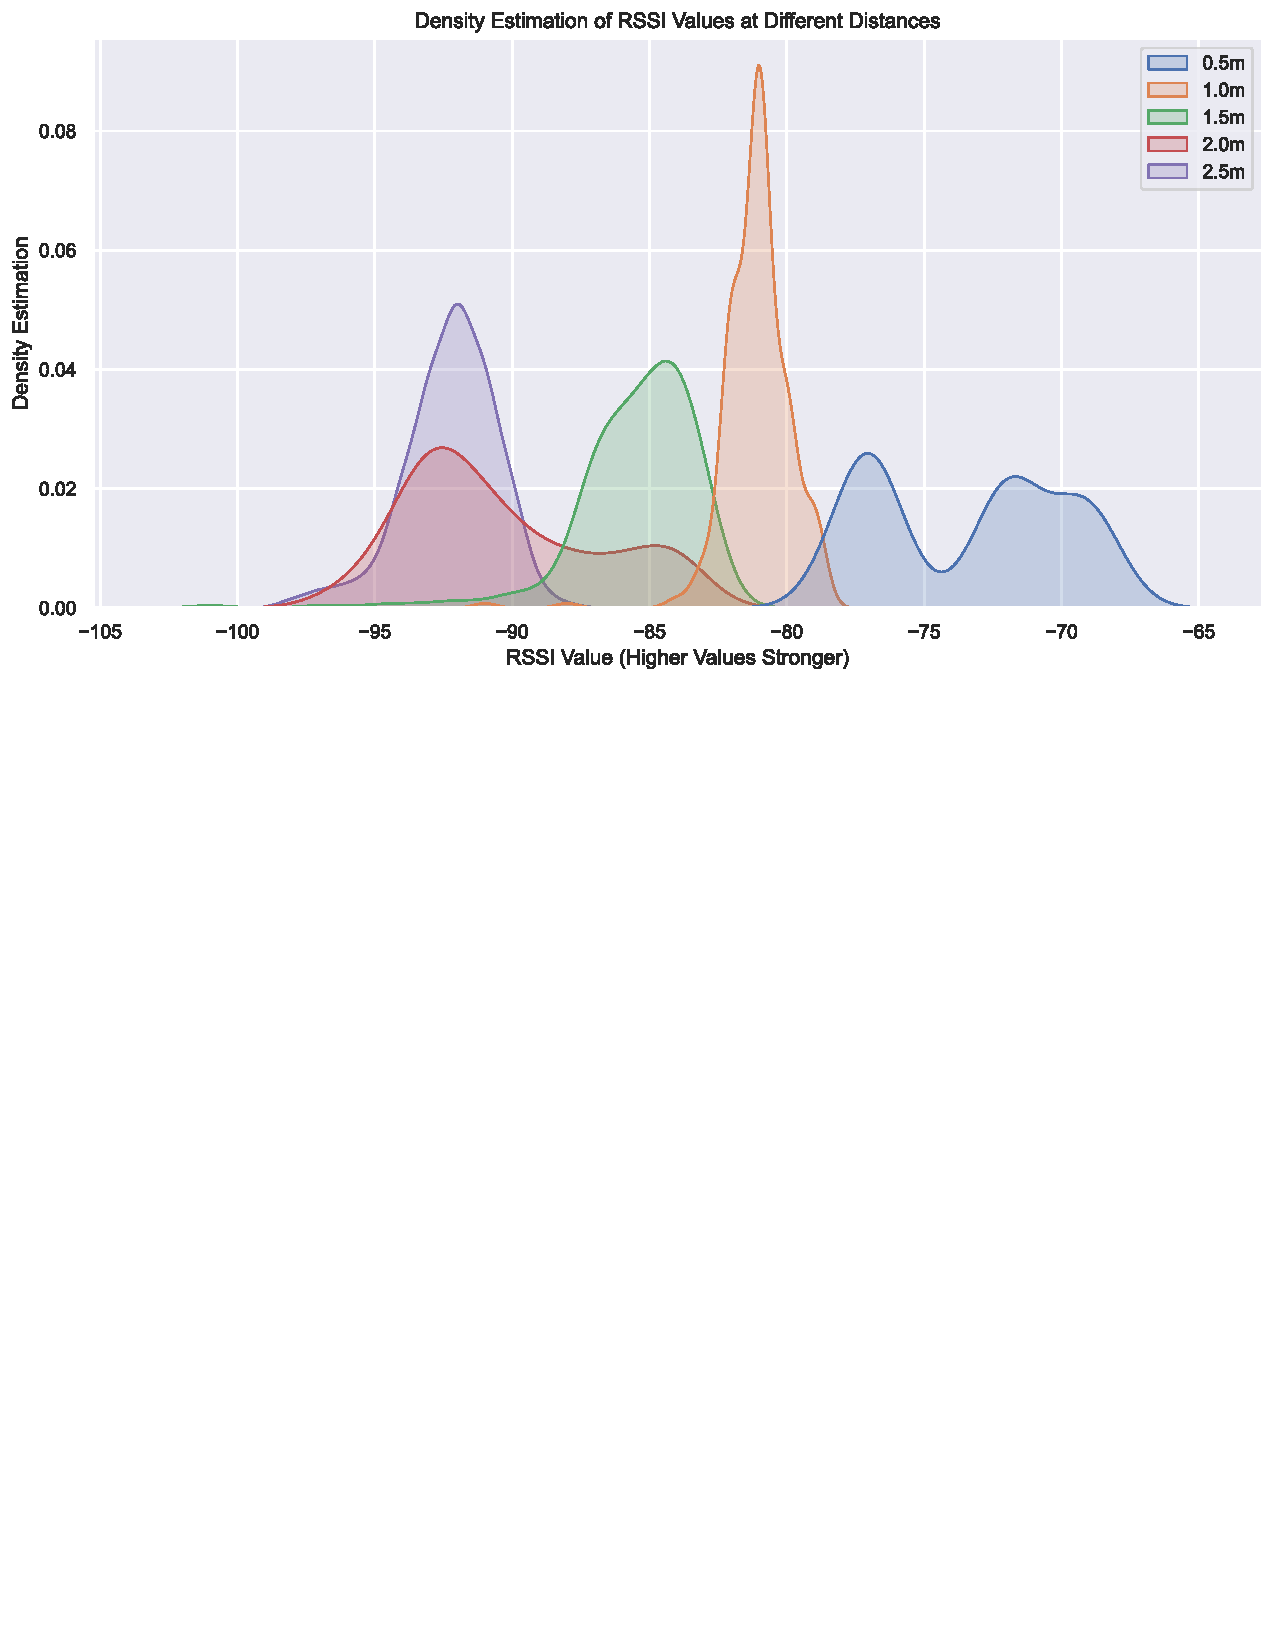
\includegraphics[width=\textwidth]{images/initial_rssi_density.pdf}
        \caption{Density estimation plot for initial exploratory data analysis. Note the distinct peaks for most distances with the exception of red (2.0m) and purple (2.5m).}
        \label{fig:initial_density}
    \end{subfigure}
    ~
    \begin{subfigure}[b]{0.40\textwidth}
        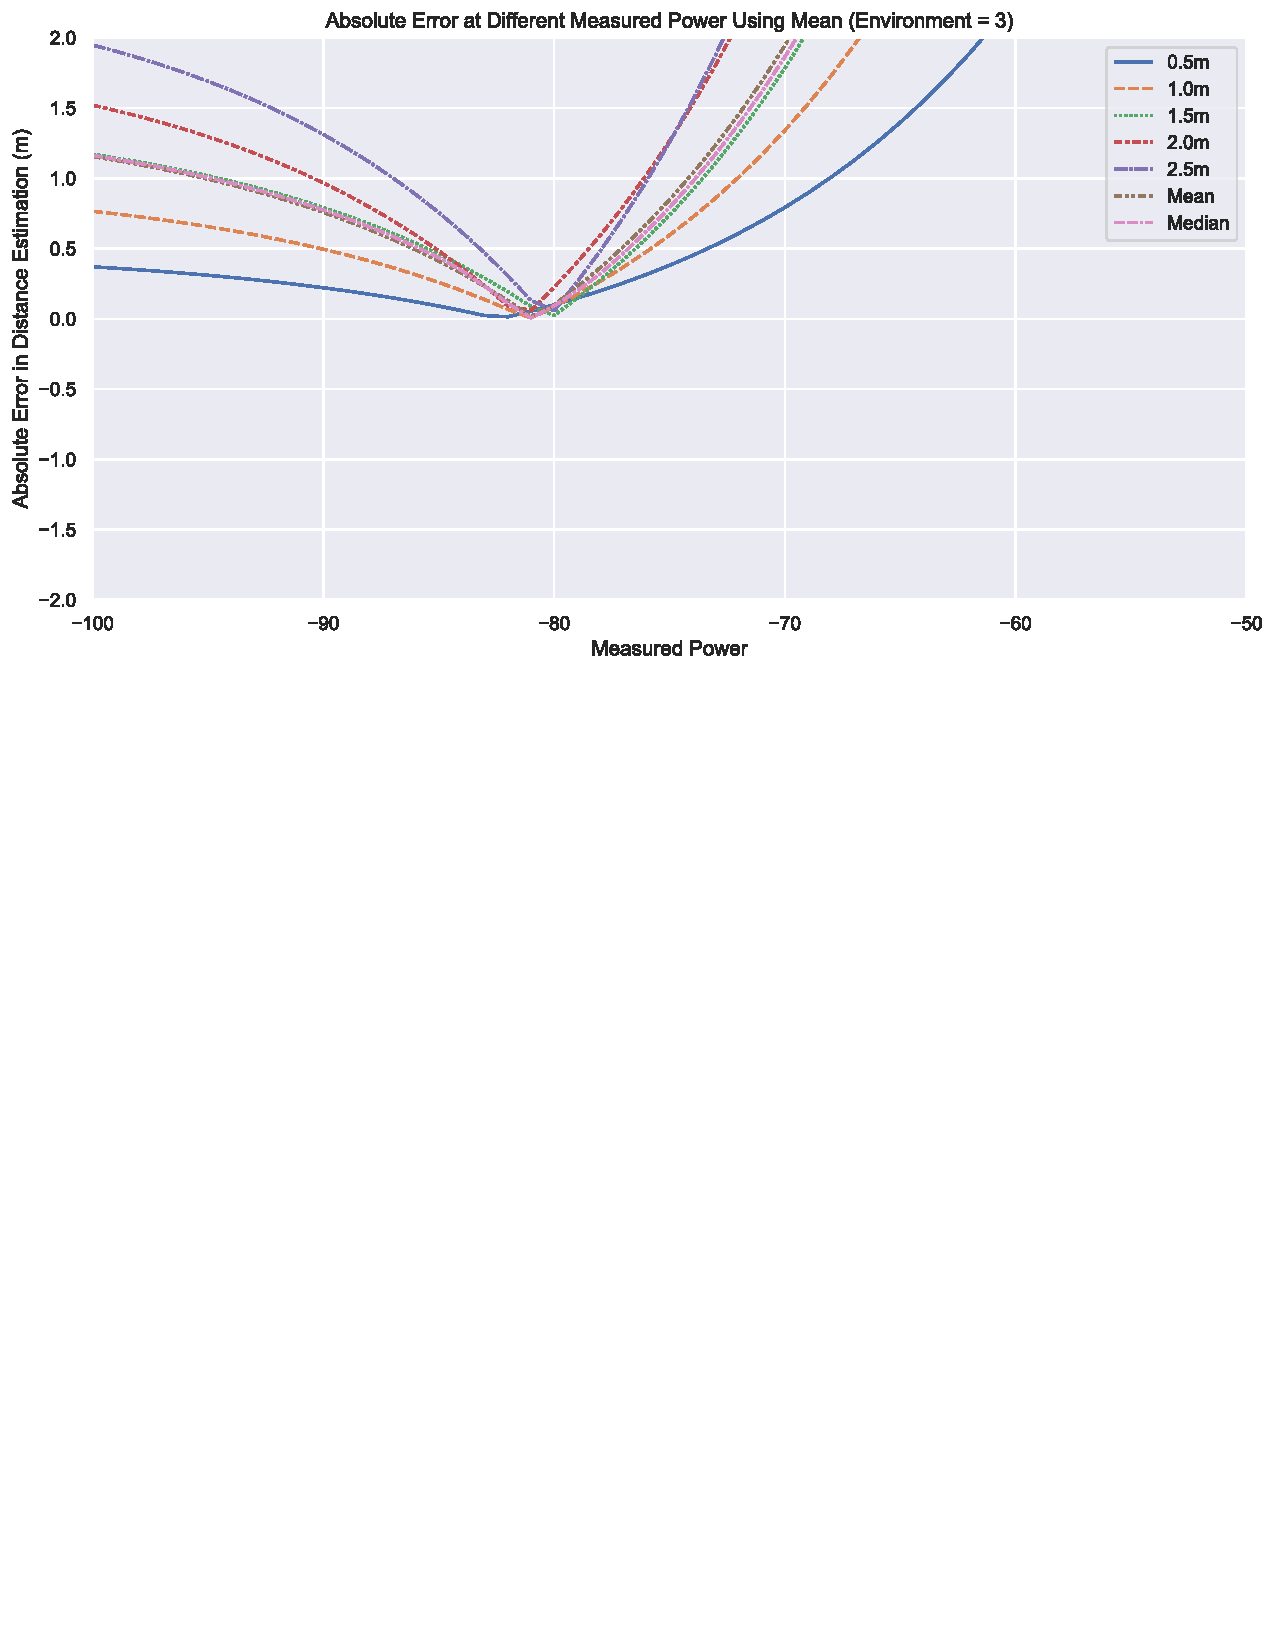
\includegraphics[width=\textwidth]{images/initial_mp_bestfit.pdf}
        \caption{Best fit error plot for initial exploratory data analysis. Graph for environment = 3, shows most common point when measured power = -81.}
        \label{fig:initial_best_fit}
    \end{subfigure}
    ~ %add desired spacing between images, e. g. ~, \quad, \qquad, \hfill etc. 
    %(or a blank line to force the subfigure onto a new line)    
    \caption{ Key plots from initial exploratory data analysis. }
    \label{fig:density_plots}
\end{figure}

\subsection{Late Stage Analysis}

In the late stage analysis the timing system was fully implemented, so I could determine packet loss between packets received. Two types of locations were covered in the late stage analysis: Indoor, and Urban Outdoor. Originally a Remote Outdoor investigation was planned however this was not feasible to set up. For each area the devices were set up in three ways: facing pin side up, facing pin side down, and hanging mid-air facing each other. The aim of this analysis had more of a focus on determining real world performance as opposed to technical feasibility.

After conducting the pin side up and pin side down versions of the indoor experiment and analysing the results, the densities of the distances seemed to have a large amount of overlap Figure \ref{fig:indoor_up_density} - much more than expected, and much more than the initial analysis. The experiment was run again but with a new setup, I had the ESP32s hanging off opposing faces. This allowed for a more realistic scenario as the devices would be facing each other as they would be when worn on people. This yielded closer to the expected result, Figure \ref{fig:indoor_hanging_density}. There was still overlap, however it was clustered into sections. These clusters were 0.5m, 1.0m \& 1.5m, and 2.0m \& 2.5m. Ideally each distance would be separately identifiable as was the case with the initial analysis, however this is still a positive result as it does allow for distinct distance identification.

\begin{figure}[!htb]
    \centering
    \begin{subfigure}[b]{0.45\textwidth}
        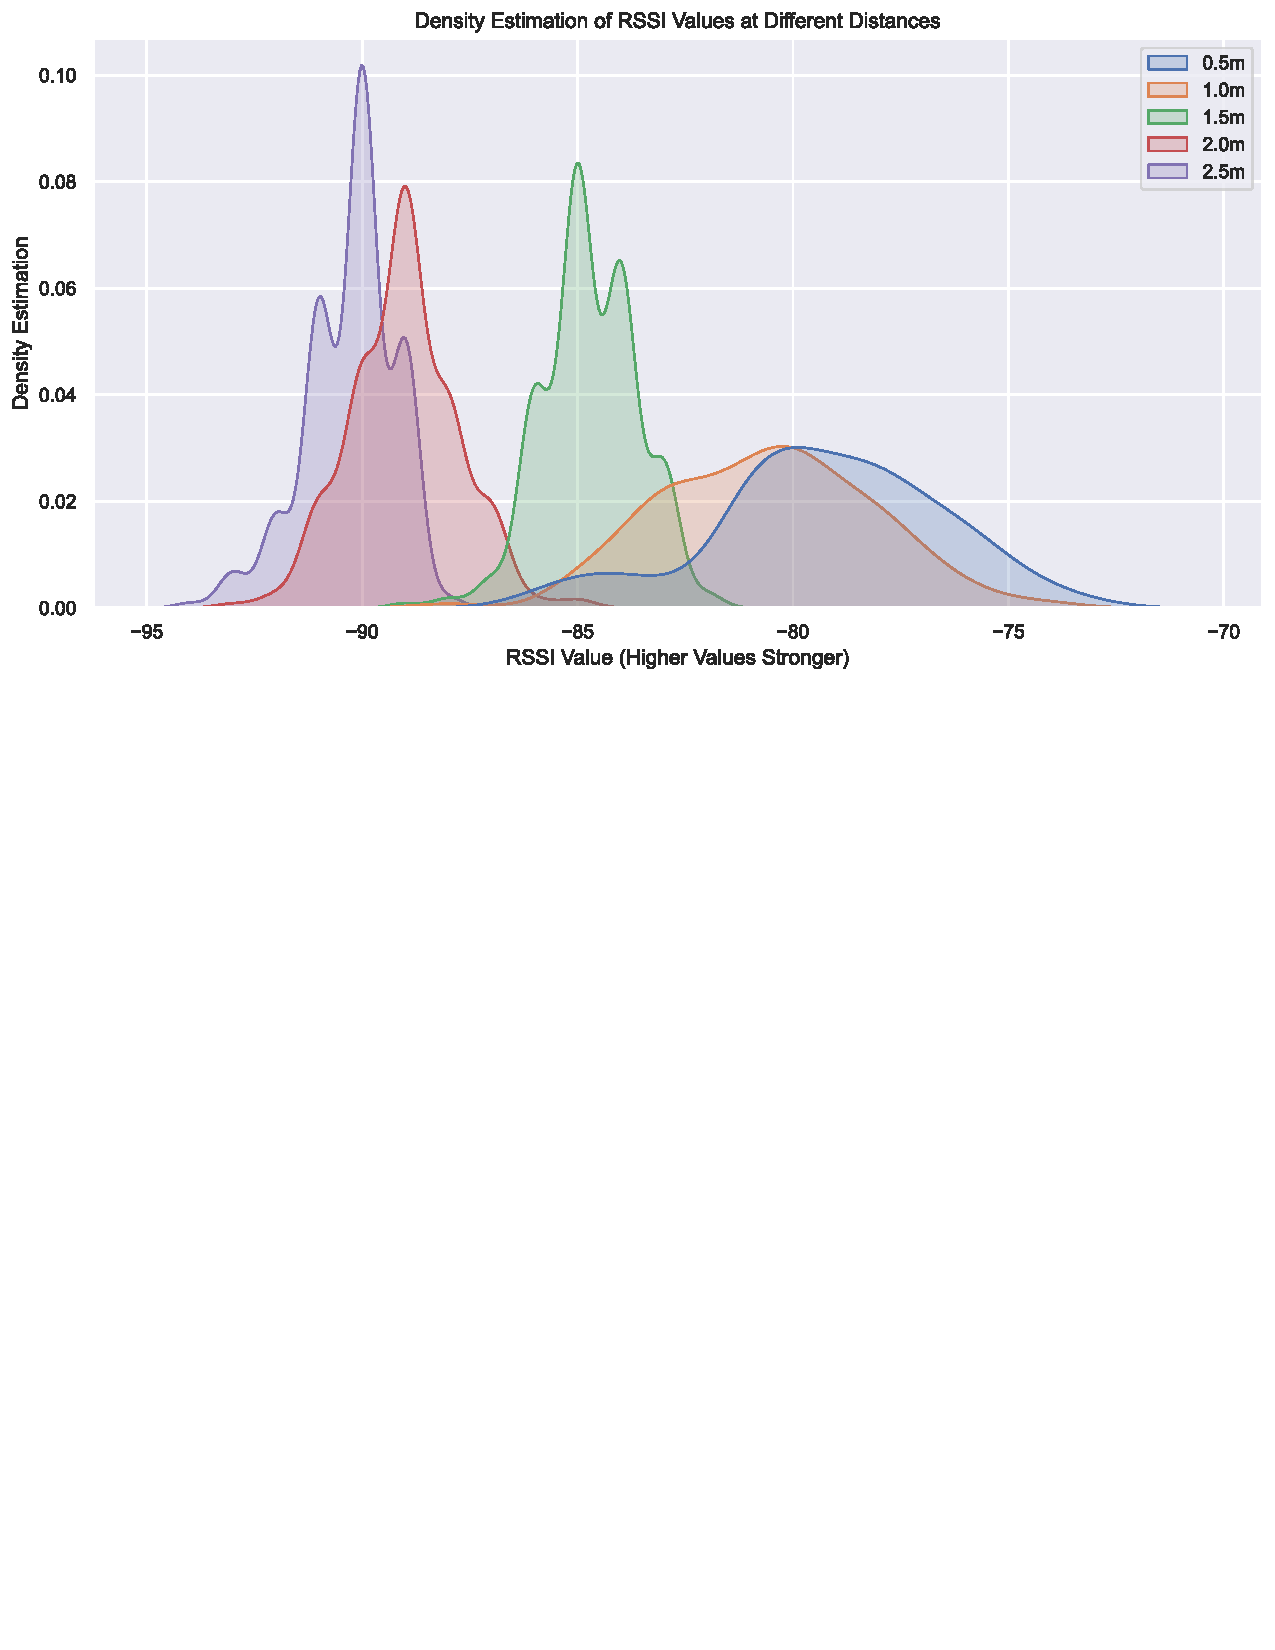
\includegraphics[width=\textwidth]{images/indoor_up_rssi_density.pdf}
        \caption{ Density estimation plot for the indoor pin side up experiment.  }
        \label{fig:indoor_up_density}
    \end{subfigure}
    ~
    \begin{subfigure}[b]{0.45\textwidth}
        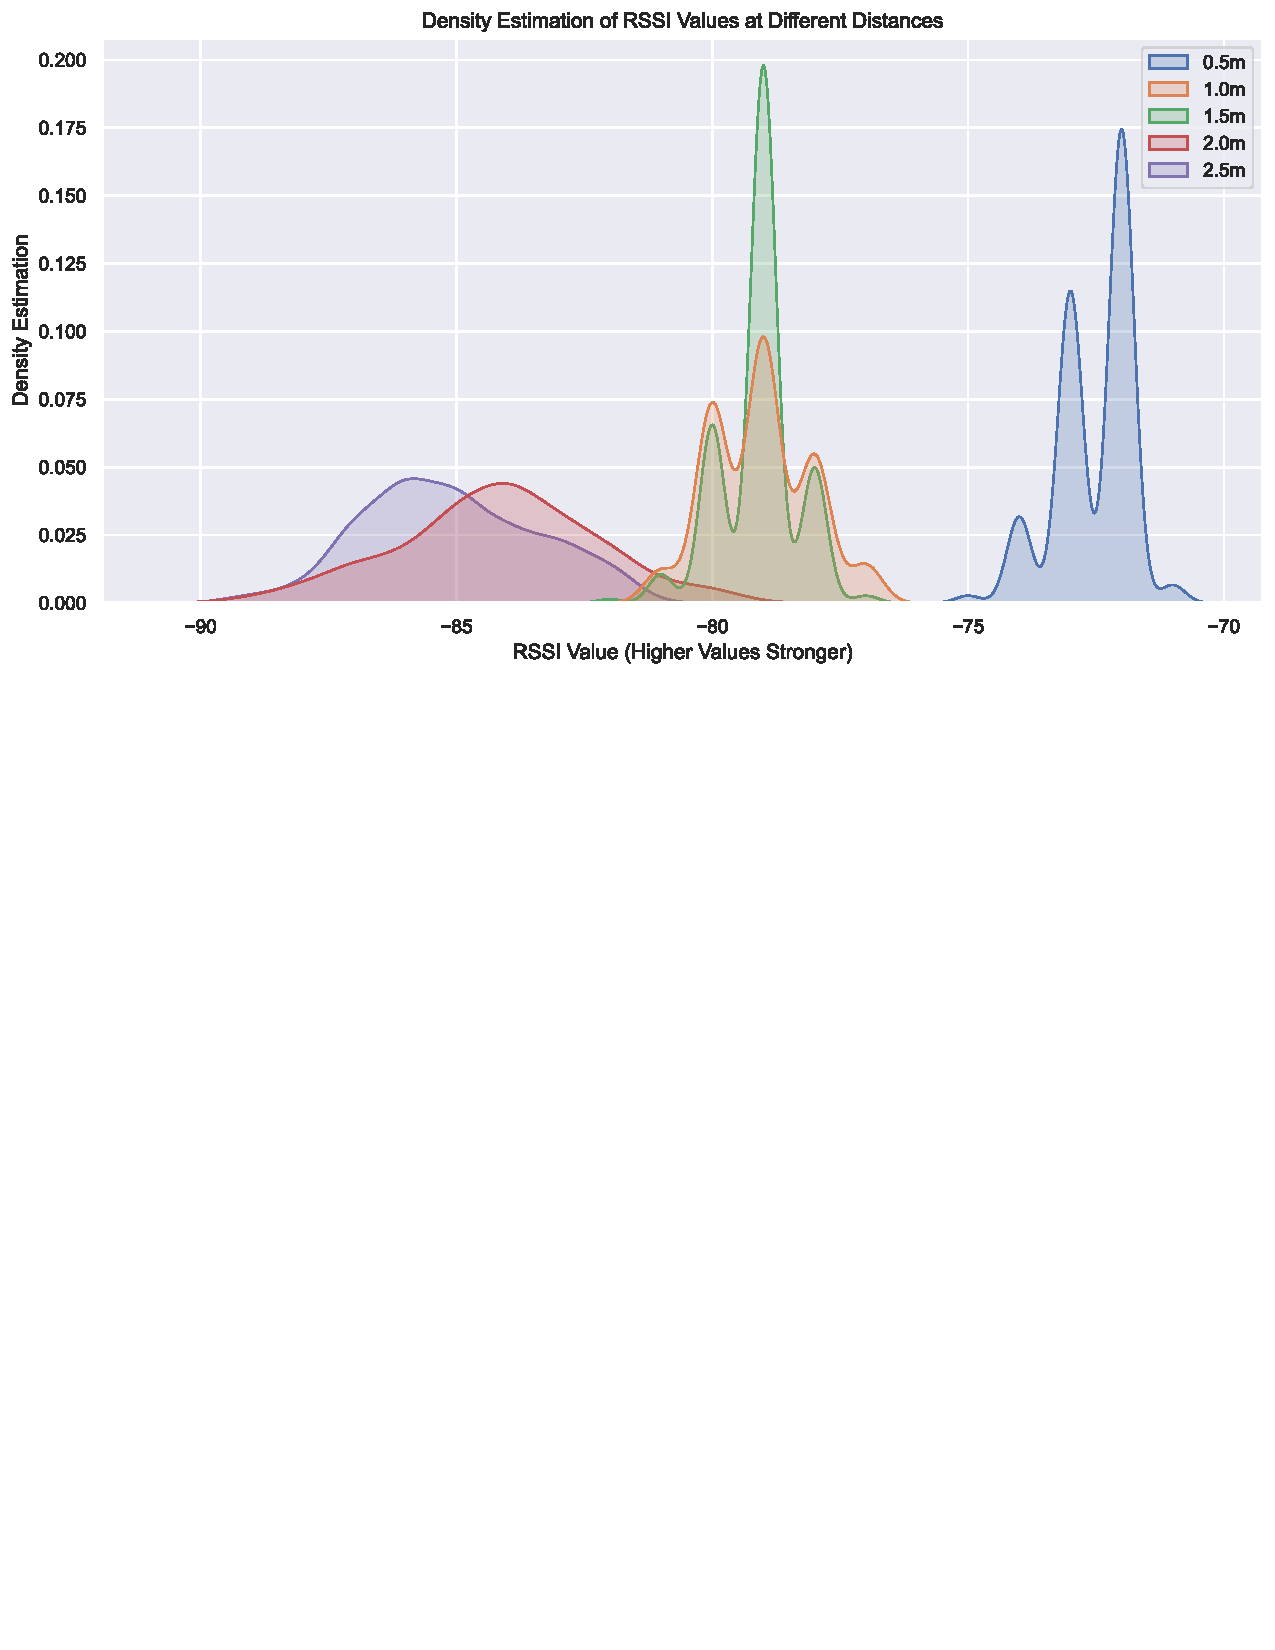
\includegraphics[width=\textwidth]{images/indoor_hanging_rssi_density.pdf}
        \caption{ Density estimation plot for the indoor hanging experiment. }
        \label{fig:indoor_hanging_density}
    \end{subfigure}
    ~ %add desired spacing between images, e. g. ~, \quad, \qquad, \hfill etc. 
    %(or a blank line to force the subfigure onto a new line)    
    \caption{ Comparison of the pin side up experiment density \subref{fig:indoor_up_density} vs the hanging experiment density\subref{fig:indoor_hanging_density} for indoors. The hanging experiment creates more identifiable clusters. }
    \label{fig:initial_plots}
\end{figure}

To ensure fairness between experiments all three variants of the experiment were performed when doing the outdoor experiment. As expected this yielded similar results to the indoor experiment though with somewhat better clustering overall. However, a key drawback to the outdoor conditions was more difficulty in receiving a signal between the two devices; the pin side up variation was unable to get a consistent connection at 2.5 metres. This can be explained when considering the surrounding surfaces. Since waves are reflected off surfaces, when indoors there is more surface area to bounce off and reach the other device.

Since the hanging variant of the experiments is the most realistic in terms of mimicking real world device use, the hanging datasets were used to calculate best fit parameters for the Indoor and Outdoor City profiles. The resulting parameters were very similar with the Indoor, having parameters environment = 2, measured power = -78, Figure \ref{fig:indoor_hanging_bestfit}; Outdoor City was calculated to have the same environment and a measured power of -77, Figure \ref{fig:outdoor_hanging_bestfit}.

\begin{figure}[!htb]
    \centering
    \begin{subfigure}[b]{0.45\textwidth}
        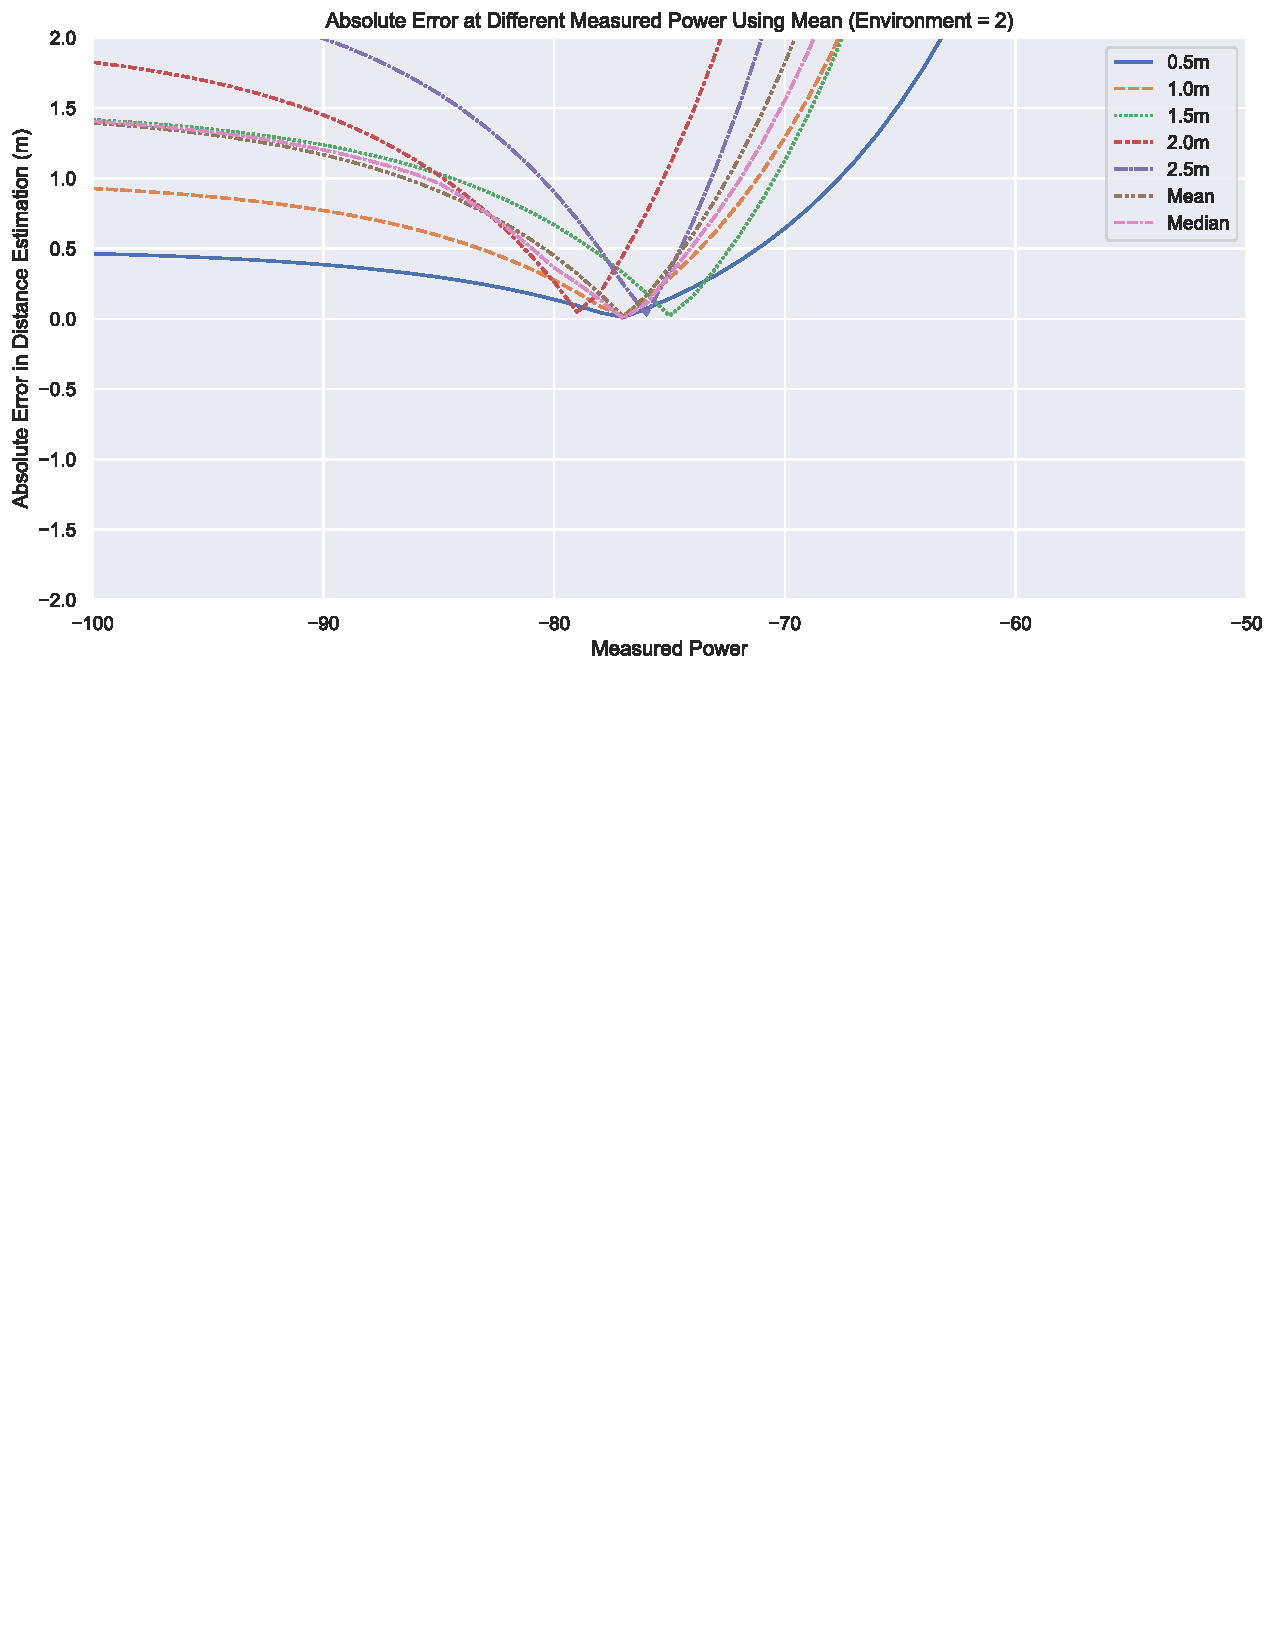
\includegraphics[width=\textwidth]{images/indoor_hanging_bestfit.pdf}
        \caption{ Best-fit graph for the indoor experiment. }
        \label{fig:indoor_hanging_bestfit}
    \end{subfigure}
    ~
    \begin{subfigure}[b]{0.45\textwidth}
        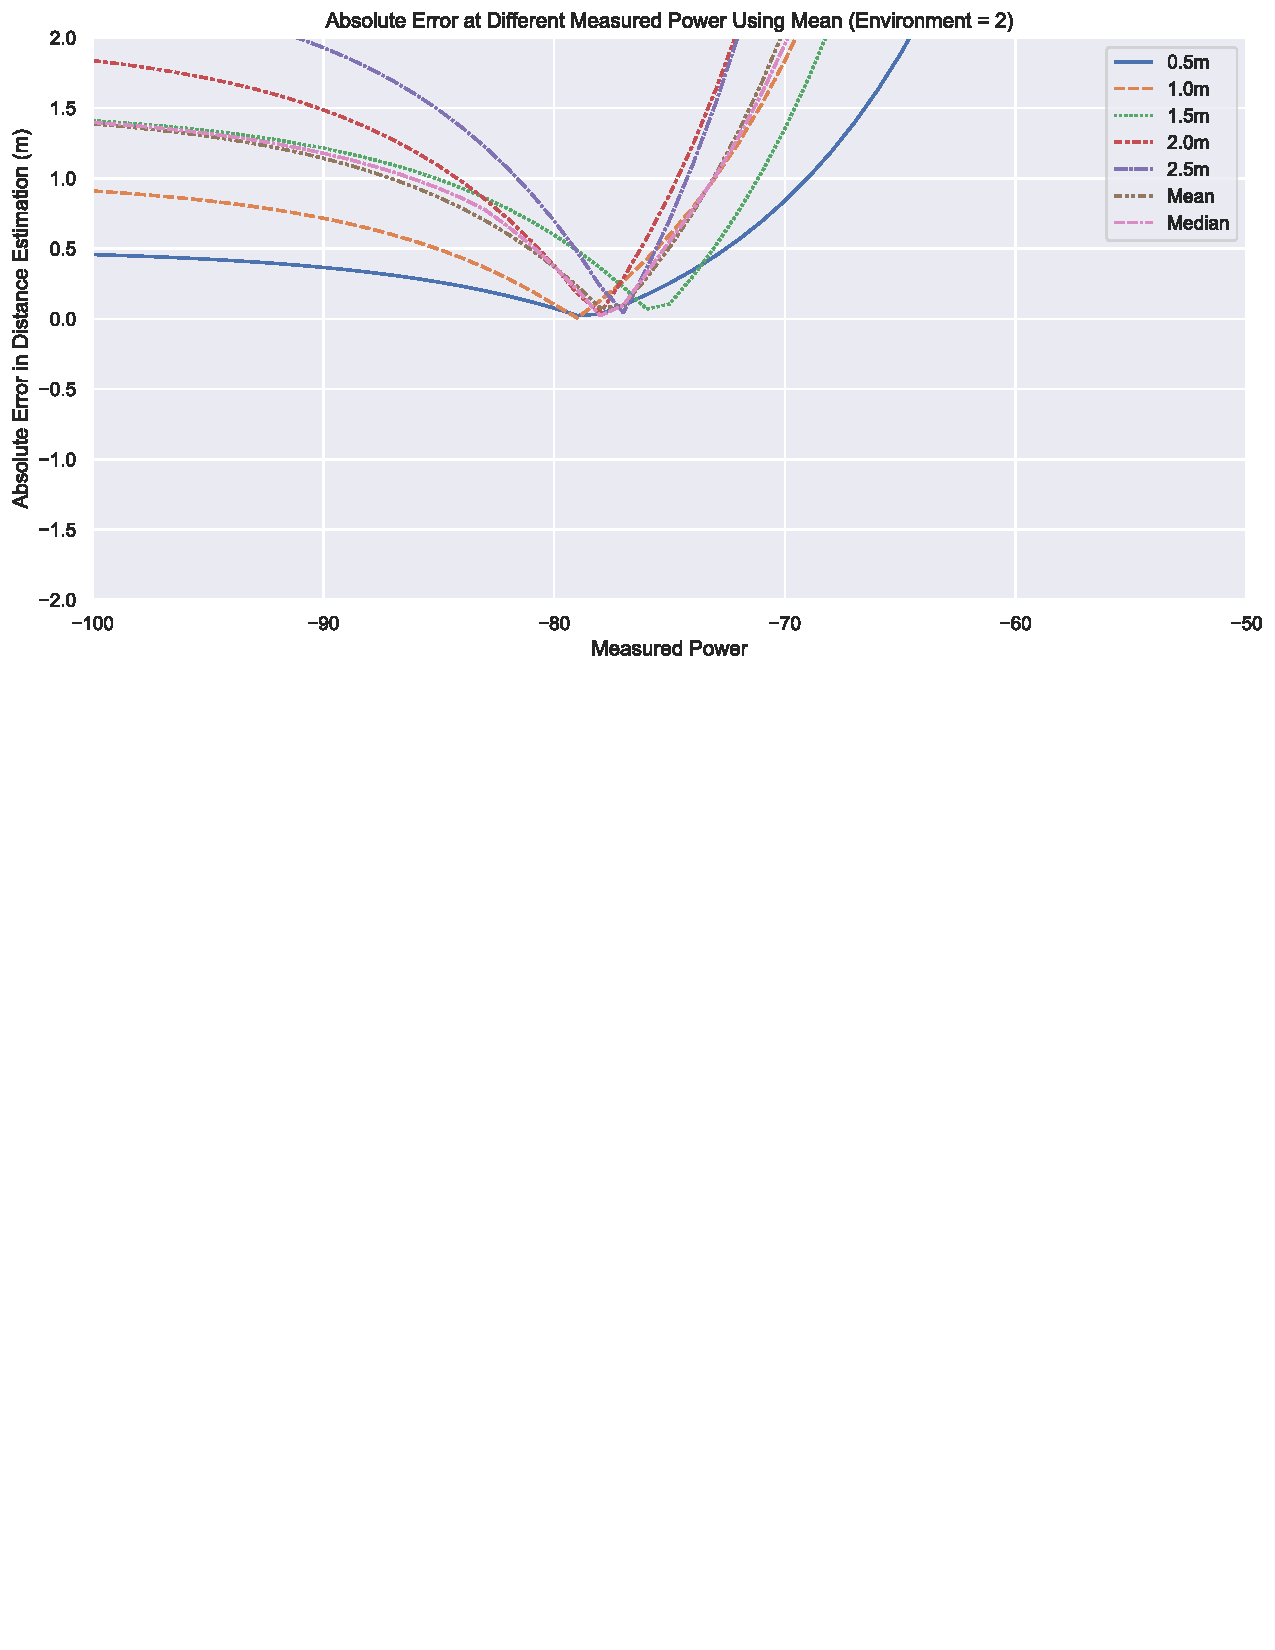
\includegraphics[width=\textwidth]{images/outdoor_hanging_bestfit.pdf}
        \caption{ Best-fit graph for the outdoor experiment. }
        \label{fig:outdoor_hanging_bestfit}
    \end{subfigure}
    ~ %add desired spacing between images, e. g. ~, \quad, \qquad, \hfill etc. 
    %(or a blank line to force the subfigure onto a new line)    
    \caption{ Best-fit graphs based off the hanging experiment variants. }
    \label{fig:bestfit_plots}
\end{figure}

\subsection{Requirements \& Analysis Summary}

The section discussed the requirements gathering process that was used during this project. The MoSCoW prioritisation method was used to allow for a clear set of requirements that had the flexibility to accomodate project changes without having to modify the requirements list. It also discussed how parameter values were identified that could be used during the design and implementation stages.

%==================================================================================================================================
\chapter{Design \& Implementation}

\section{Software Engineering Process}

During the project lifecycle a number of common software engineering practices were employed. The aim was to allow project development to proceed smoothly at an expected pace, while also keeping the project flexible enough that change could occur during the development process.

\subsection{Iterative Developement}

Usually Design and Implementation are discussed separately. However, for this project I followed an agile developement process which used iterative design. A benefit of this is coordinating design and implementation together, which has allowed these to be discussed together in this report.

In iterative development the initial planning and requirements analysis feeds into a cycle, containing: Analysis \& Planning, Design, Implementation, Testing, and Evaluation. Project work was broken into weekly sprints. A sprint is a single iteraton of the cycle to complete a small subset of work. The weekly advisor meeting acted as the end of the sprint, and the beginning of the next sprint, where the produced artefacts could be reviewed. This allowed for the production of sub-system prototypes early in project developement. This was crucial to the timely development of the project as it allowed for errors and incorrect assumptions to be evaluated early so that they did not propogate through the full development of the system.

\subsection{Version Control}

Version control was used extensively, and consistently, throughout the developement of the project. Git was chosen as the version control tool due to its ubiquitous use as an industry standard. GitHub was used to host the repository. This had the advantage of making total project file loss far less likely to occur as GitHub is a large organisation with redundancy in place.

Branching was used during project development when overhauling prototypes developed in previous sprints. These were then merged in with the main branch once tested against the original prototype to attempt to minimise incompatibilities, except where expected. New features were primarily developed on the main branch, as they were not interferring with existing component prototypes.

For this project not only was the code kept on version control, but so to were other project artefacts such as the experimental data and dissertation. The project notes were kept on the GitHub repository under a separate version control using the GitHub wiki feature.

\subsection{Issue Tracking}

To organise tasks, and plan time allocation for a sprint an issue tracker was used. I used a custom Notion board, shown in Figure \ref{fig:issue_tracker}, as opposed to more common issue management system such as GitHub Issues or Trello. This allowed me to integrate project work easily with my existing workflow. Four categories were setup: Not Started, In Progress, Completed, and Constant. These categories indicated the stage that a given issue was at. Each issue could be expanded to provide a projected completion date and a more detailed explanation of the issue. Using this system allowed for effective time management during sprints and provided a clear overview over tasks completed when reviewing the sprint.

\begin{figure}[!htb]
    \centering
    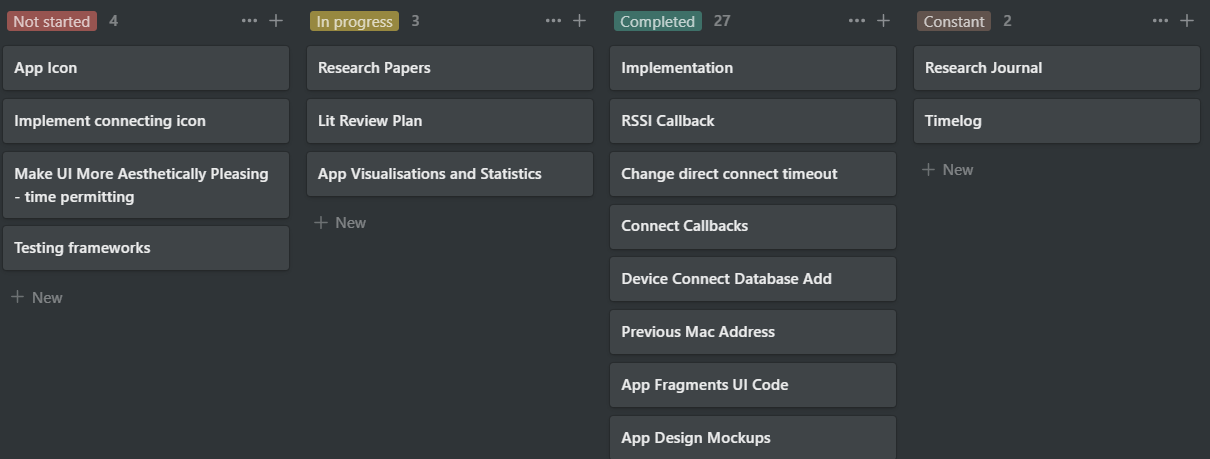
\includegraphics[width=1.0\linewidth]{images/issue_tracker.png}

    \caption{ A custom Notion board used as my project issue tracker. Each colour tag at the top represents a state an issue can be in, the constant issues consist of tasks that must be carried out daily in the project. }

    % use the notation fig:name to cross reference a figure
    \label{fig:issue_tracker}
\end{figure}

\section{Implementation Technology Discussion}

During the early stages of the project, time was spent choosing technologies suited to the project domain. Discussed here are the technologies selected and why they were chosen over other related technologies.

\subsection{ESP32 \& Related Hardware}

The ESP32 is a low-power microcontroller, and was the key component provided by the project specification. It is designed for Ultra-Low power consumption, and low-cost (about £15 for our particular model) making it an ideal choice of hardware for a wearable device. Further, this device has an integrated Bluetooth chip, with support for BLE, meaning that no additional hardware would be needed, as would be required by other microcontroller boards. For this project a specific model, the "Heltec WiFi LoRa 32" \citep{heltec_automation_wifi_nodate}, was used which also contained an on-board LED screen. This screen is the primary notification method. An additional notification method that was added further in development was a vibrotactile motor, used for haptic notification.

\subsection{Platform IO}

Early prototype development on the ESP32 board was done in Micropython, an optimised version of Python 3 designed to run on embedded systems. However, this technology was unsuitable for the project. The documentation for functionality critical to the project, such as BLE, were barebones and the support for BLE was in its early phase. The early prototypes were scrapped and re-implemented in C++ using Platform IO as a build, deployment, and dependency management system. Platform IO has easy integration with the Arduino framework, which contains support for ESP32. The Arduino SDK is a far more mature development environment than Micropython. Further the use of C++ improved code efficiency and made implementation far more structured throughout the project.

\subsection{Android}

When choosing a technology to implement the smartphone functionality there were a number of considerations: the number of users for each Operating System (OS), access to hardware for development and testing, and cost of hardware for the user. Android was the best choice in all cases. First, the market share of Android eclipses that of any other phone OS, with it having an 87\% market share in 2019 \citep{cohen_ios_2020}. Android devices also, on average, cost less the iOS devices; there is much more competition on Android in the entry and mid level smartphone market. iOS was not a feasible option as it requires a Mac for development, which I did not have access to. Finally, cross-platform development using an SDK such as Flutter was considered but ultimately rejected due to the extra complexity that comes with developing a cross-platform app.

\subsection{Java}

The final technology consideration was the programming language to use with the Android SDK. There are two options, Java or Kotlin. Both languages compile down to Java bytecode, and run on the Java Virtual Machine (JVM). Due to this Kotlin and Java can interoperate within a system. Kotlin has a number of advantages over Java. First, Kotlin produces safer code by having nullable and non-nullable types, nullable types come with many restrictions on use which reduce the likelihood of null pointer exceptions. Also, Kotlin has better support for functional programming concepts and reduces the need for boilerplate code, making it more concise.

Even given these advantages Java was still chosen as the language of choice for two reasons: my familiarity with Java as a programming language, and Java has far more documentation online than Kotlin does making solving development issues easier in Java, Java having previously been the standard for Android means that people are likely to have had, and solved, similar issues to the ones I encounter during development.

\subsection{System Architecture}

Now that the initial technologies had been chosen, a high-level system architecture diagram was created, Figure \ref{fig:arch_diagram}. This diagram shows how data and system calls flow between system components, it does not show the specific actions being modelled. The architecture was refined as development progressed and initial assumptions about the system were proven wrong through prototypes, which prompted change. The system architecture was based off two ESP32 devices interacting, however the system theoretically can support more.

\begin{figure}[!htb]
    \centering
    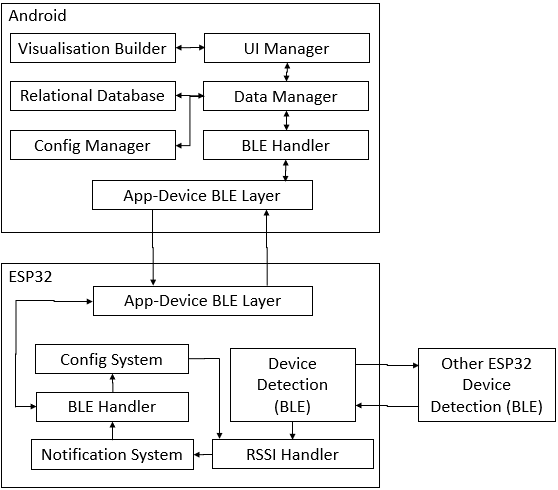
\includegraphics[width=0.5\linewidth]{images/high-level_system_architecture.png}

    \caption{ A high-level system architecture diagram for the Keep-Your-Distance system. }

    % use the notation fig:name to cross reference a figure
    \label{fig:arch_diagram}
\end{figure}

\section{BLE Protocol Design}

As the project developed, a concrete protocol design was created, Figure \ref{fig:protocol_diagram}. This protocol design is the core of the communication between devices and could be implemented on any smartphone - device combination, which allows for the system to be extended in the future. The protocol is split into 4 services. The Device Advertising Service is what allows devices to detect each other. The RSSI service handles the communication of device interaction information to the app. The Heartbeat Service is designed for establishing the connection between the device and app, and reconnection in the case of an interruption. Finally, the Configuration Service allows the smartphone app to configure device settings.

\begin{figure}[!htb]
    \centering
    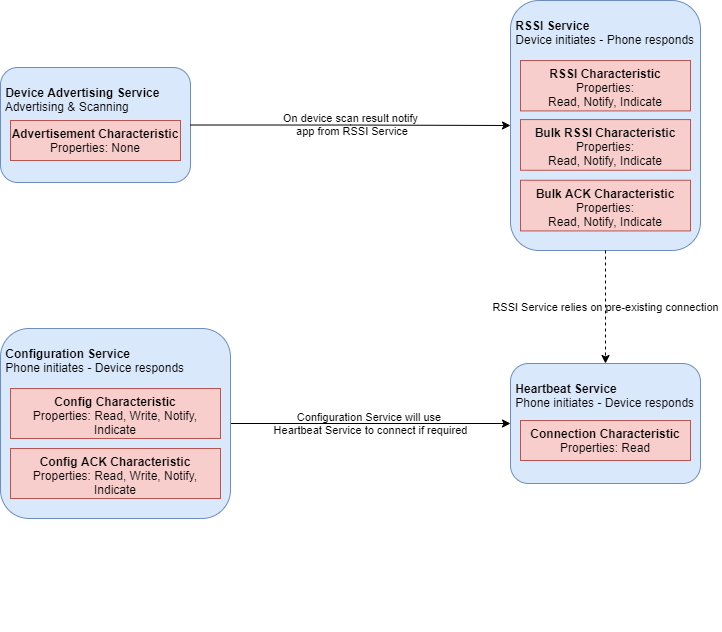
\includegraphics[width=0.8\linewidth]{images/protocol_design.png}

    \caption{ A protocol design diagram. Showing each services components and their interactions. }

    % use the notation fig:name to cross reference a figure
    \label{fig:protocol_diagram}
\end{figure}

\section{ESP 32}

\subsection{Notification System}

The notifications are designed to be simple boolean state objects; there is no variable levels of notification. For this project visual and haptic feedback were designed and explored to notify the user of a social distancing breach. This is the only level of User Interface (UI) on the physical wearable device, so some simple initial sketches were drawn, Figure \ref{fig:device_ui_sketch}. In device code, this was implemented by having an abstraction layer between the separate concrete notification implementations and the function that was exposed to the rest of the system. The state of the system was given to the notification system, which based on configuration activated the physical device hardware. This abstraction allows the notification to be easily extended with new types of notifications, with little modification to existing code.

\begin{figure}[!htb]
    \centering
    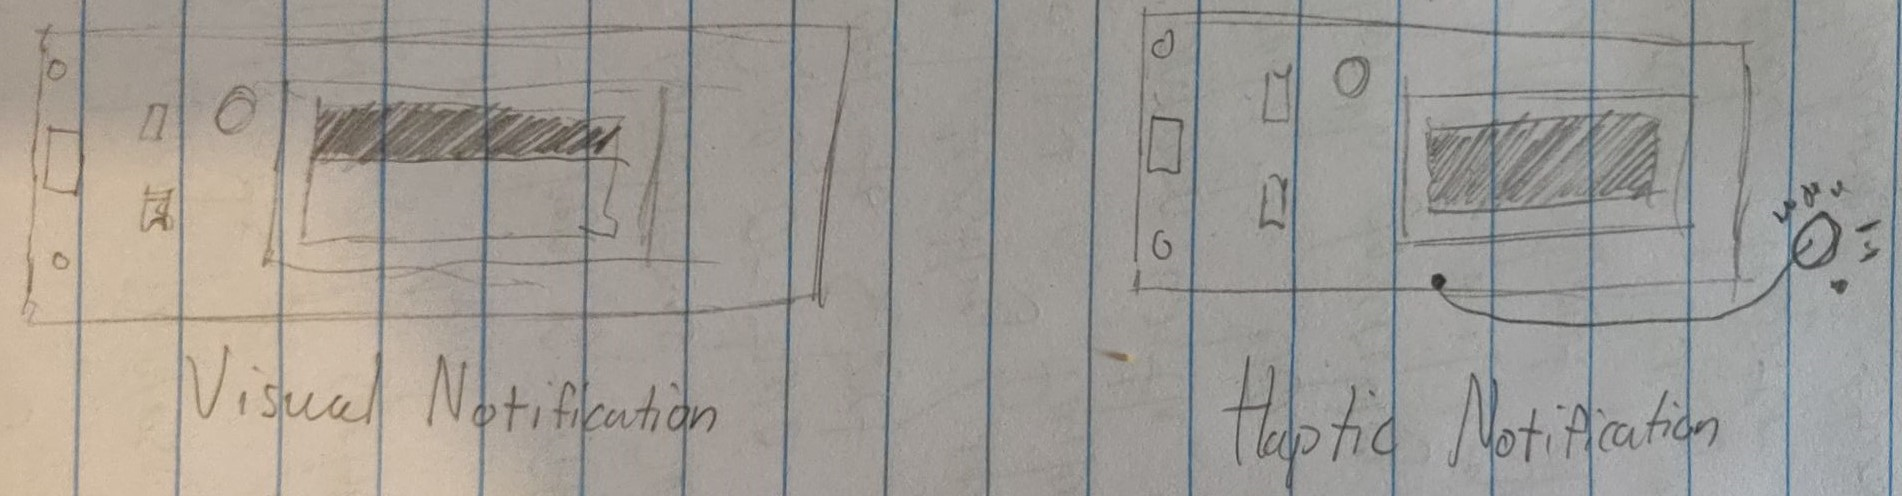
\includegraphics[width=1.0\linewidth]{images/device_ui_sketch.png}

    \caption{ Simple wireframe sketches of device UI. }

    % use the notation fig:name to cross reference a figure
    \label{fig:device_ui_sketch}
\end{figure}

\subsection{Device Detection}

Device detection is done using the connection-less method of BLE communications. Each ESP32 device using this system is simultaneously advertising its existence on the BLE spectrum, while also scanning for other ESP32 devices advertising the same services. As part of this process BLE can determine the RSSI of any other ESP32 devices within its range. A technical constraint of the Arduino ESP32 BLE library is that its scan has a minimum duration of 1 second. This means that there can be a large latency between when an ESP32 first enters the range of another device and when it is detected.

A number of potential ways to interfere with this process were considered, henceforth called interference vectors. These interference vectors are not considered attack vectors, as they don't bear a particular danger to the system users. First, an ESP32 device could be easily faked by duplicating the service IDs and device name. This can't be prevented without making a full-connection which takes longer than the advertisement method, which is unsuitable for use here. However, the only effect of this interference vector is that you would avoid another device, which is not inherently harmful. Similar to this, a high power BLE transmitter could be used which would interfere with the systems ability to detect other devices. This is a real issue, however would only occur in exceptional circumstances due to the cost of specialist high power transmitters. A final interference vector, with a more real use case, is tracking a person using this system. By scanning BLE it is possible to see the device MAC address. A malicious attacker could track the device by looking at the RSSI of the scan and moving in the direction that made it stronger. This risk is difficult to mitigate against, and even exists within existing contact tracing solutions \citep{ahmed_survey_2020}, as even randomising the MAC address wouldn't work due as an attacker would notice when the device changes over and begin to follow this new address. So solving this issue was deemed out of scope for this project.

\subsection{Distance Estimation}

Distance estimation is determined using the RSSI value returned in the device detection phase. This is possible as the signal transmitted by a BLE transmitter decays in strength with distance travelled. To calculate the average RSSI for a given distance $d$ we used a free-space path loss model, Equation \ref{eq:ahmed_formula} from \citep{ahmed_survey_2020}. ${RSSI}_{(d_0)}$ is the measured power which is the average RSSI value, in decibel metres, at the reference distance $d_0$. $n$ is the environmental factor, used in an attempt to capture some of the variation in the environment around the user.

\begin{equation}
    {RSSI(dBm)}={RSSI}_{(d_0)}{(dBm)}-10n\log_{10}{(\frac{d}{d_0})},
    \label{eq:ahmed_formula}
\end{equation}

Since the reference distance in this project is always based off the 1 metre distance Equation \ref{eq:ahmed_formula} can be simplified, for easier and more efficient calculation, shown in Equation \ref{eq:distance_to_rssi}. This is the equation that was used in the final device prototype. The environmental factor and measured power are varied based on the profile selected by the user, then Equation \ref{eq:distance_to_rssi} is used to calculate a threshold RSSI value. This means that only a single calculation needs to be performed on the device when the configuration is updated, then subsequent distance estimation only needs to check whether the RSSI value is above or below the threshold and by how much.

\begin{equation}
    {RSSI(dBm)}={{RSSI}_{(1m)}{(dBm)}} - 10n\log_{10}{(d)},
    \label{eq:distance_to_rssi}
\end{equation}

Early in the development stages rather than using a target RSSI value as above, the distance was calculated at each interaction then compared with a target distance. This was done by rearranging Equation \ref{eq:distance_to_rssi} to give Equation \ref{eq:rssi-to-distance}. As previously mentioned, this approach was problematic; requiring many applications of the forumla causing increased battery usage. However, this did mean the device knew the approximated distance, whereas using the target RSSI system it only knows whether it is above or below the threshold. Ultimately it was decided to use the target RSSI system and move the use of Equation \ref{eq:rssi-to-distance} onto the mobile device, which could handle more calculations with little increase to battery usage. This means that the device needs to send slightly more data over BLE but this is not a problem since it is still within the packet size limit.

\begin{equation}
    {d}=10^{{({{RSSI}_{(1m)}{(dBm)}} - {RSSI(dBm)})} / {10n}},
    \label{eq:rssi-to-distance}
\end{equation}

\subsection{Packets}

Information is sent over the BLE network as a byte stream. The payload has a maximum size of 20 bytes, once bytes attached by the various BLE layers are accounted for. This is a tiny amount of data, so some data trunaction had to take place before and after sending. Data truncation specifically occurs in both the base RSSI packet and the bulk RSSI packet \ref{fig:main_packets}.

Figure \ref{fig:rssi_packet} shows the base RSSI packet. This contains a 12 byte mac address, in string representation form, which is the identifier of the other device found, which is needed for separating encounters. Without the mac address, if there were two other devices the app wouldn't be able to tell these apart and they'd get logged as a single interaction. It also contains a 1 byte RSSI value.

Figure \ref{fig:bulk_packet} shows the extended bulk RSSI packet, that is used when the device is storing interactions in RAM and sending them all at once. To do this a time offset is required, the timestamp is a 4 byte integer of milliseconds since the interaction occurred. This timestamp is sent in little endian form, as this is what the ESP32 uses so not having to perform a conversion saves cycles on the device. The app handles conversion to its native format of big endian. The beginning of the packet is identical to the base RSSI packet.

\begin{figure}[!htb]
    \centering
    \begin{subfigure}[b]{0.8\textwidth}
        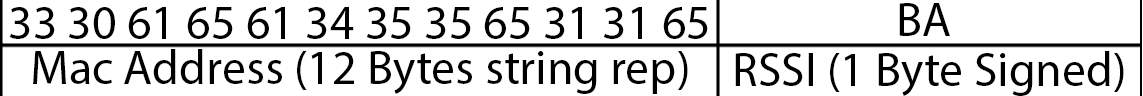
\includegraphics[width=\textwidth]{images/rssi_packet.png}
        \caption{Packet diagram for the base RSSI packet.}
        \label{fig:rssi_packet}
    \end{subfigure}
    ~
    \begin{subfigure}[b]{1.0\textwidth}
        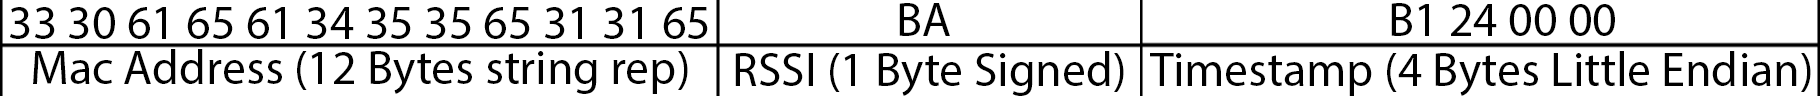
\includegraphics[width=\textwidth]{images/bulk_packet.png}
        \caption{Packet diagram for the extended bulk RSSI packet.}
        \label{fig:bulk_packet}
    \end{subfigure}
    ~
    \caption{ Two packets core to the communication between device and smartphone app. }
    \label{fig:main_packets}
\end{figure}

In the ESP32 BLE library the device mac address is exposed as a string, representing the hex digits of the mac address bytes separated by a colon, e.g. "1A:2B:3C:4D:5E:6F". Sending this would require 17 bytes, which when combined with other packet data would exceed the 20 byte limit. The solution to this was to process the string and remove the colons, as these contributed no information, and could be reconstructed on the app end. Late in the project a function, not included in the documentation, was found that exposed the raw mac address in bytes. This would be the preferred way to send this data, however given time constraints the decision was made not to refactor.

The configuration packets have a separate format, Figure \ref{fig:config_packet}. This packet is sent from the smartphone to the ESP32, and is used to change the on-device parameters used in Equation \ref{eq:distance_to_rssi}. All parameters here are in big endian form, which is standard for transmission over a network known as network byte order, and must be converted by the device to its native format. This is not a problem for battery usage as configuration packets occur infrequently. The conversion algorithm involved bitwise operations and is outlined in Figure \ref{cde:conversion}.

\begin{figure}[!htb]
    \centering
    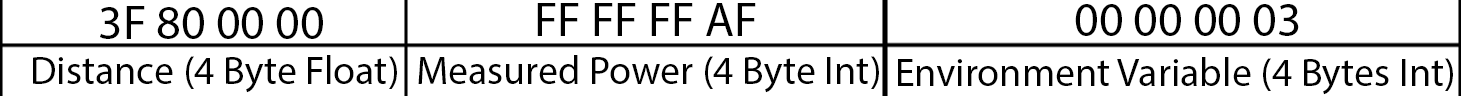
\includegraphics[width=1.0\linewidth]{images/config_packet.png}

    \caption{ Packet diagram for the configuration packet sent from app to device. }

    % use the notation fig:name to cross reference a figure
    \label{fig:config_packet}
\end{figure}

\begin{figure}[!htb]
    \lstinputlisting[language=c, basicstyle=\small]{snippets/endian_conversion.c}
    \caption{ Endianess conversion code from big endian to little endian. }
    \label{cde:conversion}
\end{figure}

\subsection{RSSI Transmission \& Bulk RSSI Storage}

There are two ways interaction data is transferred from device to app. The first, and simpler version is where the phone has a connection open with the device at the time of interaction. In this case the base RSSI packet, Figure \ref{fig:rssi_packet}, is transferred immediately. The second case, where there is no connection between the phone and device is more complex and requires a data structure to store the packet to transfer. The requirements for this data structure were: be able to follow a First In First Out (FIFO) data retrieval pattern, have constant time insertion and deletion, have as little impact on memory footprint as possible, and be able to store up to a set maximum number of items.

I looked at two data structures in particular, a singly linked list, and a circular queue.

A singly linked list consists of nodes containing the data, and pointers to the next node in the list. This has the advantage of only consuming exactly as much memory as it requires, and making it very easy to insert or delete from any positions in the linked list, at the cost of having to traverse the list to that point. However for this case the device would only ever be removing from the head which will always be constant ($O(1)$) time. The downside to the linked list is the overhead of having to store the pointer to the next node alongside the data. These pointers are 4 bytes in size, the data is 17 bytes in size, meaning there is a 23.5\% increase in memory usage which is a scarce resource on the ESP32.

The alternative, and the chosen data structure, is an array-based circular queue \ref{fig:circular_queue}. This works by keeping track of two indexes, a front and rear. The rear index is used to track the most recent element in the queue; when adding to the queue it is added to position rear + 1. The front index keeps track of the oldest item in the queue; when removing from the queue it is removed from position front. This allows the circular queue to wrap around, and fill the queue to capacity, even after some items have been removed.

\begin{figure}[!htb]
    \centering
    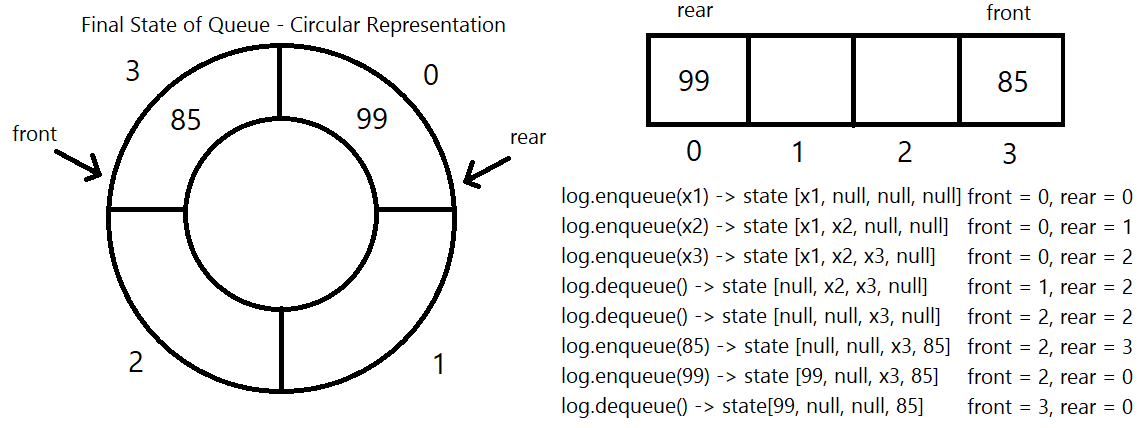
\includegraphics[width=1.0\linewidth]{images/circular_queue.png}

    \caption{ Simple example to explain a circular queue. The key aspect is that the queue can wrap around if there is space in the front of the array and it has reached the end. }

    % use the notation fig:name to cross reference a figure
    \label{fig:circular_queue}
\end{figure}

Since the circular queue is array-based it has a set size, meaning that a maximum size has to be defined and that block of memory set aside. While this sounds like a downside, it is actually a positive; if memory consumption grew unchecked the device would run out of memory. The other primary advantage of the circular queue is that the overhead is constant, only two 4 byte indexing integers are required, so the increase in memory usage can be considered negligible. For this application the circular queue didn't have any downsides, so was implemented.

The queue size was set to be 3000, due to the hardware contraint of limited RAM. With some tweaking this size could be increased, but not by a large amount. At 3000 entries, 17 bytes each, this uses around 10\% of RAM (51kb of 520kb). At 1 value stored per second (the maximum rate for a single device-device connection) this can store 50 minutes of data. However, when multiple devices are being interacted with this time decreases; with 2 other devices 25 minutes, with 4 other devices 12.5 minutes, etc.

Once the phone reconnects to the device it begins transferring from the queue until the queue is empty. It transfers a single packet at a time, only transmitting each packet after receiving an acknowledgement from the app. Note, it does not enter a waiting state here as this is done using the BLE callback functions within the BLE library.

\subsection{RSSI Averaging System}

The RSSI values reported through the advertising packets in BLE are volatile; without either device moving, a wide range of RSSI values can be reported. This means that it is common for devices to switch between being too close, and enough of a distance away, even without moving. This is problematic behaviour; it would be confusing to the user. To solve this a form of averaging is used, to smooth the erratic values and minimise rapid change between the two states.

First two smoothing algorithms were considered: exponential moving average, and sliding window average. The exponential moving average works by weighting the previous values as a new one is considered using Equation \ref{eq:ema}, where w is the weight. The weight is calculated using Equation \ref{eq:weight}, where sf is the smoothing factor, which for this project is 2.0, and m is the number of values to consider.

\begin{equation}
    {RSSI}_{Average}={({RSSI}_{New} * w)} + {({RSSI}_{PrevAverage} * (1 - w))},
    \label{eq:ema}
\end{equation}

\begin{equation}
    w=\frac{sf}{m + 1},
    \label{eq:weight}
\end{equation}

The sliding window average algorithm stores and averages the last n values, this would require $O(nd)$ memory, where $n$ is the number of values to consider and $d$ is the number of devices encountered. The exponential moving average was chosen as the algorithm for the system due to its smaller memory footprint. Since it only requires a single number to be stored it required $O(d)$ space, lower than the $O(nd)$ space that the sliding window requires.

To perform this averaging a data structure was needed that supported: Quick searching to find a given mac address, efficient and consistent insertion and deletion operations, and ideally a low memory footprint. The following were considered: array of structs, sorted array of structs, hashmap, and a red-black tree. The array of structs, could not be easily indexed by mac address so search time would be $O(d)$ which is too slow. The sorted array of structs could be searched in $O(\log{d})$ using binary search but suffered from $O(d\log{d})$ insertion, which was too slow as there would be many insertions. The hashmap has constant time for insertion, deletion, and search. However, it suffers from being an amortised constant time, meaning this is on average; in a worse-case scenario the hashmap could become $O(d)$ for all these operations, so was deemed unsuitabe. Finally, the red-black tree is guaranteed $O(\log{d})$ for insertion, deletion, and lookup; this comes at the cost of an increased memory footprint, and a slower average time complexity than the hashmap but this trade-off was acceptable.

First, the node struct for the tree had to be defined. As seen in Figure \ref{fig:tree_node}, the node is grouped into 3 sections. The data group contains the actual data that we wish to store within the tree. The pointers group contains the related pointers to nearby nodes - this is how the tree is linked together. Finally, the properties group only contains a boolean to set the colour of the node, either red or black. In theory each node should be 29 bytes in total, however, in real hardware implementation the size will be dependant on how the architecture pads the struct. For the ESP32 this is 32 bytes as it pads the single byte boolean out to the nearest 4th byte. This node could be optimised to 28 bytes per node by storing the colour information in the least significant bit of the parent pointer \citep{munoz_bannalia_2008}; this was not implemented due to time constraints.

\begin{figure}[!htb]
    \centering
    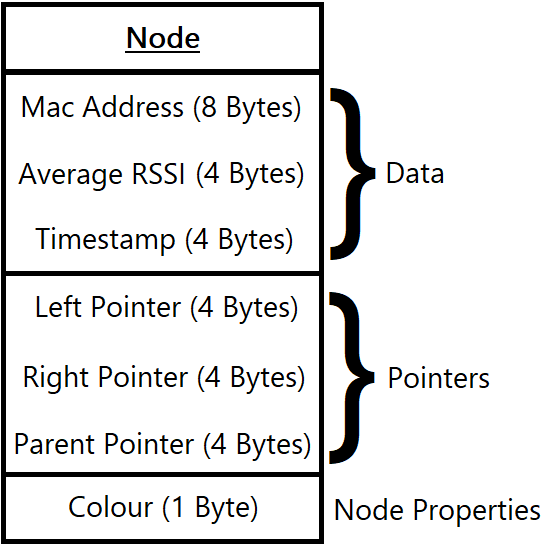
\includegraphics[width=0.4\linewidth]{images/rbtree_node.png}

    \caption{ Structure of a node within the red-black tree. The node is grouped into three sections: the actual data, the pointers to related tree nodes, the colour property of the node (either red or black). }

    % use the notation fig:name to cross reference a figure
    \label{fig:tree_node}
\end{figure}

The implementation of the red-black tree is too long to include here; I will give a brief overview of how this data structure operates. The red-black tree is a self-balancing binary search tree (BST) with extra constraints. \citet{morris_data_1998} provides the conditions that a red-black tree must satisfy:

\begin{itemize}
    \item Every node is either red or black
    \item Every leaf node is black (in my implementation leaf nodes are null pointers, this has the same effect)
    \item If a node is red, then both its children are black (i.e. a red node can't have a red child)
    \item Every path from a node to a descendant leaf node has the same number of black nodes.
\end{itemize}

Following these conditions ensures that the tree is always balanced, which means that the maximum height of the red-black tree at all times is $2\log{d + 1}$, where $d$ is the number of devices encountered, which is what allows its operations to all be $O(\log{d})$. Insertion and deletion operations make use of rotations. Rotations are operations within the tree that are used to preserve in-order traversal ordering, as shown in Figure \ref{fig:tree_rotation}.

\begin{figure}[!htb]
    \centering
    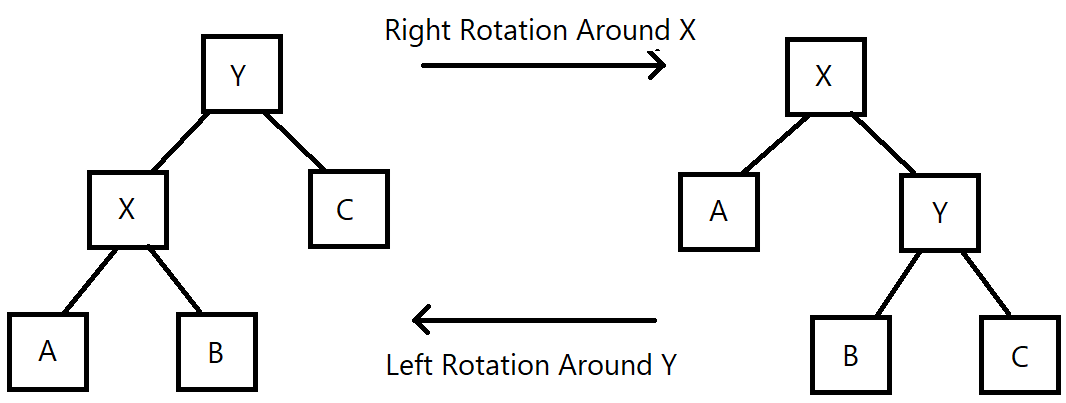
\includegraphics[width=0.8\linewidth]{images/rbtree_rotation.png}

    \caption{ Visualisation of a tree rotation. Re-created version of diagram from \citep{morris_data_1998}. }

    % use the notation fig:name to cross reference a figure
    \label{fig:tree_rotation}
\end{figure}

\section{Android App}

\subsection{User Interface: Pages}

The user interface was designed to be minimalistic so as to not overload the user with information. Power users were a secondary consideration with few options tailored to their use.

For the initial page design, digital wireframing was used. This was done using the Balsamiq \citep{balsamiq_balsamiq_2021} tool. These wireframes were low-fidelity to allow for rapid wireframe prototyping. One reason for using a digital wireframing tool over traditional paper wireframe sketching is that it allows for the wireframes to have a level of mock interactivity to them. This allowed for modelling of the user journey through the UI.

Throughout the initial design, which continued into implementation, the UI was designed to feedback the system state to the user. The system has two states: connected or disconnected. There were two methods of this feedback. First, on every page within the app there is a status indicator icon in the top right of the screen, displaying a checkmark when connected and an exclamation mark when disconnected. Second, some pages change component architecture depending on system state, which allows the user to intuitively grasp the current system state.

For the low-fidelity wireframes the principles of Material Design, \citep{google_design_nodate}, were not followed, this came later during interface implementation. A prime example of Material Design is the bottom navigation bar used throughout the app, Figure \ref{fig:bottom_nav}. Using components and principles from Material Design means that the app will be externally consistent with many existing Android apps. This allows a user to feel a sense of familiarity even during their first use of the app.

\begin{figure}[!htb]
    \centering
    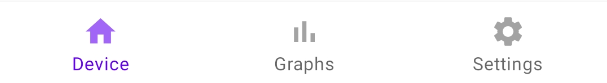
\includegraphics[width=0.7\linewidth]{images/bottom_nav.png}

    \caption{ Example of the bottom navigation bar, a commonly used Material Design component.  }

    % use the notation fig:name to cross reference a figure
    \label{fig:bottom_nav}
\end{figure}

The first page in the user journey is the device connection page. This is presented first, as connecting to the ESP32 is the primary function of the app. It allows two methods of connecting to an ESP32, the user can either scan and connect to a new device or can reconnect to the last connected device. This reconnection option helps in usability for novice users, and more efficient use for advanced users.

This page is then followed by the device information page, assuming the user connects. This information page gives the user an overview of the device they're currently connected to, and contains functionality related to the specific device. This includes: exporting stored data, clearing stored data, renaming the device (remembering mac addresses is difficult), and disconnecting from the device. Both the information page and the home page are accessed via the Device button on the bottom nav bar, Figure \ref{fig:bottom_nav}. The page it goes to depends on the system state, if connected it switches to information, if not connected it switches to the device connection page.

The settings page also responds to system state. When not connected the settings page contains fewer components, Figure \ref{fig:settings_not_connected}. When the device is connected to the app the settings page populates the screen with the connection related components, Figure \ref{fig:settings_connected}. These components are the update device button, and the update status label. These would not be usable when no device is connected so instead of being visible but having an error on use, they are simply hidden.

\begin{figure}[!htb]
    \centering
    \begin{subfigure}[b]{0.47\textwidth}
        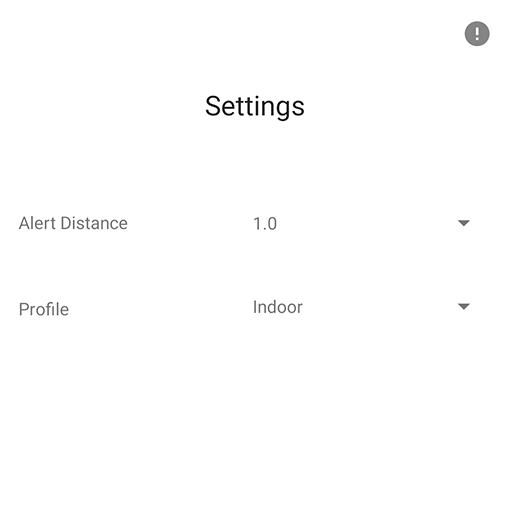
\includegraphics[width=\textwidth]{images/settings_not_connected.png}
        \caption{ Implemented UI for the settings page, when the system state is "not connected". }
        \label{fig:settings_not_connected}
    \end{subfigure}
    ~
    \begin{subfigure}[b]{0.47\textwidth}
        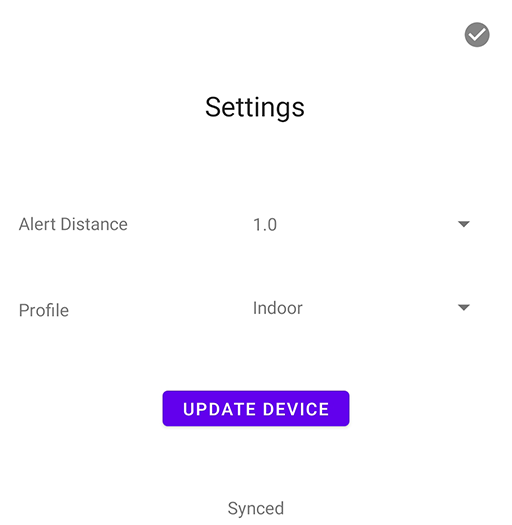
\includegraphics[width=\textwidth]{images/settings_connection.png}
        \caption{ Implemented UI for the settings page, when the system state is "connected". }
        \label{fig:settings_connected}
    \end{subfigure}
    ~
    \caption{ The settings page, as it displays when in both system states. The remaining whitespace on the page and bottom navigation bar have been omitted }
    \label{fig:settings_page}
\end{figure}

From a technical viewpoint the UI was implemented using a base Activity component and a Fragment for each view. The Activity contained elements common between pages such as the navigation bar, and system status icon. Also within this activity was a Fragment container, which allowed for swapping the pages while keeping the same base Activity content. For interacting with the data a View Model was used. This was an abstracted view of the database which all Fragments could access. Android supports this, and by extension supports the Model-View-Controller pattern which was used in this app.

\subsection{User Interface: Visualisation}

Android does not natively support any form of data visualisation functionality. To implement these visualisations an external library, MPAndroidChart \citep{jahoda_mpandroidchart_2020}, was used. MPAndroidChart is a feature rich visualisation library for Android, by default supporting a number of common visualisations such as line charts, pie charts, and bar charts. For each chart supported it comes with a number of animation and aesthetic options; the visualisation renderers can also be extended to implement custom functionality.

For the initial design of the graphs a combination of paper and digital prototypes were used. The weekly interactions bar chart was modelled on Balsamiq along with the rest of the wireframes while the pie charts and interaction trend graph were developed on paper. The interactivity benefit from using digital wireframing was less useful for these so paper prototypes were deemed adequate.

The bar chart represents the interactions per day over the last 7 days, left-most on Figure \ref{fig:app_visualisations}. Its goal is to provide an overview of recent social distancing behaviour, allowing users to check if there has been a spike over a single day. This should allow users to identify problematic behaviour quickly and avoid the cause of the spike. A single colour was used across all bars; having a separate colour per bar would be confusing as it would suggest another layer of data to the visualisation.

\begin{figure}[!htb]
    \centering
    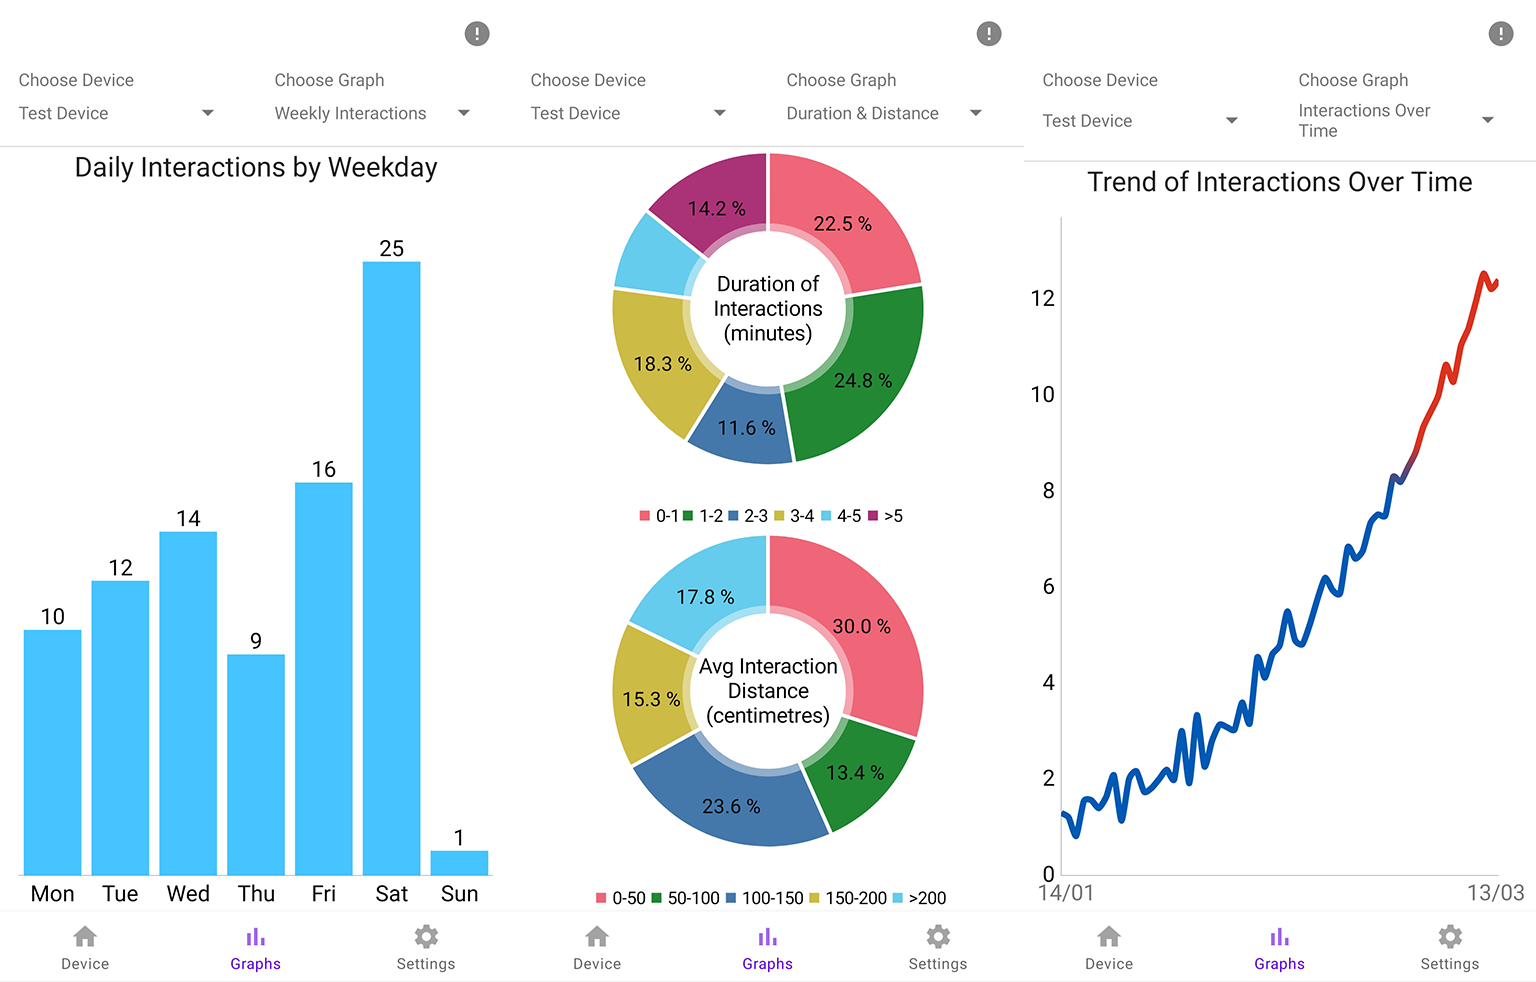
\includegraphics[width=0.78\linewidth]{images/graphs.png}

    \caption{ An example of all three visualisations the app provides. Left shows the interactions per day for the last 7 days. Middle shows time and average distance of all interactions. Right shows the trend of interactions, changing the line colour to red once they are above 8 interactions in a given day. }

    % use the notation fig:name to cross reference a figure
    \label{fig:app_visualisations}
\end{figure}

The pie charts, Figure \ref{fig:app_visualisations}, allow for an aggregated view of the critical factors for COVID-19 infection: duration of contact, and distance of contact. Categories were separated by colour, along with a given key to identify the slices by category. These colours were chosen with particular thought to making the chart as accessible as possible to those with colour blindness. A colour blindess simulator Coblis \citep{colblindor_coblis_2018}, was used to identify problematic colours for each form of colour blindess and check the design. However, there are two forms of colour blindness that this design is not accessible to: Tritanopia and Achromatopsia, simulations of which are shown in Figure \ref{fig:colour_blindess}. Hatching was considered to overcome this, however could not be implemented due to technical constraints of MPAndroidChart.

\begin{figure}[!htb]
    \centering
    \begin{subfigure}[b]{0.3\textwidth}
        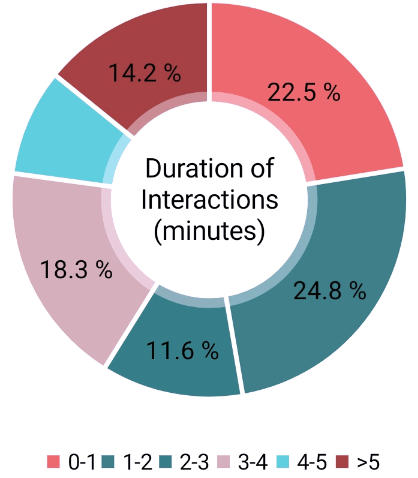
\includegraphics[width=\textwidth]{images/tritanopia.png}
        \caption{ A simulated version of the colour scheme considering tritanopia (blue-blind colour blindess). }
        \label{fig:tritanopia}
    \end{subfigure}
    ~
    \begin{subfigure}[b]{0.3\textwidth}
        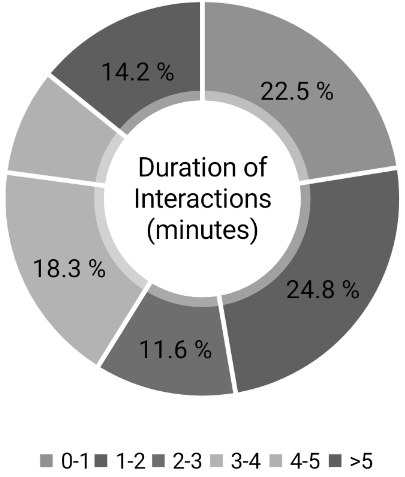
\includegraphics[width=\textwidth]{images/achromatopsia.png}
        \caption{ A simulated version of the colour scheme considering achromatopsia (monochromatic colour blindess). }
        \label{fig:achromatopsia}
    \end{subfigure}
    ~
    \caption{ Simulated version of the two versions of colour blindess this design fails to accomodate. In \subref{fig:tritanopia} it is near impossible to differentiate "1-2cm" and "2-3cm". In \subref{fig:achromatopsia} the shades are not distinct enough to properly differentiate. }
    \label{fig:colour_blindess}
\end{figure}

The interaction trend graph, Figure \ref{fig:app_visualisations}, is designed to be a longer term approach to giving the users the information they need to make decisions about their social distancing behaviour. This forms a trend based on all the interaction data collected from that device, the line changes colour, via a short gradient change, when the interaction trend climbs above 8 interactions. Similar colour blindess considerations and methods were used for the colours here; achromatopsia remains negatively affected by this design. Due to constraints written within the MPAndroidChart library itself having multiple colours along the single line proved challenging. A number of implementation attempts were made. The final implementation achieved this by overriding the shader in the implementation of MPAndroidChart with my own custom LinearGradient shader.

\subsection{Database}

The database is a critical part of the app design and infrastructure, it allows the data collected from the ESP32s to be stored. This allows it to drive the data visualisations discussed above. This makes the Database Management System (DBMS) a crucial component in achieving the key goal of user education.

A relational database architecture was modelled using a Crow's Foot notation Entity Relationship (ER) diagram, Figure \ref{fig:er_diagram}. ER diagrams are especially useful for designing a database schema; ER diagrams typically map very well onto relational databases, more work has to be done for many-to-many relationships however these are not used in this project. To summarise the schema, there are three entities. Device,  which encapsulates the relevant information about the physical ESP32 device. Interaction, which stores all the necessary information about an encounter. RSSI, which is a representation of a single RSSI value logged. An Interaction occurs between two Devices, which is represented as two distinct one-to-many relationships. An Interaction is made up of many RSSI values, which again is represented using one-to-many relationships. In one sentence this can be described as: A device can be part of many interactions, which may contain many RSSI values.

\begin{figure}[!htb]
    \centering
    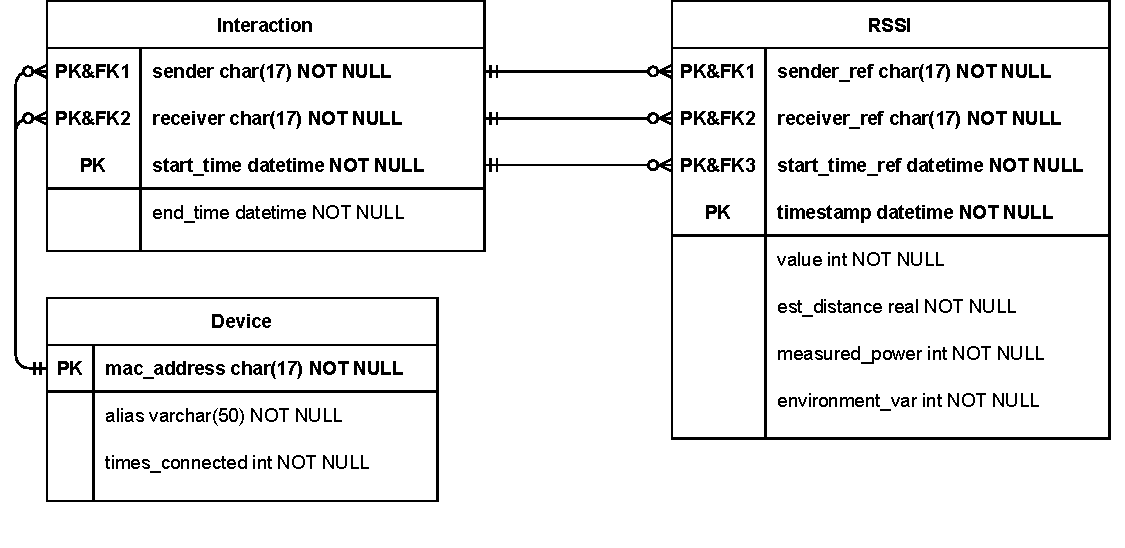
\includegraphics[width=0.9\linewidth]{images/rssi_er.pdf}

    \caption{ A Crow's Foot notation Entity Relationship (ER) diagram used when designing the database structure. Interaction and RSSI contains a compound key. }

    % use the notation fig:name to cross reference a figure
    \label{fig:er_diagram}
\end{figure}

The database was implemented using the Room persistence library, which is part of the Android SDK. Room provides an alternative to working with the raw SQLite database that Android makes use of. It provides a layer of abstraction over the SQLite DBMS while still allowing full control. This is the officially recommended DBMS for Android. It offers a distinct advantage of compile-time SQL query checking, this reduces the chance for runtime errors to occur due to the database. Another problem with using SQLite directly in Android, which Room solves, is that the SQLite application programming interface (API) requires significant repetitive boilerplate code.

Room is split into three primary components: The room database object, the data access objects (DAO), and entity objects. Having the entities modelled as objects allows for query results to be easily captured and used throughout the app. Within each entity Java annotations are used to model attribute properties such as if it's a primary key, or the attributes nullability. Annotations also allow mapping foreign key contraints to defined attributes. The DAO are modelled using interfaces, and their purpose is to provide the database interactions for a given entity. This means there is a one-to-one mapping of entity classes to dao interfaces. They have default annotations for insertion, deletion, and updating. And allow for full custom SQL queries to be run on the underlying SQLite DBMS.

The final layer is the database object itself. It is modelled using an abstract class, which contains static variables and functions. In my implementation I included a ExecutorService references for reading and for writing. The executor services allow queries to be run in a separate thread, asynchronously, preventing the app from visibly pausing when interacting with the DBMS since these operations are not instant. Finally, as part of this class I used a singleton pattern, as recommended by the Room documentation, to ensure that only one instance of the Room database is created during the apps runtime, Figure \ref{cde:singleton}. A singleton pattern just prevents a class from being instantiated more than once.

\begin{figure}[!htb]
    \lstinputlisting[language=java, basicstyle=\small]{snippets/singleton.java}
    \caption{ Singleton pattern implementation for Room instance creation. Also includes threading locks to prevent two executor services from trying creating a database at the same time due to a data race. }
    \label{cde:singleton}
\end{figure}

I also implemented an abstraction layer, called a repository, between the DAOs and the ViewModel. These allowed me to make use of the queries within the DAO, while also wrapping the database calls within the executor services. This was not possible within the DAO as the Java code is generated at compile-time based on the SQL queries. It also allowed me to create more complex operations, such as the case where a device is being inserted but already exists in the database, so is retrieved and has the "times\_connected" attribute incremented, then updates the related device within the database.

One of the technical challenges faced was the incompatibility of the Java Date object format, used to represent and manipulate the date/time information, and the SQL storage of date/time. Forunately, Room provides annotations for specifying custom type convertors. I made the decision to store the date/time information in the database as a long integer, which represents the number of milliseconds in the 1st January 1970, known as Unix Time. This required two type converters, one to convert from a date object to a long integer, and another to covert a long integer to a date object. Doing this also made it possible to select ranges of dates, which was used extensively during visualisation.

For the construction of the average distance pie chart there was a particularly complex SQL query required, Figure \ref{cde:sql}. The aim of this query is to return the number of encounters whose average interaction distance falls within a specified range. For example, the number of encounters that, on average, were 1 metre to 1.5 metres apart. This was achieved by using a parameterised nested SQL query. It had to be parameterised as there were a number of ranges to check, one for each category on the pie chart. It would be bad programming practice to simply copy these queries and hardcode the values in them. A nested query is one which contains multiple queries, in this case two, to allow for intermediate results to be used. Here the inner query is used to obtain the average value of all RSSI values within an interaction for a given receiver device mac address within a given range. This requires using a join between the Interaction and RSSI tables, then getting the average of the RSSI values using the aggregate function AVG. Finally it checks if it falls within the range. Then, the outer query counts the number of values returned, using the aggregate function COUNT.

\begin{figure}[!htb]
    \lstinputlisting[language=sql, basicstyle=\small]{snippets/average_dist.sql}
    \caption{ Parameterised nested SQL query, :receiver is the mac address of the device, :start\_range is the beginning of the distance range, :end\_range is the end of this range. }
    \label{cde:sql}
\end{figure}

The final key function within the data management system is the custom export functionality. This allows the user to export the data stored within the database about the currently connected device, into an external format. This functionality is aimed at power-users who wish to use their data for custom visualisations outwith the app, or to perform custom data analysis. I chose to use the comma separated values (CSV) file format to export the data, as it maps well to the table structure of relational databases. Each table in the database schema is mapped to a separate csv file. The header row of the csv file is constructed using the attribute names within the table. There are many areas where it is possible for this process to fail, so it is designed to fail gracefully. Whenever an error is encountered during exporting, it aborts the process and provides an Android toast, a popup message, to the user detailing the error.

\subsection{Communication}

As previously mentioned, to communicate with the ESP32 device. The Bluetooth libraries included in the Android sdk are low-level and require a lot of boilerplate code and management to communicate at a basic level. During the initial stages of implementation I attempted to use the low level libraries and write a custom high-level BLE management library. This was challenging and was taking too much time from development of key project areas, so the decision was made to refactor my code to make use of the high-level BLE library Blessed \citep{welie_weliemblessed-android_2021}. As this project is under active development with frequent releases I restricted the project to use library version 1.29 to prevent library updates breaking app functionality.

The majority of BLE communication functionality was abstracted from UI Fragments into a custom Bluetooth handler class. This primarily handles the required operations after a change in BLE state. For example, after a disconnection the references held to all the Bluetooth GATT characteristics need to be nullified as they are no longer valid; attempting to use them would crash the app. They also provide an interface for page specific functionality to get and set a select few BLE properties, these properties are not critical to BLE operation so are safe to be changed. The BLE handler also manages the Bluetooth related system permissions which is one of the most critical app functions. If this is not correctly requested then Bluetooth will not function at all. Specifically, it checks if the "ACCESS\_FINE\_LOCATION" permission has been granted. If it has not it requests this app permission from the user. This check needs to happen whenever any BLE operation is executed.

The only BLE functionality not encapsulated by the handler is event based page specific behaviour. For event based functionality that was consistent across all the UI in the app the callbacks were implemented in the base Activity class. This included calling the relevant handler functions when connections or disconnections were occurring, service discovery, and receiving incoming RSSI values. For page specific behaviour, such as hiding and showing components on the settings page, BLE callbacks were defined in the Fragment. To call the page specific call backs an interface was defined IBluetoothImplementer, which specified a contract for implementing two getter functions, one for a BluetoothCentralCallback, and another for a BluetoothPeripheralCallback. The Fragments implement this interface which allows the base Activity to activate the Fragment BLE callbacks from the main BLE callbacks.

\subsection{RSSI Storage + Processing}

This is the parallel to the RSSI transmission discussed in the ESP32 section. The app needs to recieve and decode the RSSI packet to be able to store the RSSI information in the database. This process is started when a characteristic update event is receieved from the Blessed BLE library. As previously mentioned the base Activity callback captures this event.

To understand how the overall RSSI processing system works it is first important to understand the timeout system. This system is required to chunk receieved RSSI values into the relevant interaction. A cut off was set to separate interactions, if more than three seconds had passed between RSSI values then they were counted as separate interactions. This was implemented using a hash map, and a custom TimeoutData class. This allowed mapping mac addresses to these custom objects. These objects stored the start and end time for the interaction, and on updating it would check if the gap was more than 3000 milliseconds. If this was the case, a new interaction had occurred so the start and end time were set to be the new time. Otherwise just the end time would be updated to signify the interaction getting longer.

When a new RSSI value is receieved the system uses byte buffers to easily convert the received bytes to the correct data types. Byte buffers also natively support endian conversions, making this step simpler. Once this data has been decoded it begins the process of inserting this data into the database. First the device is inserted. For interactions, using the timeout system allows for an easy way of updating interactions when presented with new RSSI values. The timeout system is updated with the timestamp of the newest packet, then the start time is retreived from the hash map. This gives the correct start and end times for the current interaction, so the interaction in the database is inserted or updated if it already exists. Finally, now that the interaction has been updated the estimated distance is calculated using Equation \ref{eq:rssi-to-distance}. This provides the final piece of information to insert this new RSSI value into the database.

The base RSSI and bulk RSSI packets are processed in mostly the same way. The bulk RSSI packet has a separate instantiation of the timeout system to prevent interference when both bulk RSSI and base RSSI packets are receieved at the same time. Also the timestamp offset is extracted from the bulk RSSI packet. This is then used to calculate the timestamp by subtracting the offset from the current time. The base RSSI timestamp is just the time it arrives.

\subsection{Device Configuration}

To allow the system to be suitable for a number of environments and scenarios it had to be configurable. Since the device had no means of input from the user this had to be done on the app. This was accomplished by having two configuration options the user could modify, each with pre-set categories. First, the user could change the range they would like the device to be sensitive to other devices. They could also change profile to one of three profiles: Indoor, Outdoor City, and Outdoor Nature. These profiles internally consist of a measured power value, and an environment value. They are coupled into a profile to make the system more usable; it is much more intuitive to say you are indoors rather than saying your measured power is -78 and the environmental factor is 2. This data is packed into bytes, in the format given in Figure \ref{fig:config_packet}, using a byte buffer. This packet is sent to the device to update its settings at two times. First, when the user wants to update the device settings via a button press. Second, when the device first connects. This is necessary as the devices can't store configuration changes between power cycles, due to a lack of non-volatile storage.

\section{Design \& Implementation Summary}

This chapter discussed the high-level design and implementation process used during the project. Key topics and interesting technical areas were discussed in greater detail. Also highlighted, were some of the technical challenges faced throughout the implementation process such as endianess conversion and BLE implementation. The software engineering practices discussed were critical to being able to manage and implement two separate codebases.

%==================================================================================================================================
\chapter{Evaluation}

\section{Testing}

Unit testing was performed for both the ESP32 codebase and the Android App codebase, a total of 129 unit tests were written between the two codebases. The unit tests were created to ensure correctness of implemented code. For each function tested, both normal input and edge case input were tested. Unit tests don't guarantee correct execution but they do help in finding some bugs that exist within the code. On reflection, I should have followed a test-drive development (TDD) approach throughout the project rather than testing at the end, followed by bug fixing. This would have made the constant refactoring during the project far safer, and saved trouble from unseen bugs persisting through iterations during implementation.

\subsection{Android UI Testing}

UI testing was considered and had some attempts to be used in the project using the Espresso UI Test Recorder as part of the Android Studio framework. This allows you to record a set of actions then create assertions on certain UI components to verify their correctness. Unfortunately, this was not suitable for this project as the UI in this project is dependant on BLE interaction with the ESP32 device. Without this interaction it makes certain parts of the UI impossible to test and this framework doesn't allow for mocking this behaviour. Further, since the database operates asynchronously from the UI using the test recording framework isn't reliable since results may vary depending on execution timing. For these reasons the UI of the Android app contains no automated testing.

\subsection{Android Unit Testing}

There are two types of unit testing available on Android. There is Java Virtual Machine (JVM) unit testing and instrumented unit testing. Instrumented unit testing runs either on the phone or within a smartphone emulator; these tests are much slower to execute as they need to upload to the smartphone. JVM unit tests are much quicker but are difficult implement as the Android functionality that an app relies upon can't be executed. To enable implementation of JVM unit testing Robolectric \citep{robolectric_robolectric_2019} was used. This is a library which mocks many common Android SDK function calls. Further, to allow testing components which handled BLE objects Mockito \citep{faber_mockito_2020} was used. Mockito is a library which allows for custom behaviour mocking of certain object types. By using these two libraries, along with the base unit testing library JUnit, \citep{junit_team_junit_2020}, I was able to implement my unit testing within the JVM.

There were some components that were not feasible to test at all. Testing the BLE callbacks was not possible, this is due to how Android, and by extension Blessed, handles callback events. They are declared final, meaning that Mockito is unable to mock a call to them as final classes cannot be extended. This means code contained within the callbacks cannot be covered by tests. Further, the auto-generated code from Android navigation was excluded from testing as this is the domain of UI testing, whereas the auto-generated code from the Room DAO was left in to show the tested state of the database system. A total of 86 unit tests were written for the Android codebase, all of which passed.

Figure \ref{fig:android_coverage} shows the coverage report generated from running the test suite. Unfortunately, the most precise metric this test suite can provide is line coverage, more fine-grained metrics such as branch coverage and condition coverage can provide greater insight. As expected the Activity, Fragment, Visualisation, and DatabaseUI sections of code, which are responsible for UI, are very poorly covered. The main database functionality was aggressively tested, as seen by the 100\% line coverage of entities and repositories. The DAO and main Database package coverage is lower as these packages contain code that is auto-generated, so is harder to design tests for. Overall the line coverage is 44.7\%, including auto-generated and UI sources.

\begin{figure}[!htb]
    \centering
    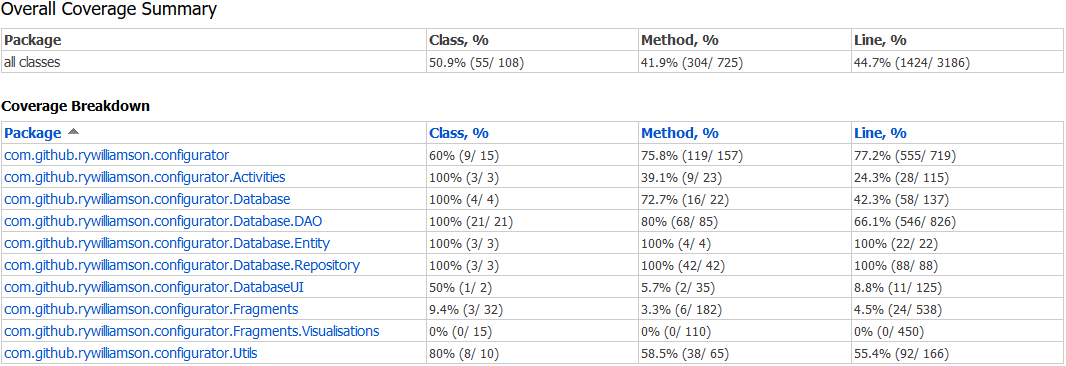
\includegraphics[width=1.0\linewidth]{images/android-code-coverage.png}

    \caption{ Code coverage report generated by IntelliJ IDEA coverage framework. }

    % use the notation fig:name to cross reference a figure
    \label{fig:android_coverage}
\end{figure}

\subsection{ESP32 Unit Testing}

AUnit, \citep{park_bxparksaunit_2021}, is the library chosen to perform unit testing on the ESP32. It is a unit testing framework compatible with Arduino libraries and when compared against similar libraries, such as ArduinoUnit, it runs using less memory. Further, AUnit allows for running the same set of tests on the ESP32 and natively on Linux. For this project I chose to run the tests on the ESP32; the compilation and upload process to the ESP32 is fast and running on the ESP32 allows for avoiding bugs that appear due to architectural differences between ESP32 and Linux. There were no unit testing libraries compatible with Arduino that provided code coverage metrics similar to those in Figure \ref{fig:android_coverage}. As shown in Figure \ref{fig:esp32_tests_pass}, all 45 tests written for the ESP32 passed. These tests targeted: The red-black tree implementation, the circular queue implementation, the configuration endianess conversion, packet creation functions, and other smaller functionality spread throughout the system.

\begin{figure}[!htb]
    \centering
    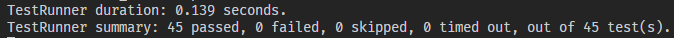
\includegraphics[width=1.0\linewidth]{images/esp32-test-pass.png}

    \caption{ Test report generated by AUnit, showing that all 45 ESP32 tests pass. }

    % use the notation fig:name to cross reference a figure
    \label{fig:esp32_tests_pass}
\end{figure}

\section{Ethics}

A requirement of this system was that evaluation was performed ethically. The survey performed was ethically sound, shown by following and signing the ethics checklist as seen in Figures \ref{fig:ethics_checklist1} - \ref{fig:ethics_checklist3}. The experiment required a request for formal ethical approval, which was granted as seen in Figures \ref{fig:full_ethics_approval1} - \ref{fig:full_ethics_approval3}. These required formal ethical approval as my project used non-standard hardware, namely the ESP32, which violated point 2 of the ethics checklist. As part of the experiment process, participants were asked to fill in a consent form, Figure \ref{fig:participant_consent}, along with receiving information sheets, Figure \ref{fig:participant_information},  and a debriefing email, Figure \ref{fig:participant_debriefing}. Finally, during the surveys performed their was an informed consent section in the Google Form, which the user had to agree to, to begin the survey.

\section{Experiment}

\subsection{Limitations}

Due to the Scottish COVID-19 restrictions of not being able to meet with others that persisted for the duration of this project I was only able to perform this experiment a single time, with those that I lived with. This gives a very small sample size to draw conclusions from. In the results section I will discuss some hypotheses that can be made based on the data collected from the experiment, however these hypotheses may have been shown to be inaccurate if this experiment had been able to run with a larger sample size.

\subsection{Experimental Procedure}

A single experiment was run during this project. The experiment had two aims: to find a real world view of the system's performance, and to understand the usability of the created system. The first aim was achieved through the tasks the participants performed. The second aim was achieved through observation of participants, and feedback they provided. The experiment consisted of two participants. The tasks the participants had to perform can be broken into two categories: device based tasks, and app based tasks. The experimental procedure is outlined below.

First, have the participants choose three arbitrary locations within their home or within their garden, if this experiment were to be performed with many groups the wide number of environments would provide more reliable data. Then, each participant is separately asked to turn the devices on and connect the device to the app. The participants should not see each other during this stage as they may learn from each other which would compromise the evaluation of system usability, however if the participant struggled to do this then I should help and note this down.

Once both participants have completed setup, have them stand 3 metres apart, using a tape measure of 3 metres length between them as seen in Figure \ref{fig:experiment_setup}. The devices should not be interacting at this stage; 3 metres should be a larger distance than the maximum size profile. Now, the participants are asked to ensure the devices are set to the relevant profile and a distance of 2 metres, with this being checked to be correct. One participant should now be instructed to move towards the other, stopping when the devices alert the user and having the observer record the distance apart. Then they are asked to move backwards until they stop interacting, again recording this distance. Now the other participant should perform these tasks. This is repeated for 1.5 metre, and for 1 metre configurations, then again for each of the other two locations.

The participants are then separated again. They are each asked to explore the app further, speaking their thoughts during the process. These are written down as a think-aloud evaluation, which allows collection of qualitative data on the app usability. Finally, the participants are asked to disconnect the devices, turn off the devices, and complete a Google Forms survey, Figures \ref{fig:survey-questions-1} - \ref{fig:survey-questions-2}, about their experiences with the app.

\begin{figure}[!htb]
    \centering
    \includegraphics[width=0.95\linewidth]{images/experiment.png}

    \caption{ Example of how the experiment would be setup in a given area. Participants stand at each end of the tape measure which is 3 metres in length. }

    % use the notation fig:name to cross reference a figure
    \label{fig:experiment_setup}
\end{figure}

\subsection{Device Tasks}

These tasks involved the participants interacting with the physical ESP32 microcontroller, and using it to attempt to stay socially distant from the other participant. These tasks were created to ensure the participant interacted with the board, and allowed an insight into the intuitiveness of the physical device with little to no instruction. The specific tasks were turning on the device, using the devices to social distance, trying both alert types, and turning off the device. The device data was collected at the end of the experiment to cross reference what distance the device believed the participants were from each versus the real physical distance.

\subsection{App Tasks}

These tasks involved the particpants interacting with the Android app. This, along with the questionnaire, provides the information on usability. During these tasks the participants explore the data visualisations within the app. Part of the evaluation is observing how clear these visualisations are to the participants, and also aiming to understand how well these visualisations educate the user on their current social distancing. Since doing this with the data collected from the experiment alone would not capture the full breadth of the visualisations, a fake device was inserted into the device list that they are instructed to choose. This could be problematic in that the data in the visualisations doesn't personally relate to the participants, so they may have reacted differently to real data. However, this could only be overcome by running an experiment in an environment where multiple people would be using the devices daily, which was not feasible for this project.

\section{Qualitative Survey}

To attempt to account for the COVID-19 limitations described above a separate survey was created that could be sent to participants online, Figures \ref{fig:non-contact-survey-questions-1} - \ref{fig:non-contact-survey-questions-2}. This survey was designed to only look at usability and education. The survey contained a section for each page in the app, a section for the device, and a general questions section. Within each section was a short video, of either the app being operated, or the device being used. These videos were the basis for the questions are were an attempt at a substitute for using the device. This survey received 24 responses, a significant amount, and was segmented into 17 (70.8\%) tech-literate responses, and 7 (29.2\%) tech-iliterate responses. This survey was designed to enable quantitative and qualitative responses; Likert scale, and yes/no questions were used to obtain quantitative data.

\section{Results Analysis}

Different methods were required for analysing quantitative vs qualitative. Open, axial, and selective coding \citep{williams_artofcoding_2019} was used to analyse the qualitative data. There were two sets of quantitative data to analyse: the experiment device and measured data, and the quantitative questions in the surveys.

\subsection{Open, Axial, Selective Coding}

To analyse the qualitative questions in the surveys open, axial, and selective coding was used, with a modification to look at cumulative category mentions. This technique is applied by first reviewing all the qualitative data collected. When reviewing this data open codes are created, which reflect ideas that occur. For example, in my evaluation of the non-contact survey open code 1 was "Correct definition of interaction". Then axial codes are created by reviewing the open codes and looking for commonalities between them, axial codes can also be thought of as categories of open codes. For example, in my evaluation axial code 5 is "Understanding of concepts", which contains open code 1. To derive selective codes a similar process takes place, the links between axial codes are identified and categories (selective codes) are created. Figure \ref{fig:oas_codes} shows a partial open, axial, selective coding workbook. In additonal to produces these codes I derived a cumulative total of mentions for each axial and selective code by each participant. This is used to obtain a participants overall feelings on the system, and when totalled across participants it provides a view of how the system performed with regards to usability overall.

Finally, for this project I performed two separate sections of open, axial, and selective coding. One for the post-experiment survey and another for the non-contact survey. This was to allow for separate analysis, as participants who have used the device had a different experience with the system. Henceforth, codes from the experiment will be prefixed with 'E', and codes from the non-contact survey will be prefixed with 'N'.

\begin{figure}[!htb]
    \centering
    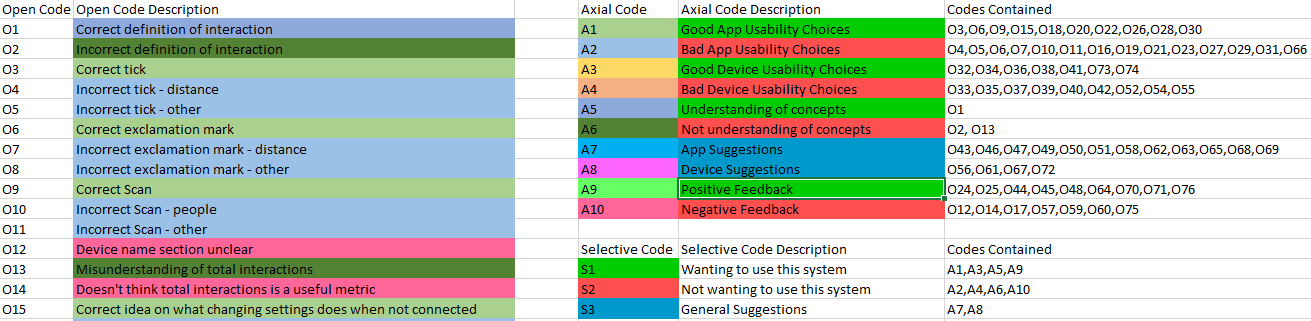
\includegraphics[width=1.0\linewidth]{images/codes.png}

    \caption{ Excel workbook of the open, axial, selective code process. Contains a small subset of open codes, all axial codes, and all selective codes for the non-contact survey evaluation. }

    % use the notation fig:name to cross reference a figure
    \label{fig:oas_codes}
\end{figure}

\subsection{Quantitative Analysis: Survey Data}

For both the post-experiment survey and the non-contact survey Google Forms were used in the collection of data. Part of this data is quantitative, using Google forms Likert Scale, and multiple choice question types. Part of the Google Forms functionality is to create categorical data visualisations based on the received question responses. Having these visualisations allowed for easier analysis by inspection.

\subsection{Quantitative Analysis: Experimental Data}

Two dependant variables were considered during the experiment: the physical distance when alerts started and stopped, and the device data throughout the experiment, which was extracted using the export data feature of the system. After the experiment had concluded to device data was processed to extract the timestamps of each interaction. These timestamps were then analysed to map the real distance measurements to the device recorded data, i.e. map the device belief to the observed distance. Once the timestamps for the start and end of each user task had been located they were extracted and estimated distances were calculated from the related RSSI data.

This data was used to calculate important key metrics, such as: difference in reaction time between the two devices, and the difference between the real distance between participants and the distance set in the profile. These metrics were then used to create data visualisations to provide insight, for or against, some hypotheses which will be disucssed in the Findings section. Due to only being able to carry out a single experiment due to COVID-19 limitations described above, the data here can neither prove nor disprove any claims as there is not enough data to perform statistical tests with sufficient confidence levels.

On reflection, a better approach to the experiment would have been to record the participants performing the walking task from a top-down perspective. This would have provided an easier, and possibly more accurate, method of mapping the device belief to real data. Further, this would have allowed further exploration and analysis of the data as the speed could be calculated and taken into account.

\section{Findings}

I will break down the findings using the open, axial, and selective codes defined above to highlight significant and unexpected results from the analysis. Each section will contain analysis from both qualitative and quantitative data to illustrate these key findings.

\subsection{In Favour of System Use}

In total, during the non-contact survey, participants commented on more positive attributes than negative with 256 codes in favour of the system compared (NS1) to 168 attributes against system use (NS2). This section will discuss a few key aspects that were expressed by participants as particularly good.

First, the data visualisations on the app were particularly well received, especially in regards to prompting behavioural change in users, Figure \ref{fig:behaviour}, which suggests the users were learning useful information from these visualisations helping achieve the system goal of education. The large impact of the trend interaction graph was further explored and can be backed up with qualitative feedback. The trend graphs were well understood with all but one participant understading the x-axis, 20 understanding the y, and 18 understanding the gradient colour change. The gradient colour change seemed to make a significant impact as it used standard colours for danger (red) and safety (blue), with 15 of the 18 participants who indicated it would change behaviour, also had an intuitive understanding of the colour change meaning. Only a single participant indicated a behviour change for trend without understanding the colour change.

\begin{figure}[!htb]
    \centering
    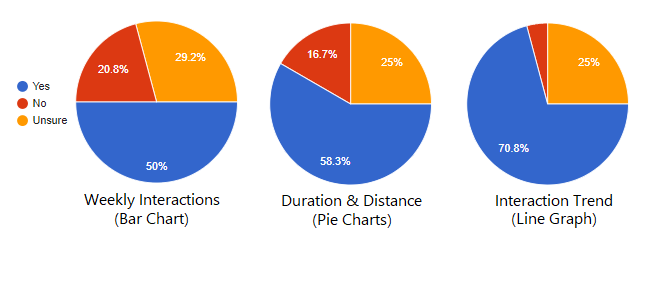
\includegraphics[width=0.9\linewidth]{images/behaviour-graphs.png}

    \caption{ Showing the likelihood that each graph will change participants behaviour. Left is the weekly interactions chart with 50\% of users saying it would change behaviour, middle are the pie charts with 58.3\%, and right is the interaction trend graph with 70.8\% }

    % use the notation fig:name to cross reference a figure
    \label{fig:behaviour}
\end{figure}

The visual method of alerting the user was well understood when given in context. Alerting was evaluated both in context and without context, this was done to discover how a first time user would intuitively understand the system both before their first interaction, and after their first interaction. This resulted in a stark difference with only 6 participants having a correct understanding of the visual interaction alert initially, but once provided with the context of another device moving towards and away 23 of the 24 participants understood. Overall this is positive, with some room for improvement on providing the user with context.

Finally, in terms of general app design, users intuitively understood many aspects of the UI which showed positive usability. Particularly the usage of the clear and export buttons on the device info page were well understood Figure \ref{fig:button_likert}. These results show two components of the overall app that contribute to having 157 total positive app usability codes (NA1) across all participants.

\begin{figure}[!htb]
    \centering
    \begin{subfigure}[b]{0.48\textwidth}
        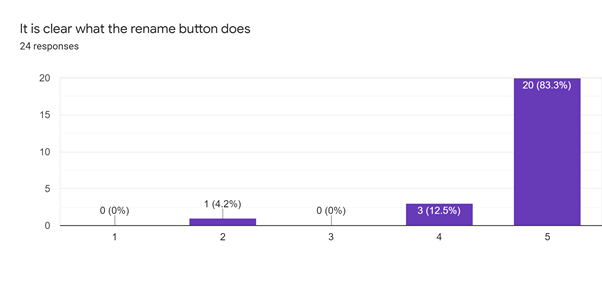
\includegraphics[width=\textwidth]{images/rename_likert.png}
        \caption{ Likert scale for rename button usability. }
        \label{fig:rename_likert}
    \end{subfigure}
    ~
    \begin{subfigure}[b]{0.48\textwidth}
        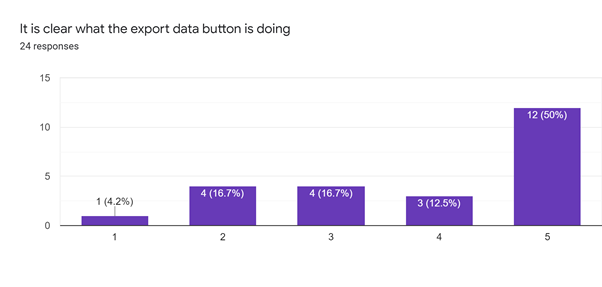
\includegraphics[width=\textwidth]{images/export_likert.png}
        \caption{ Likert scale for export button usability. }
        \label{fig:export_likert}
    \end{subfigure}
    ~
    \caption{ Likert scales for quantitative data collected from the non-contact survey. \subref{fig:rename_likert} shows the feedback on the rename button with 95.8\% of participants having a good understanding, \subref{fig:export_likert} shows the feedback on the export button with 62.5\% of participants having a good understanding }
    \label{fig:button_likert}
\end{figure}

\subsection{Against System Use}

A significant problem with the current implementation of the system is the performance of the physical devices in social distancing. From the experiment, significant difference was found between the real distance participants kept from each other and the distance that should have been kept. In the living room a mean error of 0.32m and standard deviation (std) of 0.18m was found, for the garden a mean of 0.63m and std of 0.48m, and for the hallway a mean of 0.58m and std of 0.6m. This highlights the problems with using Bluetooth RSSI values to estimate proximity, and shows that the categories set by the profile can't be appropriately differentiated between. To back this up, the difference in time between devices alerting can be used as another indicator of this issue. As seen in Figure \ref{fig:clustered-time-diff}, there is often a significant time difference which may cause confusion between system users. This point is backed up in the qualitative analysis through both experiment participants using codes E01, and E02, which are both related to the device not keeping sufficient distance between them.

\begin{figure}[!htb]
    \centering
    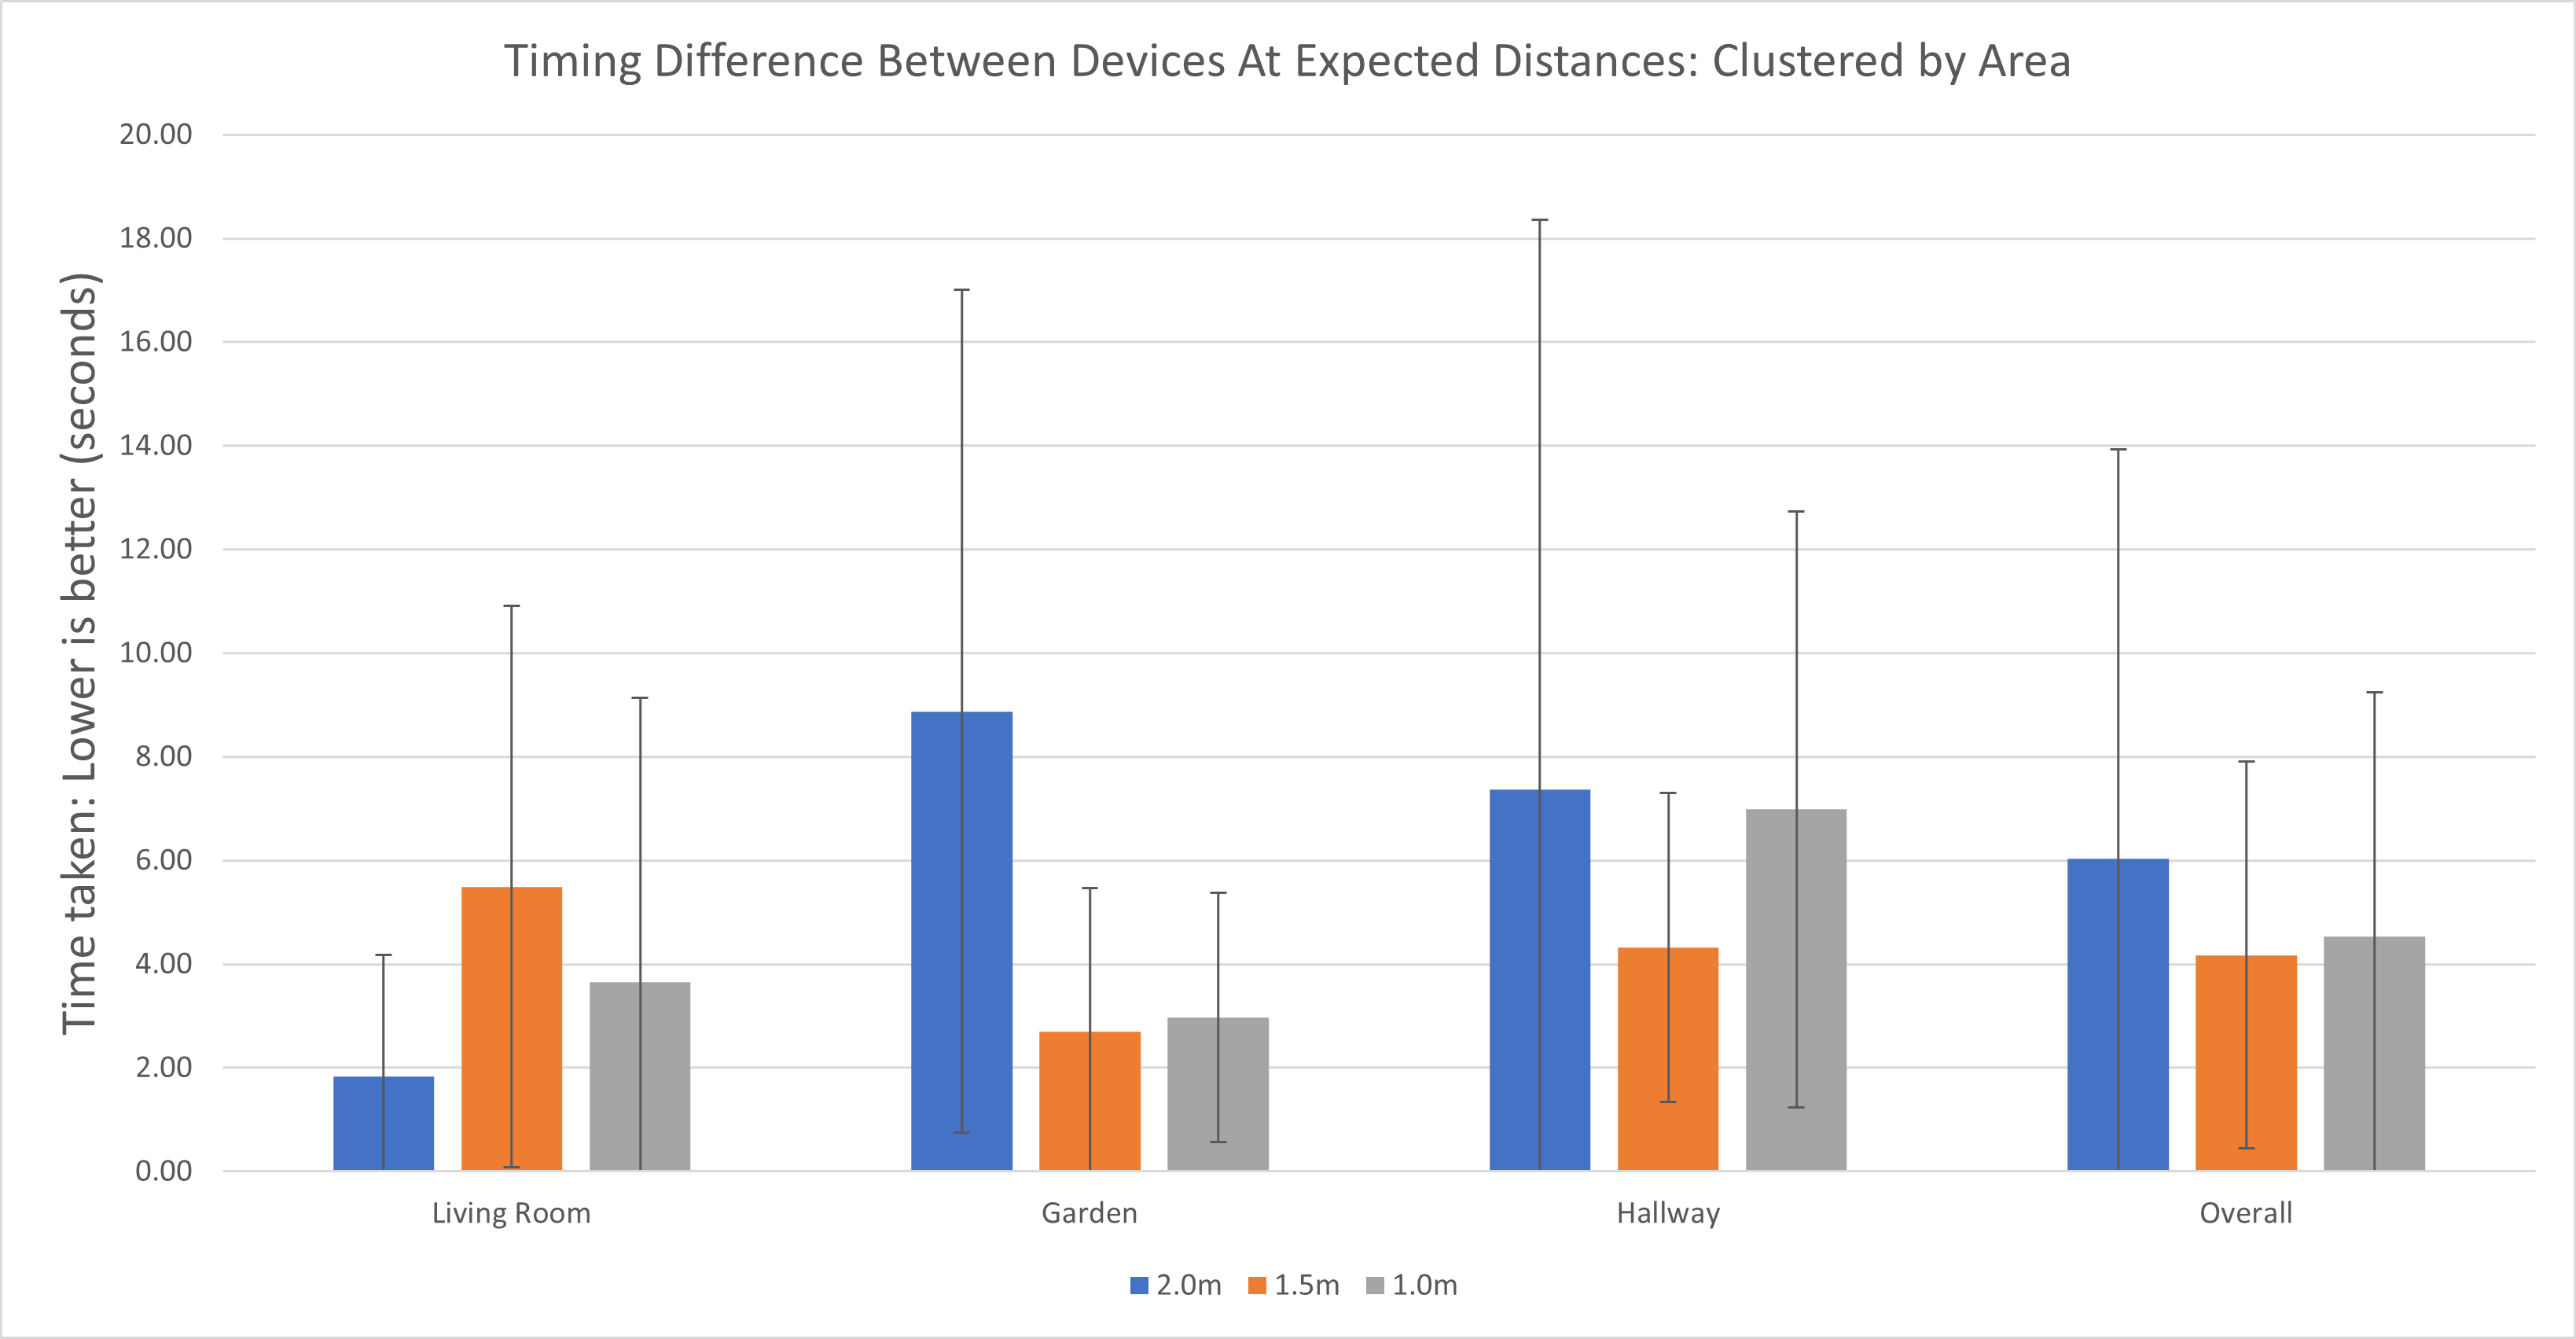
\includegraphics[width=1.0\linewidth]{images/clustered-time-diff.png}

    \caption{ Analysis of mean absolute time differences of devices reacting to change in real world state. Clustered by location, showing the time difference for each distance profile. Error bars are calculated from standard sample deviation. }

    % use the notation fig:name to cross reference a figure
    \label{fig:clustered-time-diff}
\end{figure}

Another aspect that showed a user preference against using this device is poor device usability. Overall there were slightly more negative device usability axial codes (NA04), with 61 code uses, compared to positive device usability axial codes (NA03), with 59 code uses. This is near a "break-even" in usability, however this is a poor result in terms of usability, as this suggests that the current design is unusable by many users. On further examination of the open codes it was found that the open codes related to user misunderstanding of the device log size number accounted for 44 of 61 (72.13\%) negative device usability codes. This suggests that primary device usability issue is how the device log size is presented to the user. This is tricky to solve, as adding in a descriptor of the number, such as "Size: " takes up screen space. At the font size used only 8 characters can fit on a line, with the smaller font size allowing 16 characters. If a smaller font size were used then understanding may be gained, but usability may be lost in terms of users being able to read the text.

\subsection{General Suggestions}

There were many suggestions made during user feedback. Here I will highlight a couple I consider important, or that occurred over multiple responses. First, from the experiment participants, both experienced frustration from the size of the drop-down lists (spinners), they wanted these to be increased; this would improve usability for all users. A common point was participants suggesting a tutorial, or help information, Code NO43. My original goal was to design so this would not be required, however on reflection this was a naïve design decision.

\section{Requirements Validation}

In terms of requirements, as described in Sections \ref{sec:func_requirements} \& \ref{sec:non_func_requirements}, which were not met, none of the "Could Have" requirements were implemented due to time contraints. I would consider the Ease of Use requirement partially met, however there is clear room for improvement. Finally, the precision in RSSI proximity sensing requirement is not met, and would require hardware changes to solve. This means that 6 of 7 must have requirements were met, 2 of 3 should have requirements were met, and 0 of 5 could have requirements were met.

\section{Evaluation Summary}

When considering the evaluation process as a whole it was clear that there was more positive feedback than negative, showing this device has potential for future application. However, there are significant technical and usability issues that would need to be solved before this device could be reliably used to re-enforce social distancing practices. Particularly the current combination of BLE hardware and software support on the ESP32, I will discuss solutions to this primary problem in the future work section.

%==================================================================================================================================
\chapter{Conclusion}

\section{Summary}

This project aimed at building Keep Your Distance, an integrated microcontroller and smartphone system to allow people to be more confident that they were adhering to social distancing practices. ESP32 was the chosen microcontroller, delivering both a low-power and low-cost solution. This introduced some technical constraints which influenced the project. Some constraints were manageable, such as not having any non-volatile storage on-board. Some constraints could not be mitigated against and would require hardware changes, such as the transmission power of the Bluetooth system. In addition to enforcing social distancing there was a focus on user education, allowing users to make changes to their habits based on recorded system use. There was also a focus on system usability, ensuring this system could be used by a wide range of users; considerations were made for aspects like technical knowledge, and colour blindness.

Through user evaluation and testing it was shown that, for both functional and non-functional requirements, all the must have requirements in the MoSCoW framework were met, with a further 66\% of should have requirements being met. The user experiment showed that further development is needed to achieve active contact identification in a precise and timely manner. This is shown by the best of the result sets having a mean error of 0.32m and std of 0.18m, along with a significant time difference in device activation of at minimum 2000 milliseconds. However, both the education and usability goals were met, as shown by the open, axial, selective coding process and the quantitative questionnaire data. For education, all the data visualisation were well understood with the best being the trend graph at 70.8\% of participants reacting positively. In terms of usability, this was shows by the 157 positive app usability codes. This shows the participants had an intuitive understanding of the interface

\section{Future Work}

There have been numerous areas of the project which I have idenitfied areas to focus improvements on if I had more time on the project, or if someone were to continue this project further.

\subsection{Hardware Changes}

There are a number of issues to be solved and improvements to be made, the majority of which can be resolved through hardware changes. The main issue is BLEs poor suitability for real-time accurate distance approximation. The RSSI values are subject to significant variance caused by environmental factors such as surrounding surfaces, surface material, interference from other signals, and people themselves. Additional hardware could be incorporated into the system in the form of Ultra-Wideband (UWB) transmitters. This would allow far more accurate, and precise distance estimation using the Two Way Ranging technique \citep{inpixon_ultra_wideband_2021}.

\subsection{Alternative Distance Approximation Models}

A parallel area for future work would be changing the distance approximation model that is used. Currently the model only takes into account the fluctating RSSI values. More complex models could be created that include temporal aspects as show by \citet{chandel_proxitrak_2020} in the "ProxiTrak" system. These models could be constructed from large datasets using machine learning then deployed onto the ESP32 for efficient use. This has the potential to improve the the accuracy of the distance approximation, but it is unclear if this would solve the timing issues.

\subsection{Multi-platform App}

Currently the companion app is only implemented on Android OS, specifically higher than version 23 of the Android SDK. However, this prevents people who don't own an Android device from being able to use a system, so the app should be implemented to work on other mobile operating systems such as iOS. There is also the potential here for the app to be transferred to operating systems which run on wearable devices.

\subsection{Further Acessibility \& Usability}

While consideration were made for accessibility during this process, such as designing colour sets to work over a wide variety of colour blindness types. However, further work is needed in accessibility for low-vision and blind users. Currently key areas of the app, such as the data visualisations, have no support for screen readers. This should be changed so that no users are excluded from using the system. To improve overall usability help sections should be added to the app, both for information on certain app functionality and to describe the device output to users.

\section{Key Reflections}

Working through the process to create the Keep Your Distance system, allowed the development of many new skills and the consolidation of existing skills developed throughout 4 years of university study. Particularly, I have now seen firsthand the importance of project and time management, along with skills and tools to improve these processes. Working on two distinct but related codebases simultaneously, and interlinking these through BLE networking, has emphasised the value of protocol and system architecture. This project has also allowed me to appreciate the difficulties in anticipating problems during early requirements gathering and analysis, and the further difficulties in mitigating these issues as they arise.

The development process followed iterative design and agile practices, which were beneficial in allowing concepts to be trialed early. However, a great deal of time was spent on locating and fixing obscure bugs that arose from the numerous refactorings applied to the codesbases over the project. If I'd followed a test-driven development approach, there would have been less time spent in solving these issues allowing for more time in feature development.

%==================================================================================================================================
%
% 
%==================================================================================================================================
%  APPENDICES  

\begin{appendices}

    \chapter{Ethics}

    \begin{figure}[!htb]
        \centering
        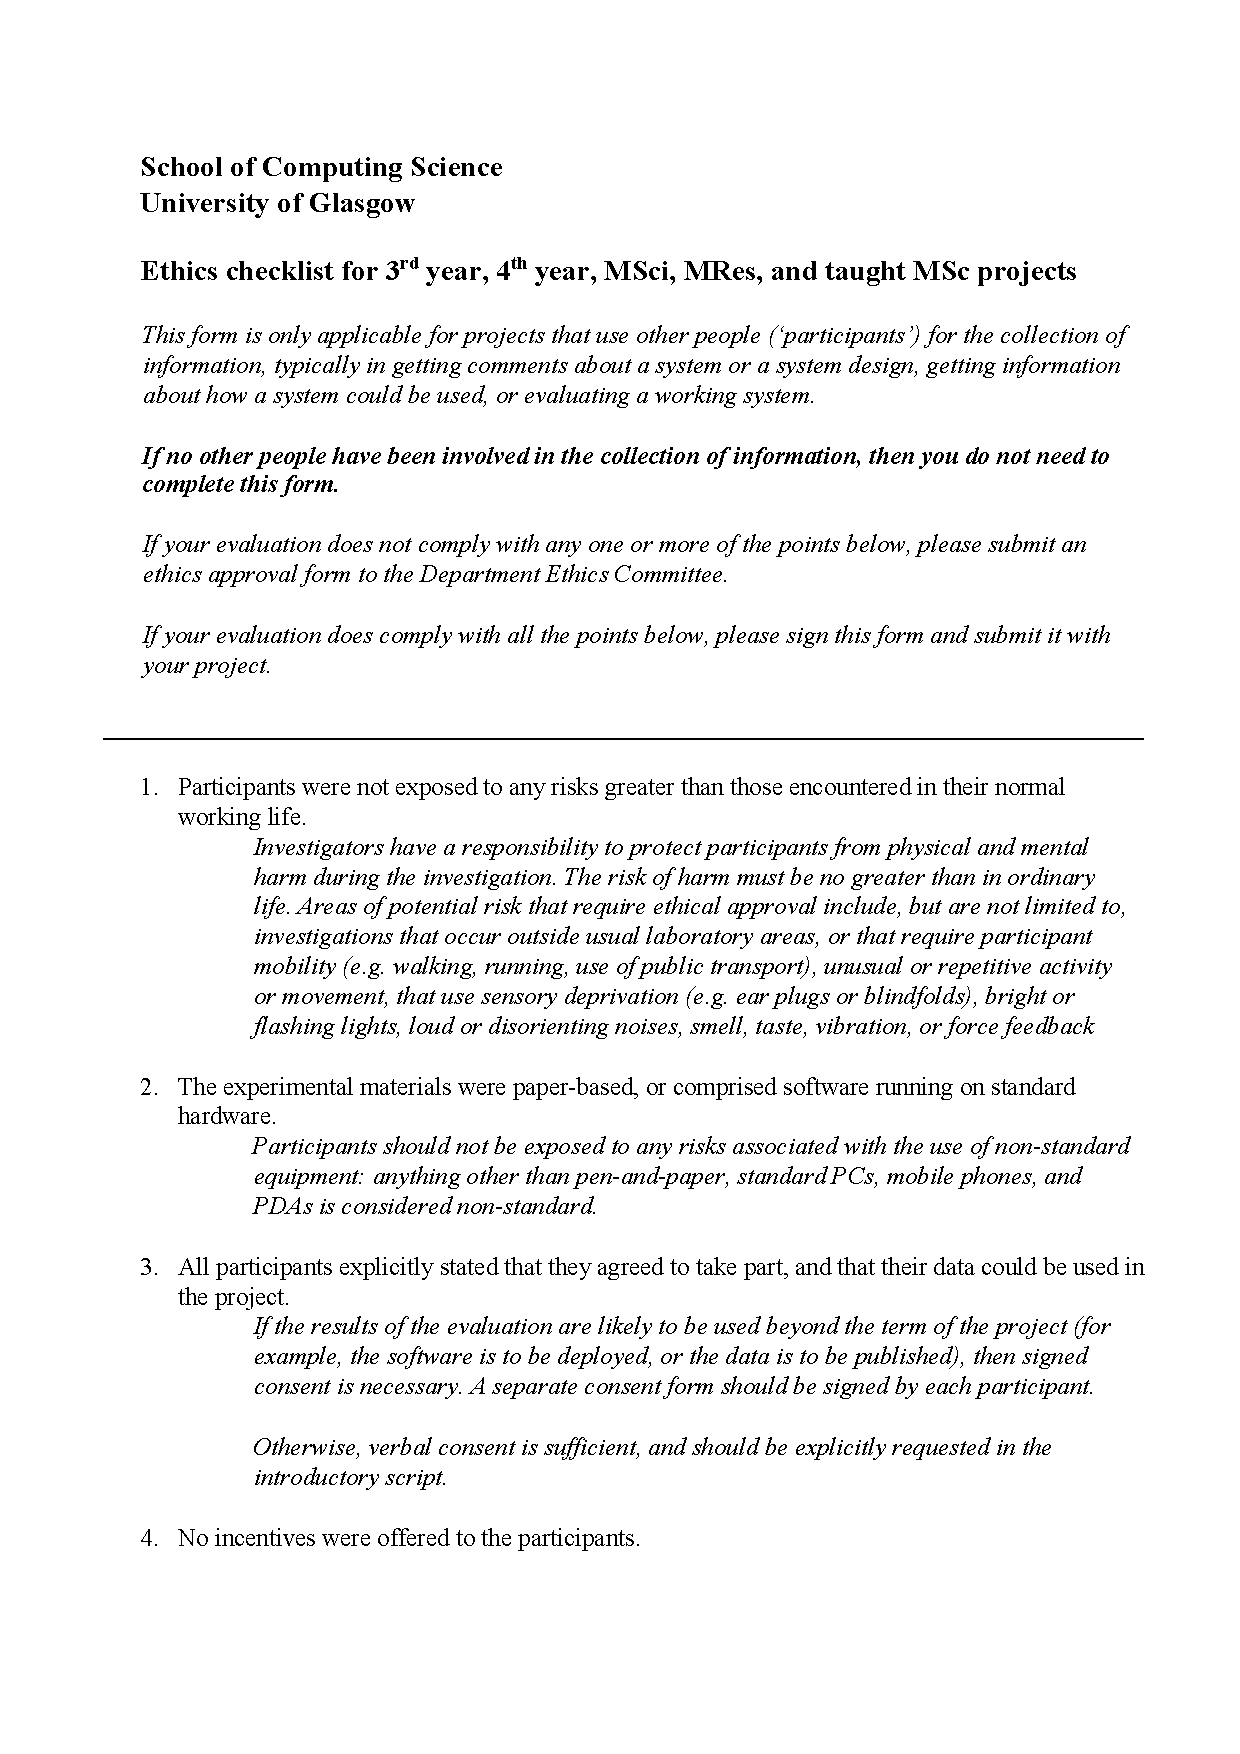
\includegraphics[width=0.8\linewidth]{images/ethics_checklist_signed 1.pdf}

        \caption{ The signed ethics checklist - used for the non-contact survey. Part 1 of 3 }

        % use the notation fig:name to cross reference a figure
        \label{fig:ethics_checklist1}
    \end{figure}

    \begin{figure}[!htb]
        \centering
        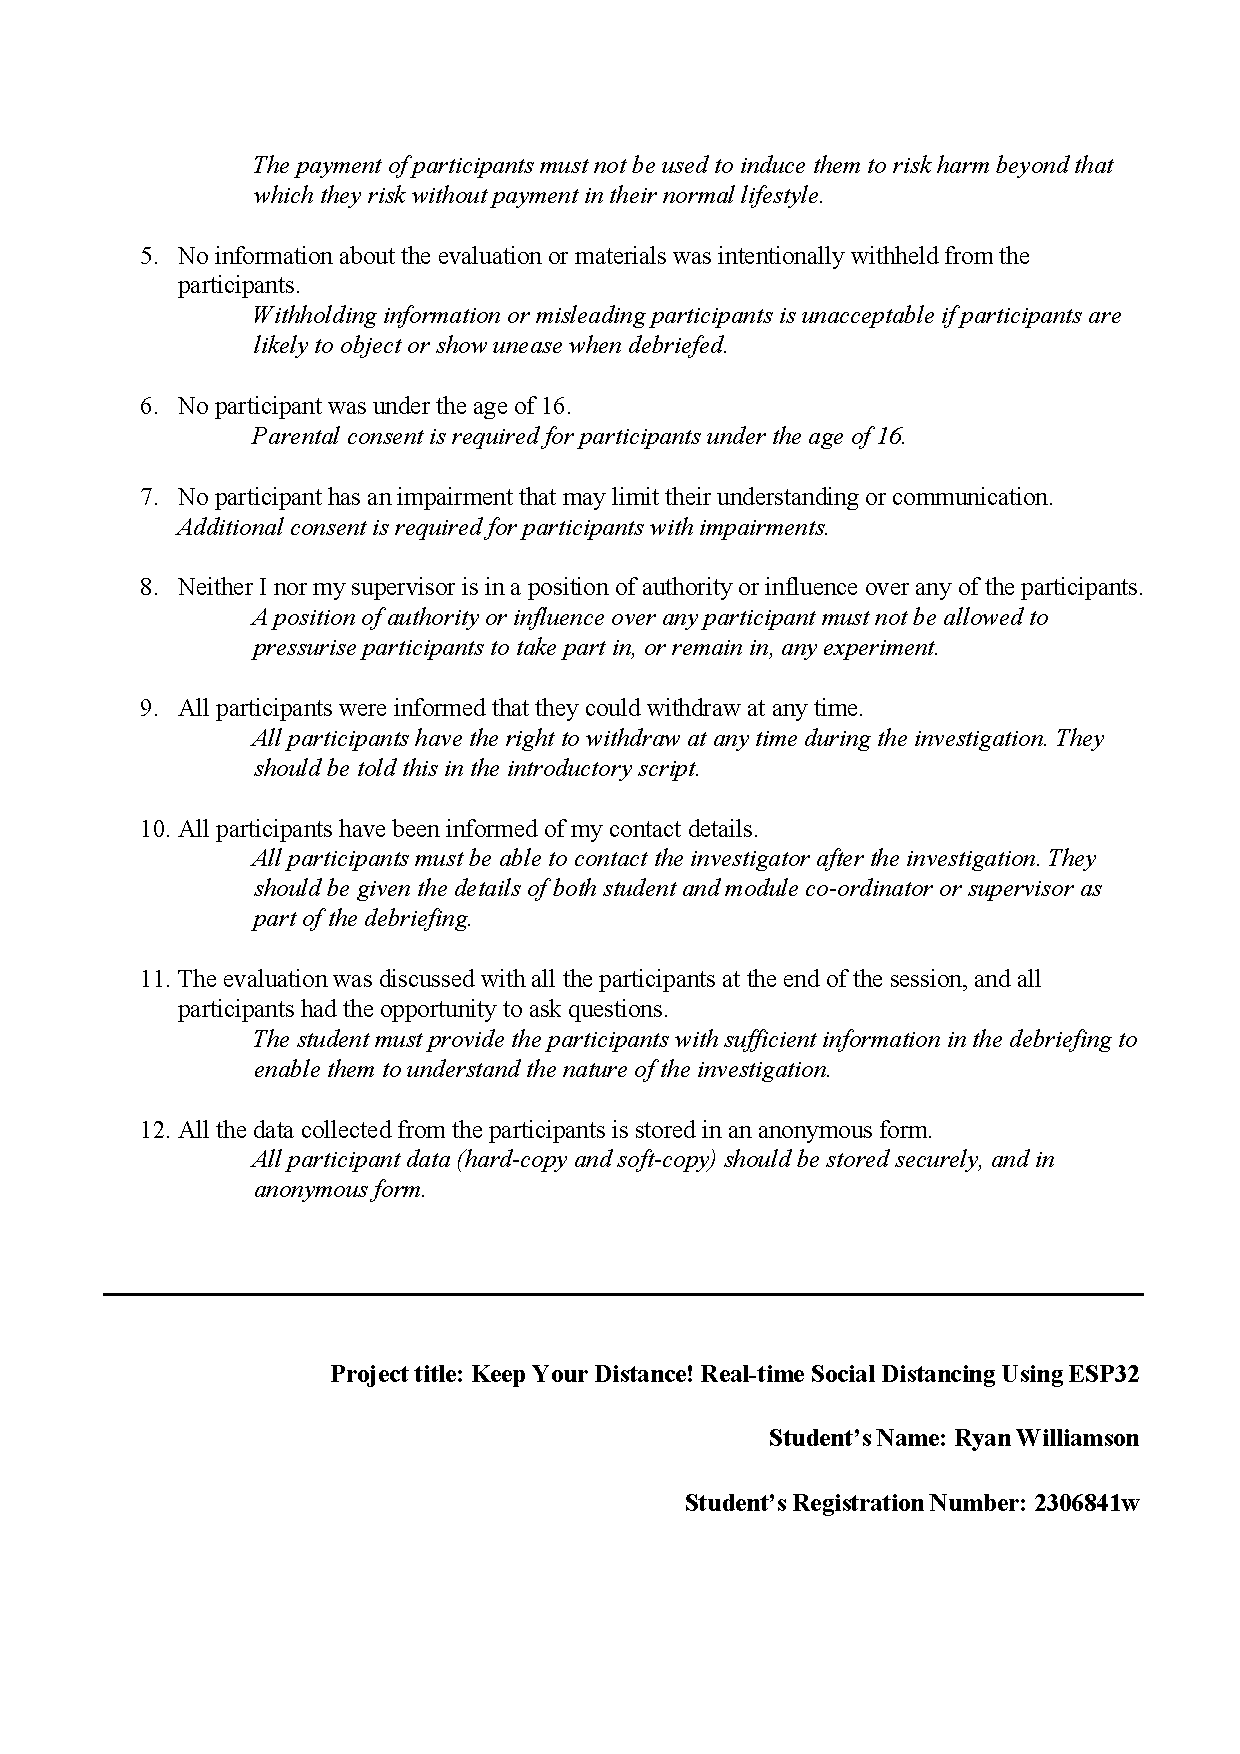
\includegraphics[width=1.0\linewidth]{images/ethics_checklist_signed 2.pdf}

        \caption{ The signed ethics checklist - used for the non-contact survey. Part 2 of 3 }

        % use the notation fig:name to cross reference a figure
        \label{fig:ethics_checklist2}
    \end{figure}

    \begin{figure}[!htb]
        \centering
        
\includegraphics[width=1.0\linewidth]{images/ethics_checklist_signed 3.pdf}

        \caption{ The signed ethics checklist - used for the non-contact survey. Part 3 of 3 }

        % use the notation fig:name to cross reference a figure
        \label{fig:ethics_checklist3}
    \end{figure}

    \begin{figure}[!htb]
        \centering
        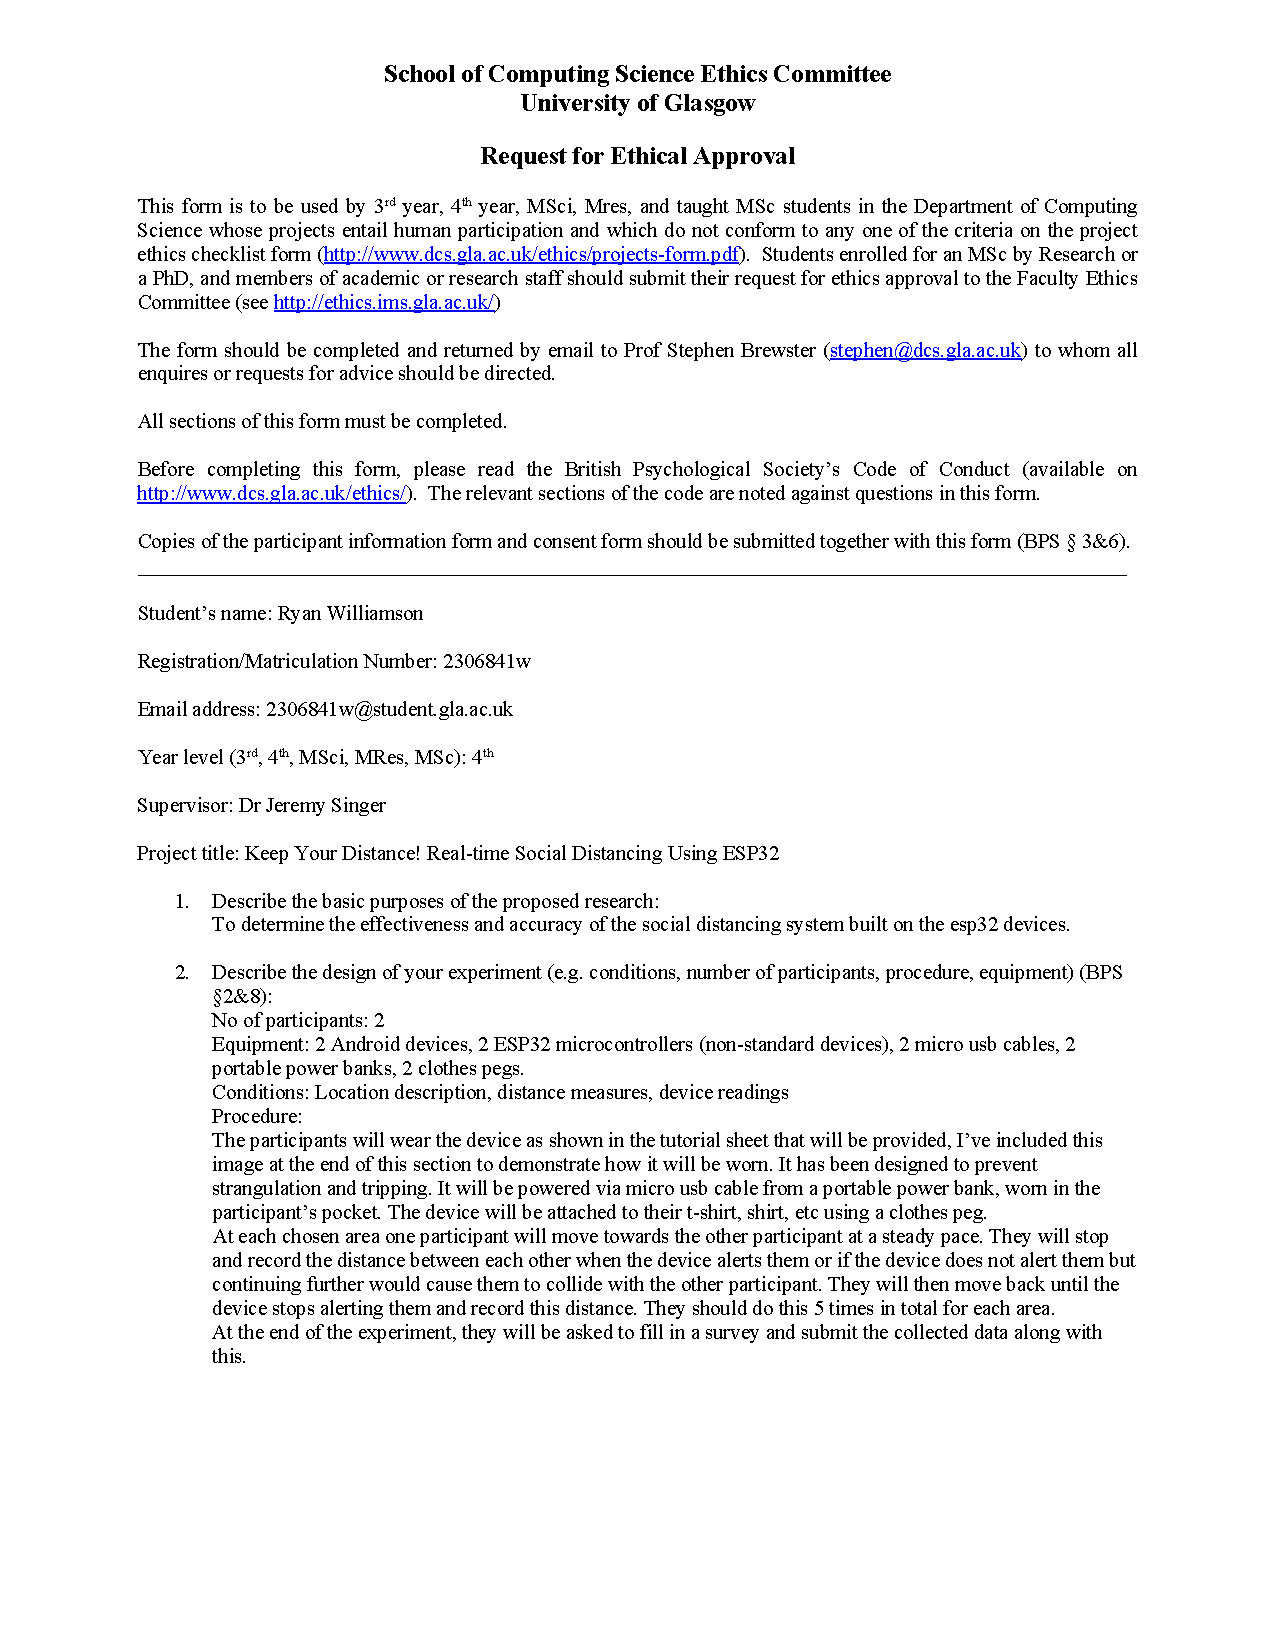
\includegraphics[width=1.0\linewidth]{images/2306841w-ethics-approval 1.pdf}

        \caption{ Signed ethical approval - required for the experiment due to use of non-standard hardware. Part 1 of 3 }

        % use the notation fig:name to cross reference a figure
        \label{fig:full_ethics_approval1}
    \end{figure}

    \begin{figure}[!htb]
        \centering
        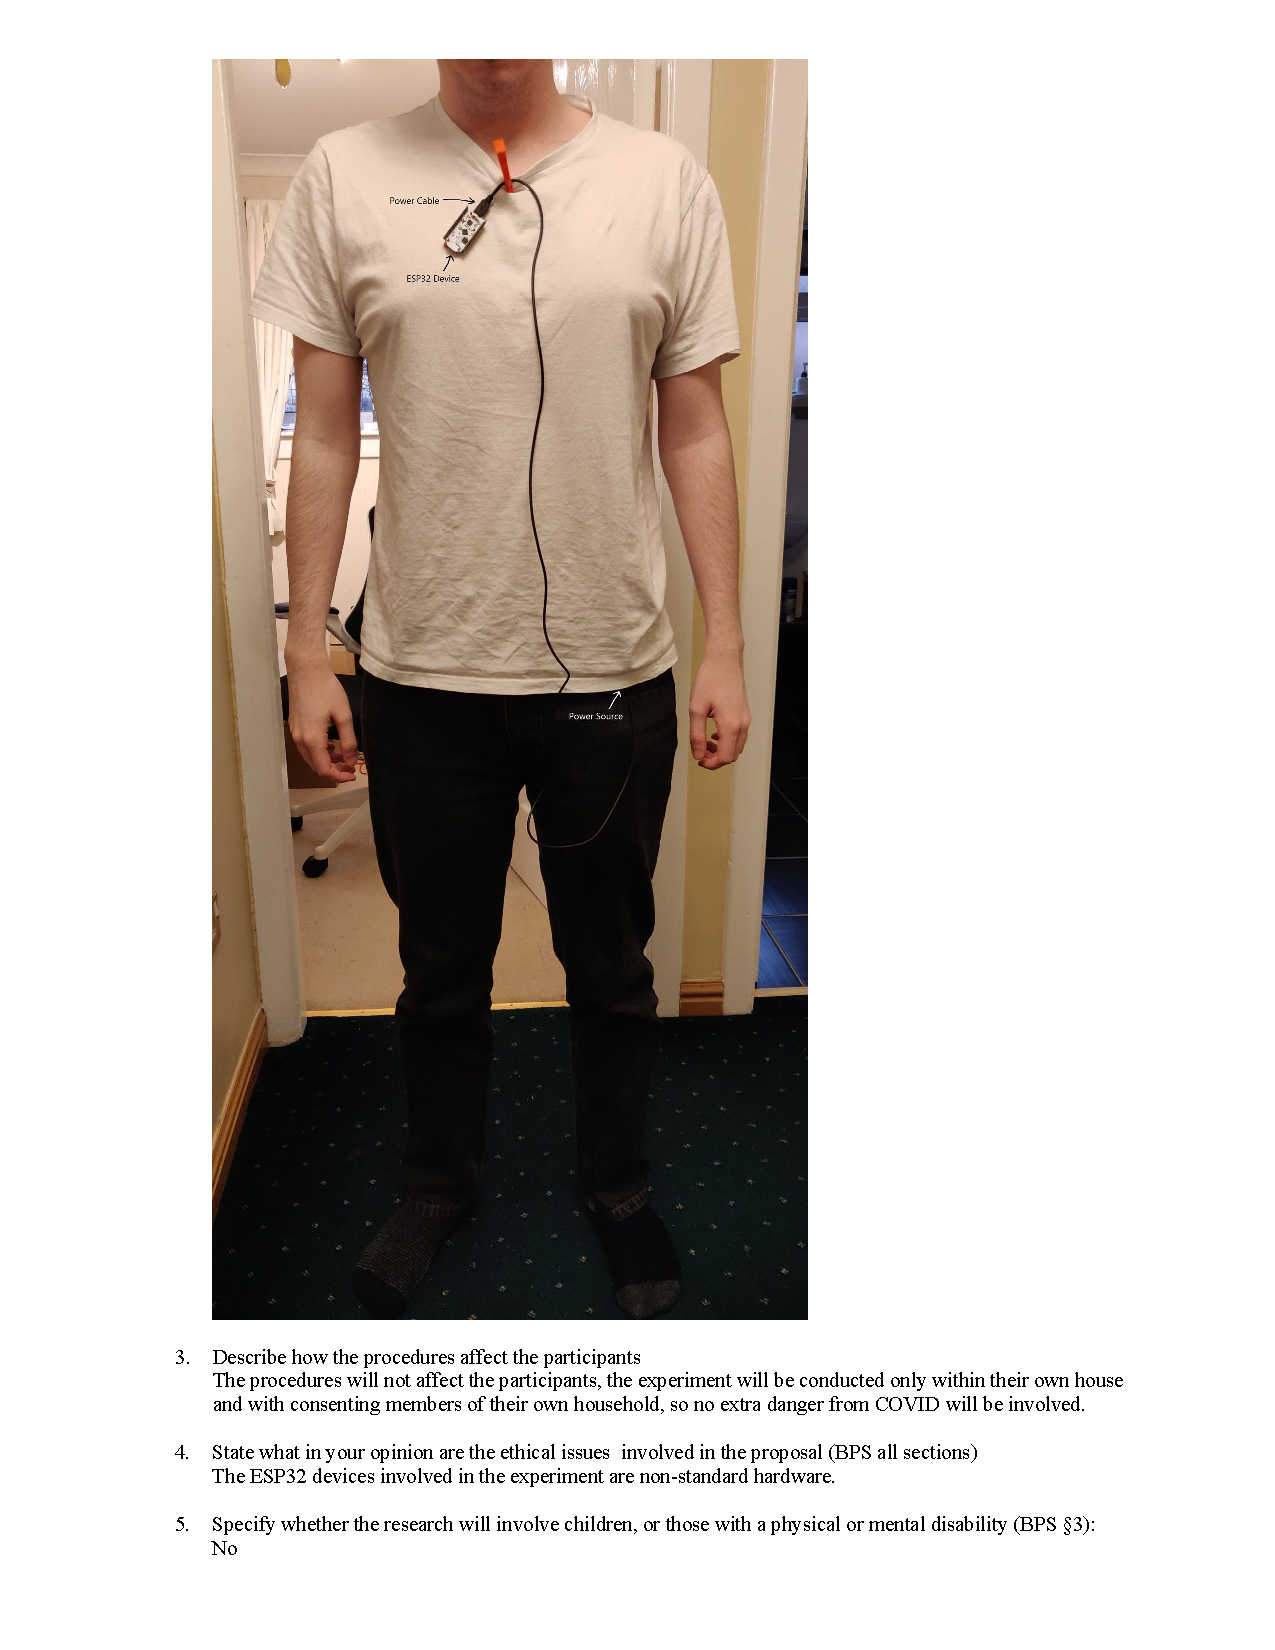
\includegraphics[width=1.0\linewidth]{images/2306841w-ethics-approval 2.pdf}

        \caption{ Signed ethical approval - required for the experiment due to use of non-standard hardware. Part 2 of 3 }

        % use the notation fig:name to cross reference a figure
        \label{fig:full_ethics_approval2}
    \end{figure}

    \begin{figure}[!htb]
        \centering
        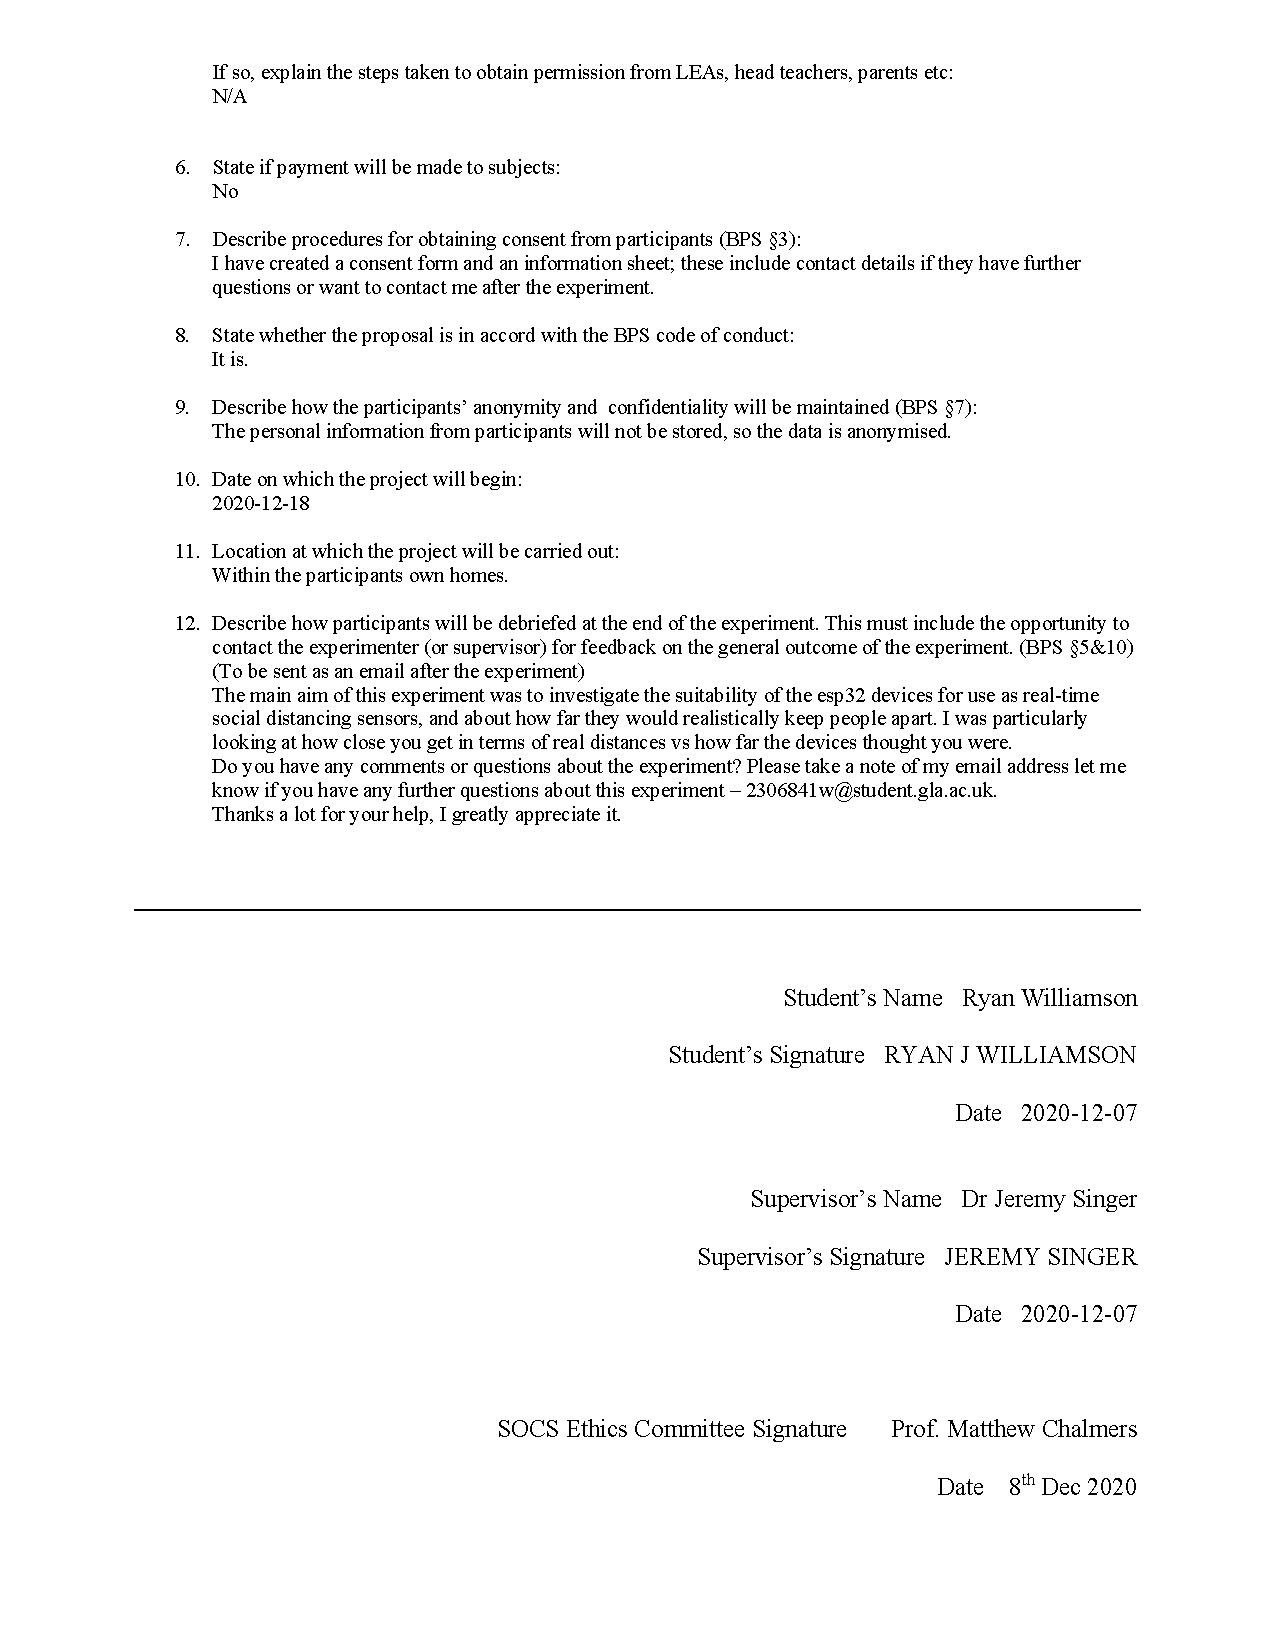
\includegraphics[width=1.0\linewidth]{images/2306841w-ethics-approval 3.pdf}

        \caption{ Signed ethical approval - required for the experiment due to use of non-standard hardware. Part 3 of 3 }

        % use the notation fig:name to cross reference a figure
        \label{fig:full_ethics_approval3}
    \end{figure}

    \begin{figure}[!htb]
        \centering
        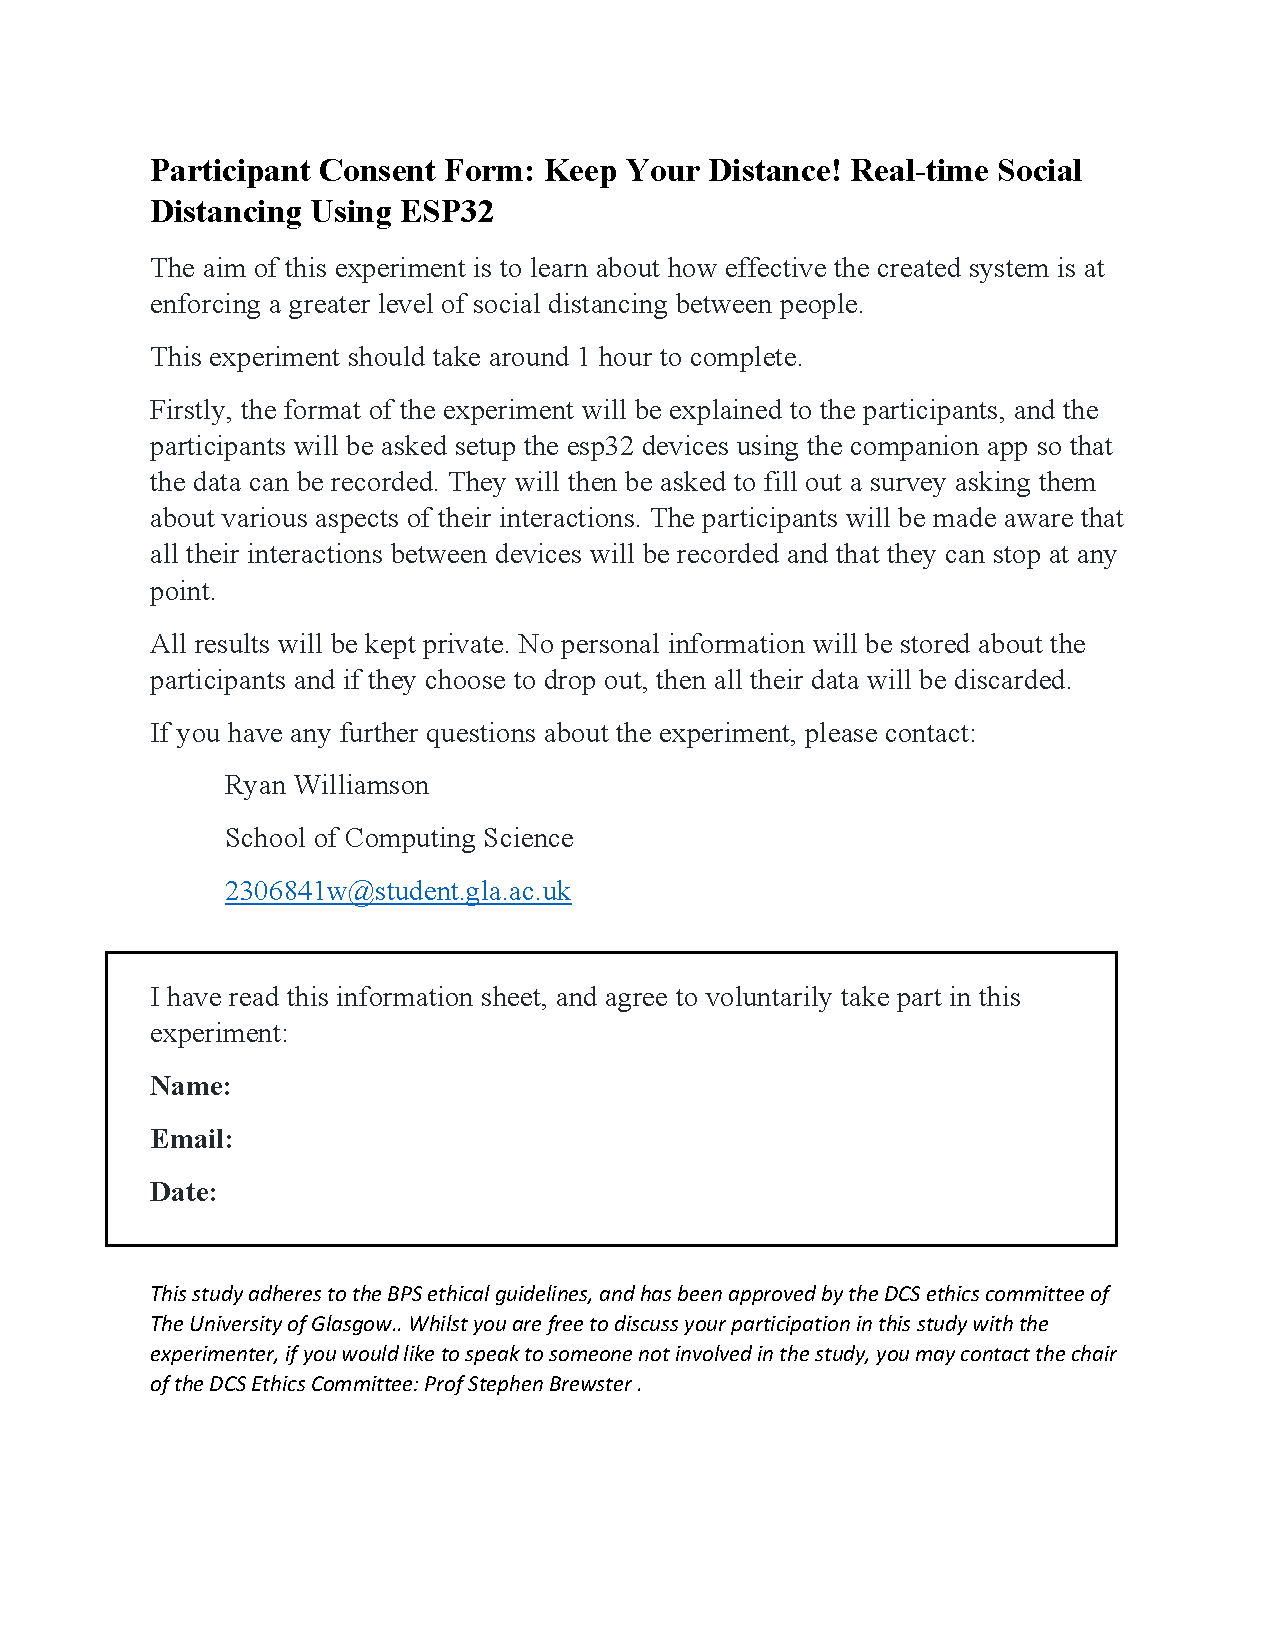
\includegraphics[width=1.0\linewidth]{images/Participant Consent Form.pdf}

        \caption{ Consent form for the experiment. }

        % use the notation fig:name to cross reference a figure
        \label{fig:participant_consent}
    \end{figure}

    \begin{figure}[!htb]
        \centering
        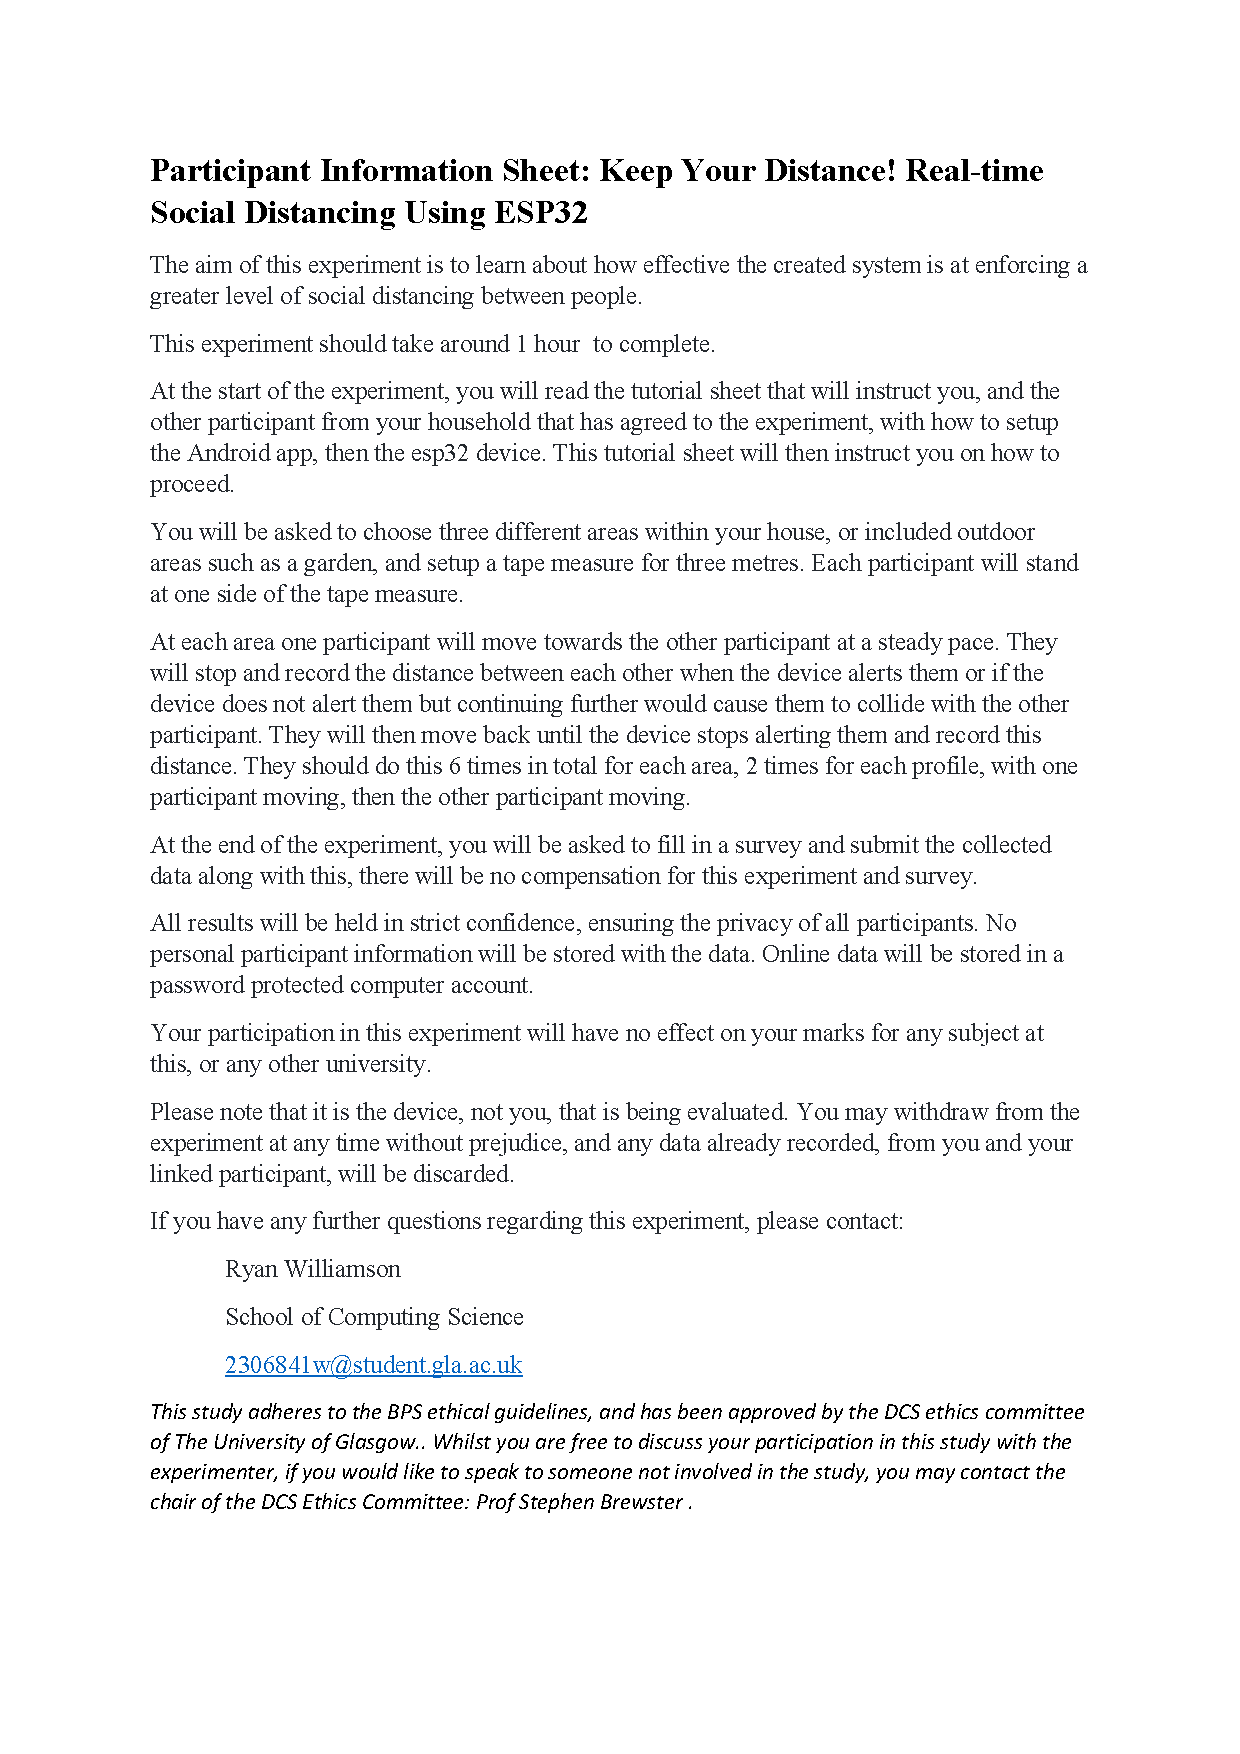
\includegraphics[width=1.0\linewidth]{images/Participant Information Sheet.pdf}

        \caption{ Information sheet, given to the experiment participants before the experiment begins. }

        % use the notation fig:name to cross reference a figure
        \label{fig:participant_information}
    \end{figure}

    \begin{figure}[!htb]
        \centering
        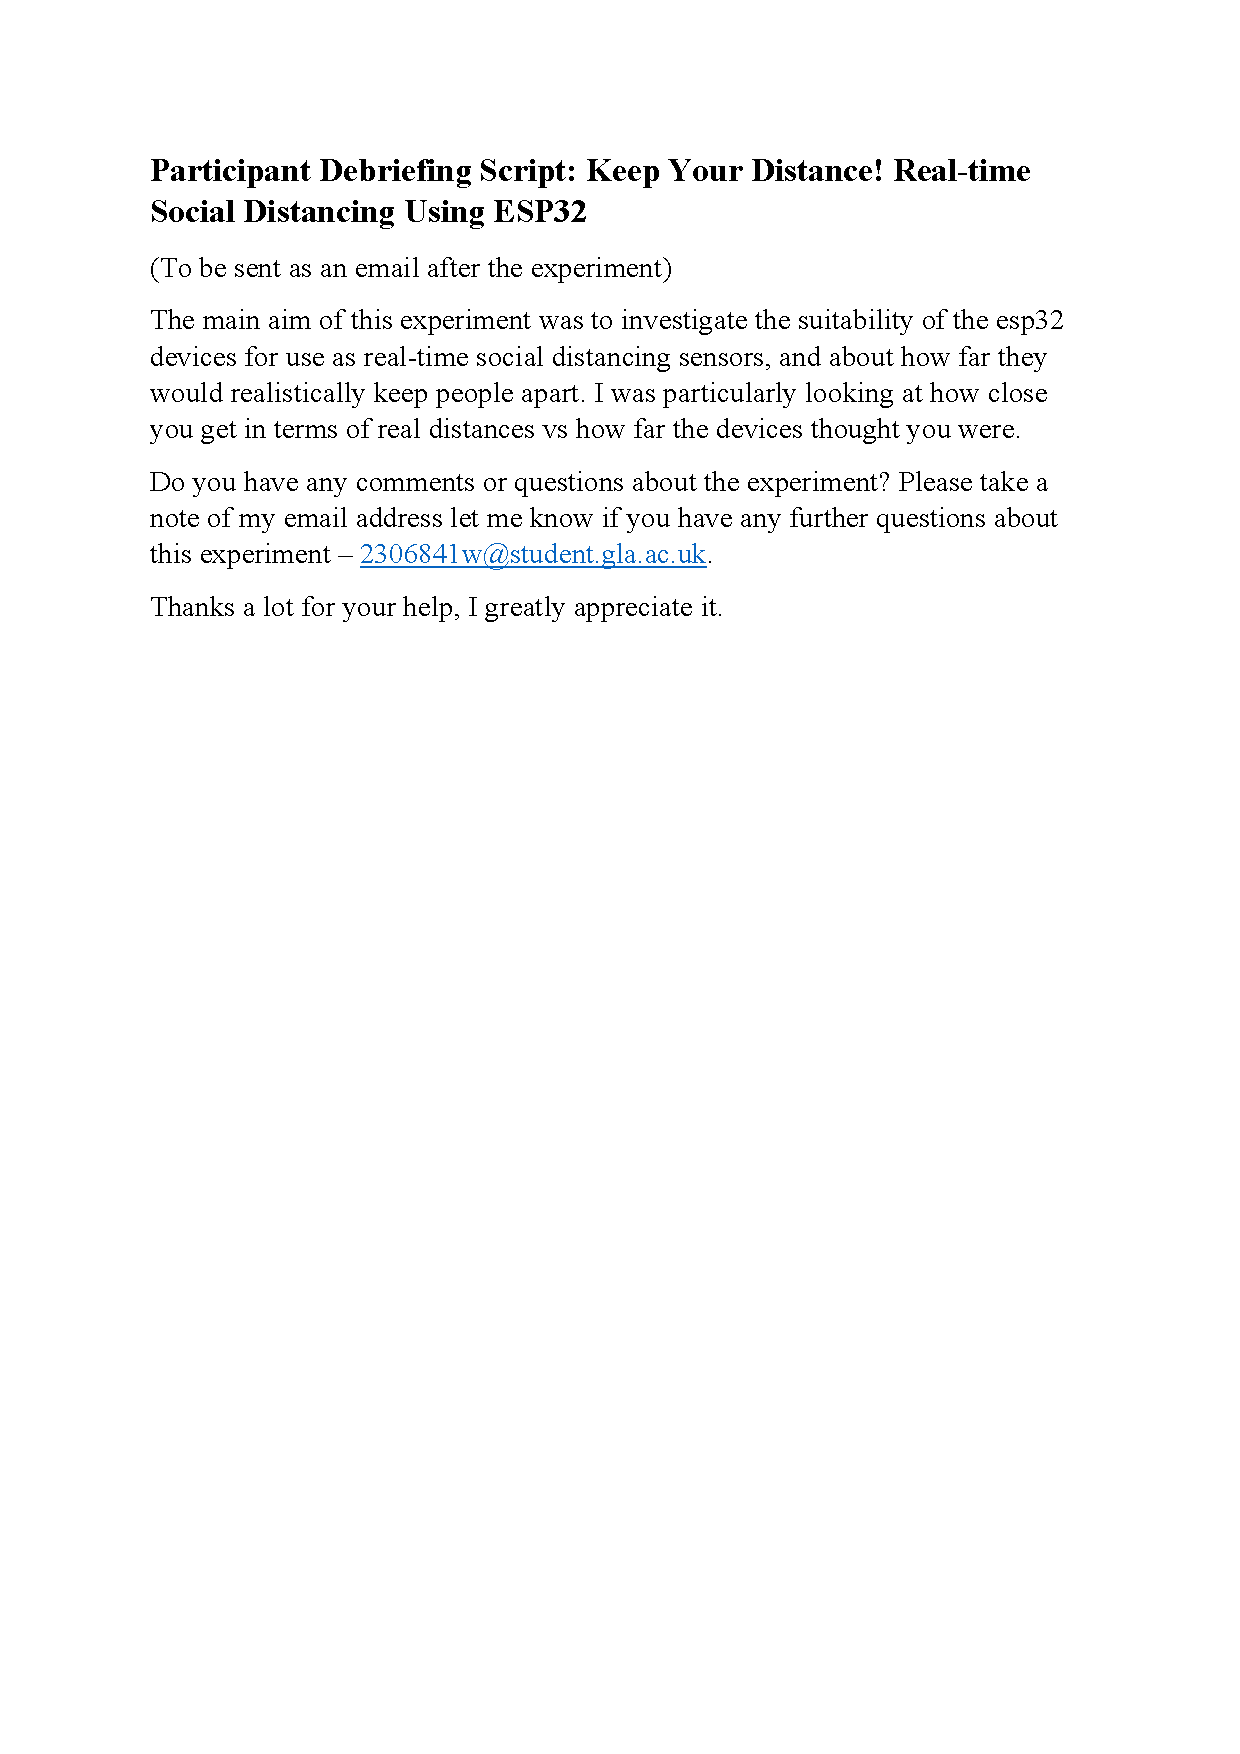
\includegraphics[width=1.0\linewidth]{images/Participant Debriefing Script.pdf}

        \caption{ Debriefing script, given to the experiment participants after the experiment ends. }

        % use the notation fig:name to cross reference a figure
        \label{fig:participant_debriefing}
    \end{figure}

    \chapter{Surveys}

    \begin{figure}[!htb]
        \centering
        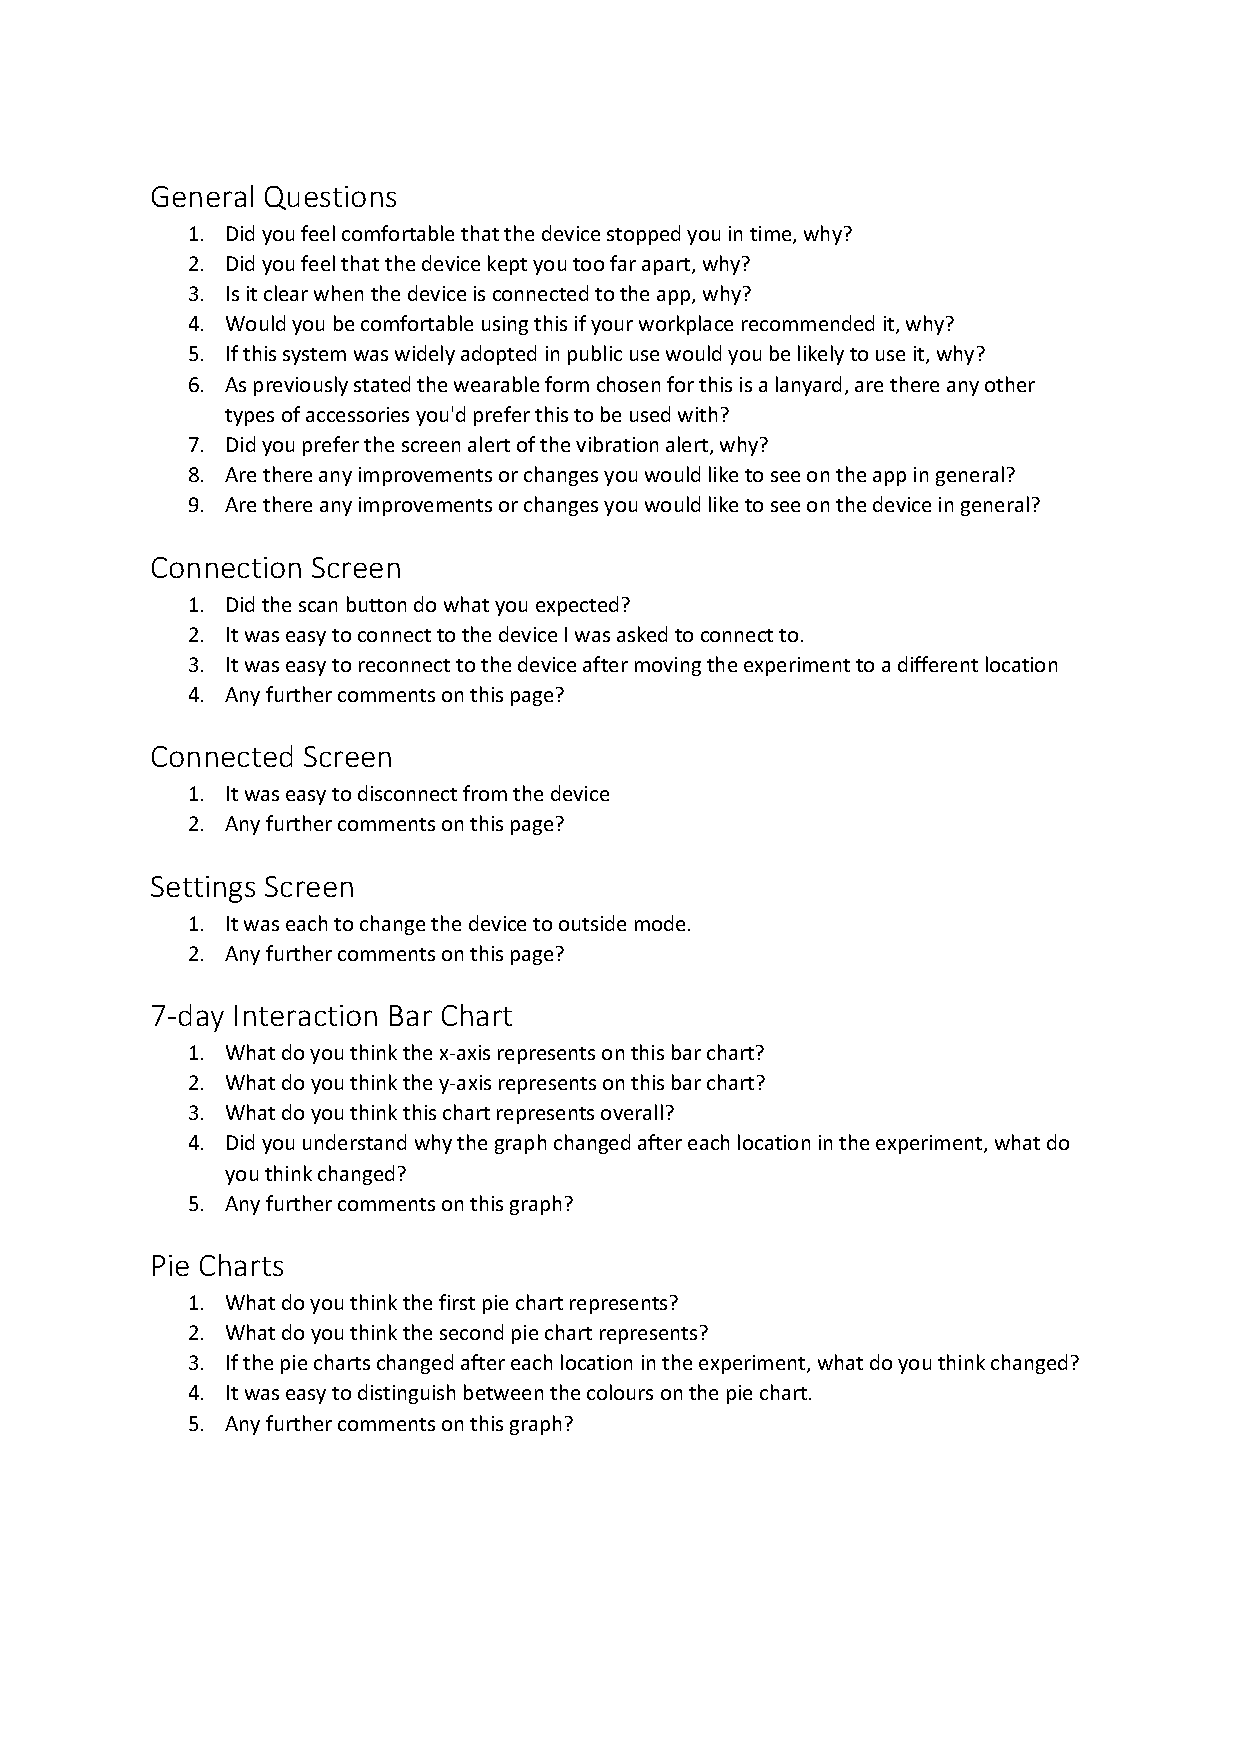
\includegraphics[width=0.85\linewidth]{images/contact-survey_questions 1.pdf}

        \caption{ Survey questions asked after the experiment. Part 1 of 2 }

        % use the notation fig:name to cross reference a figure
        \label{fig:survey-questions-1}
    \end{figure}

    \begin{figure}[!htb]
        \centering
        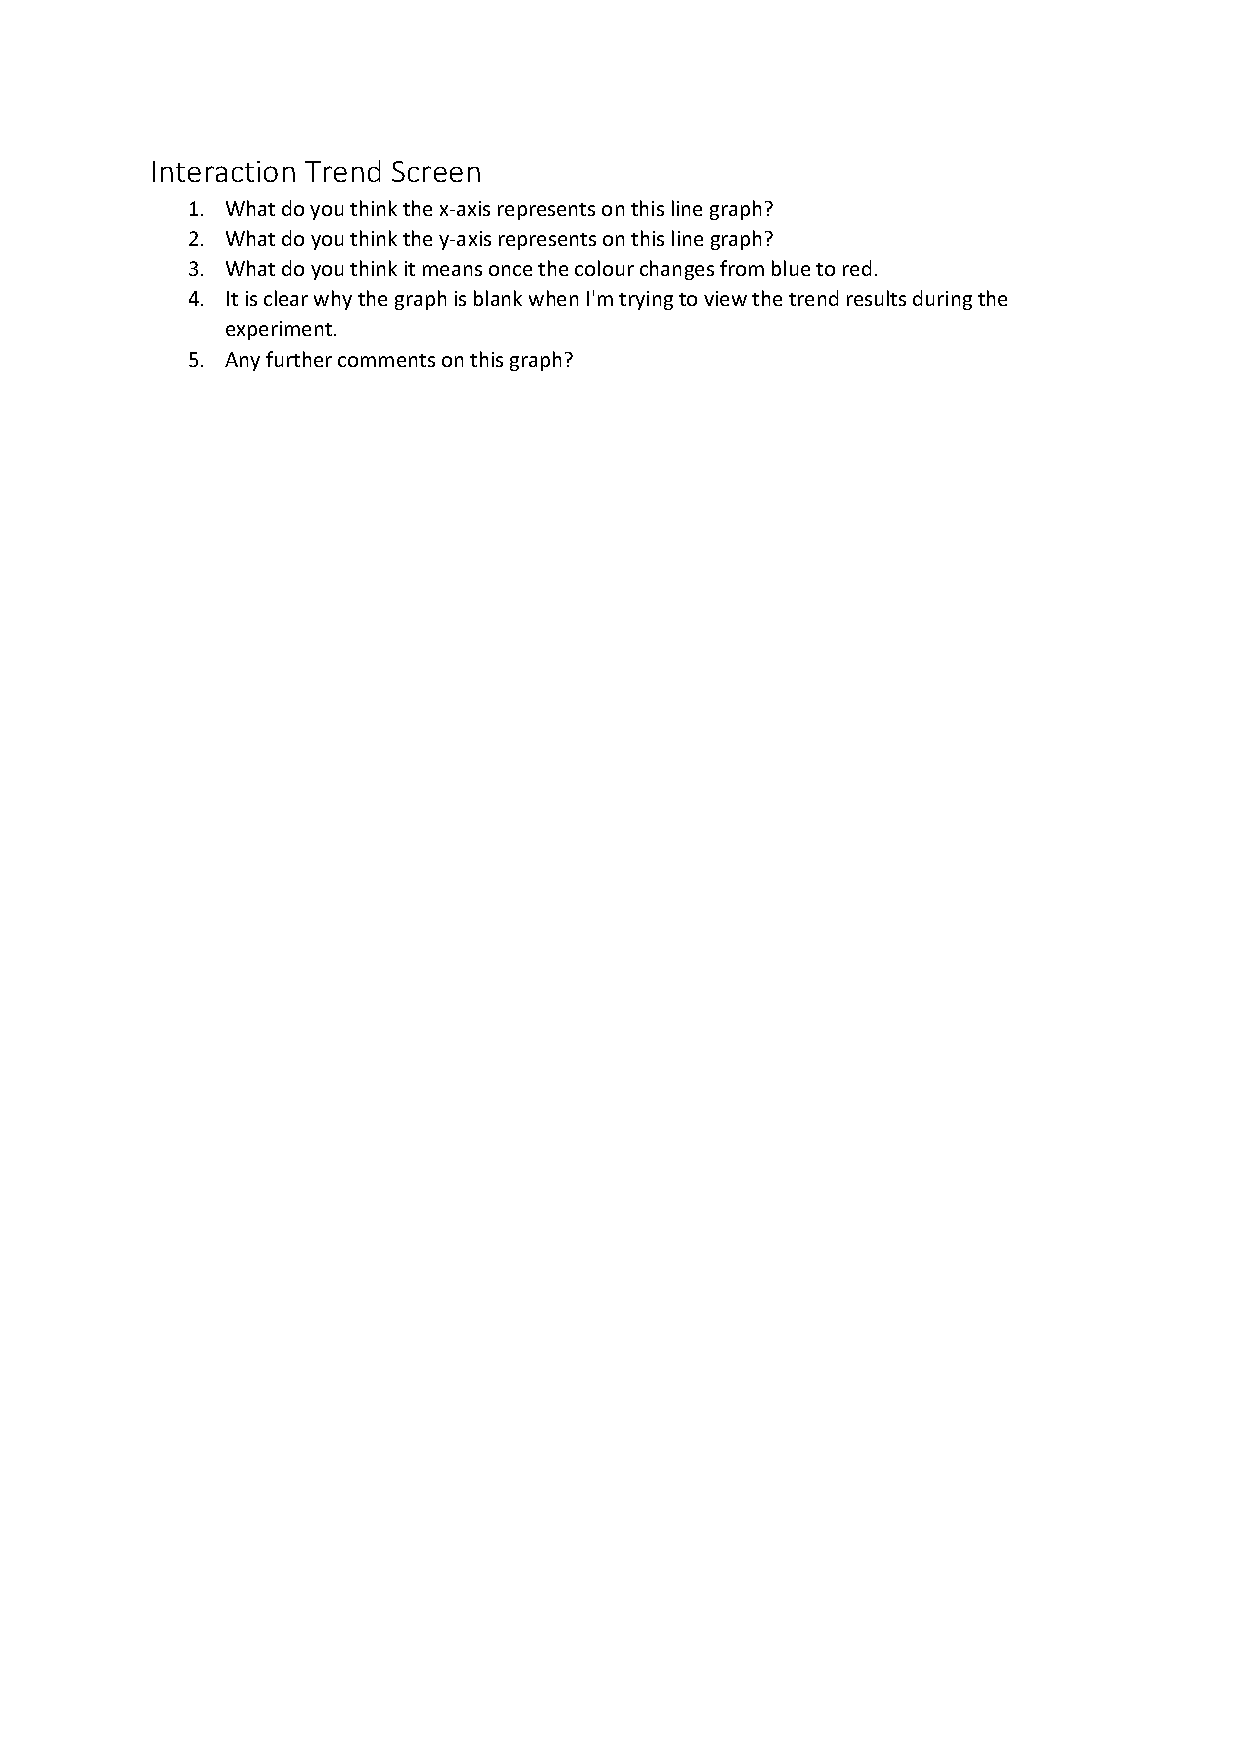
\includegraphics[width=1.0\linewidth]{images/contact-survey_questions 2.pdf}

        \caption{ Survey questions asked after the experiment. Part 2 of 2 }

        % use the notation fig:name to cross reference a figure
        \label{fig:survey-questions-2}
    \end{figure}

    \begin{figure}[!htb]
        \centering
        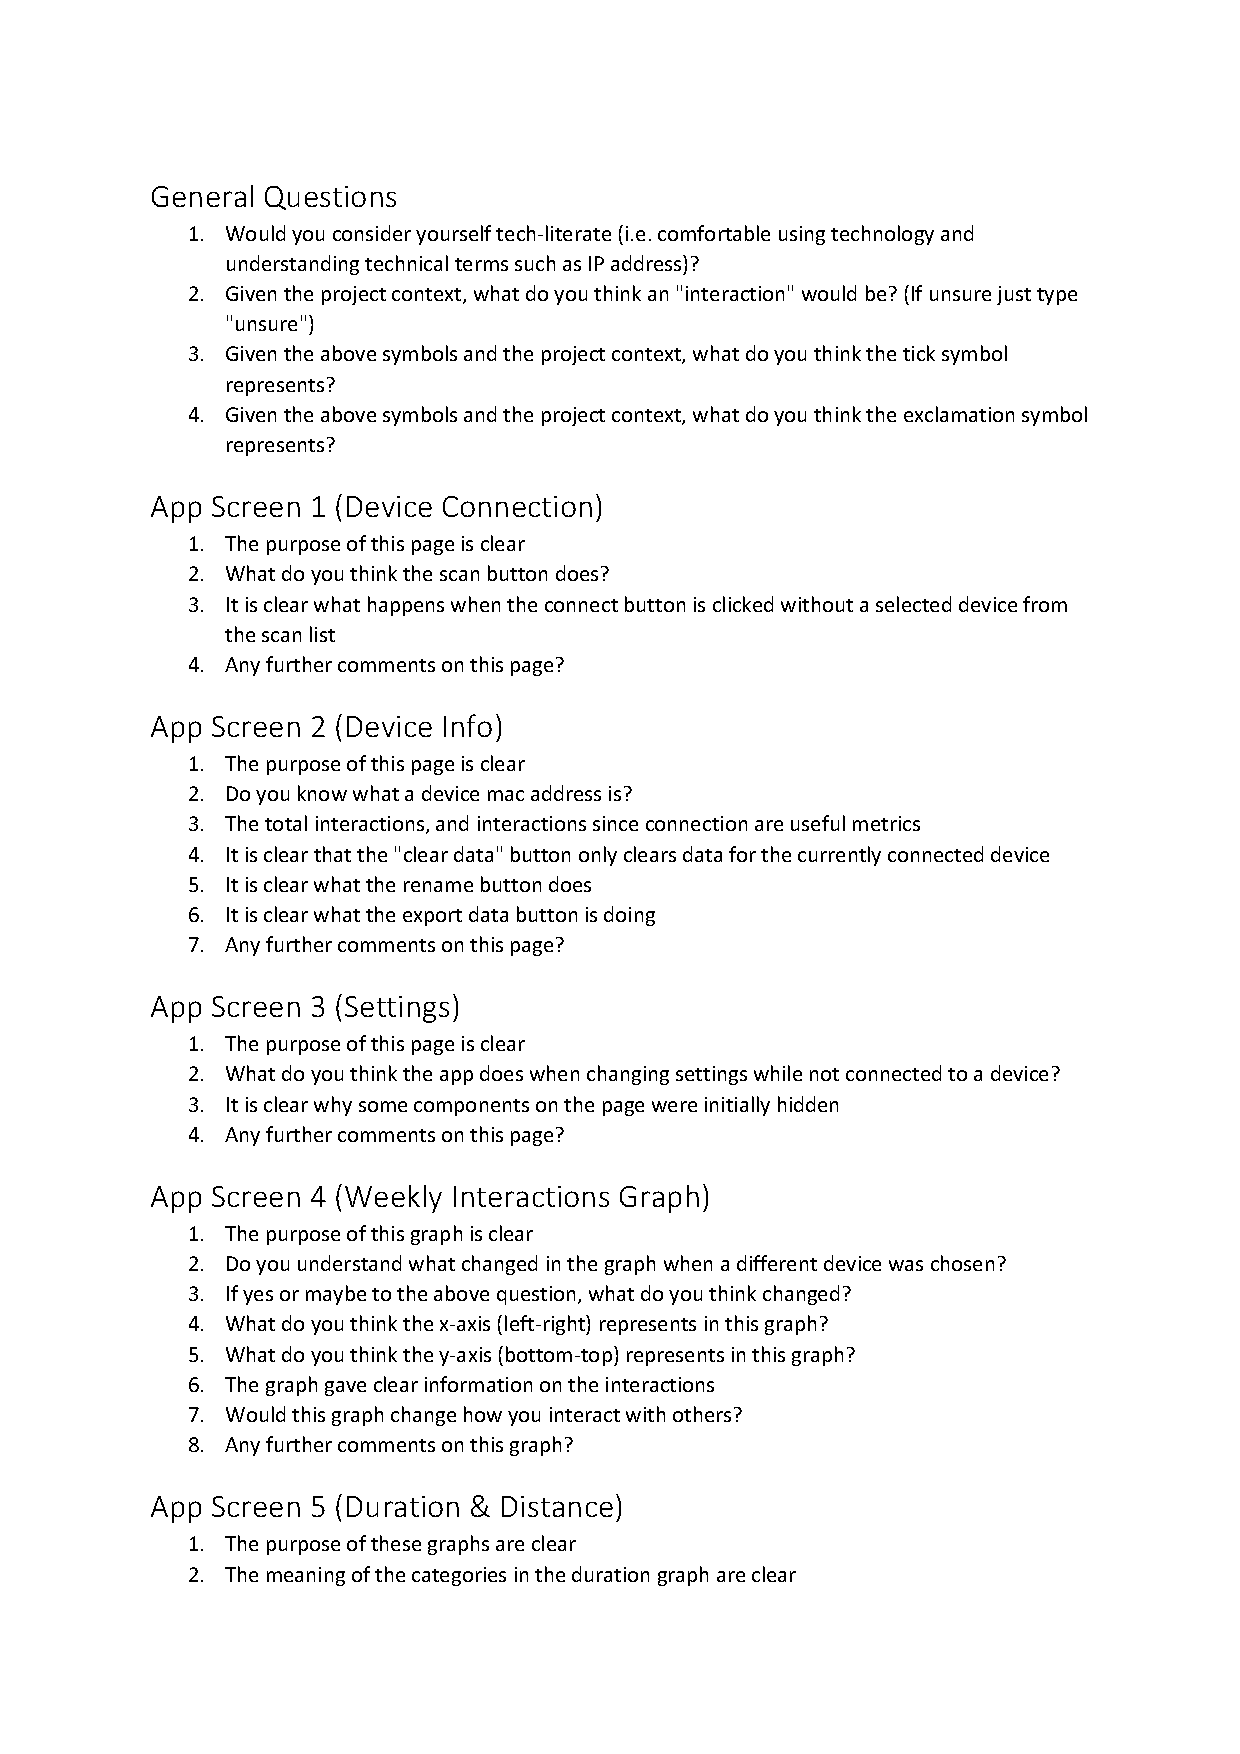
\includegraphics[width=1.0\linewidth]{images/non-contact_survey_questions 1.pdf}

        \caption{ Questions for survey which was sent out for general response. Part 1 of 2 }

        % use the notation fig:name to cross reference a figure
        \label{fig:non-contact-survey-questions-1}
    \end{figure}

    \begin{figure}[!htb]
        \centering
        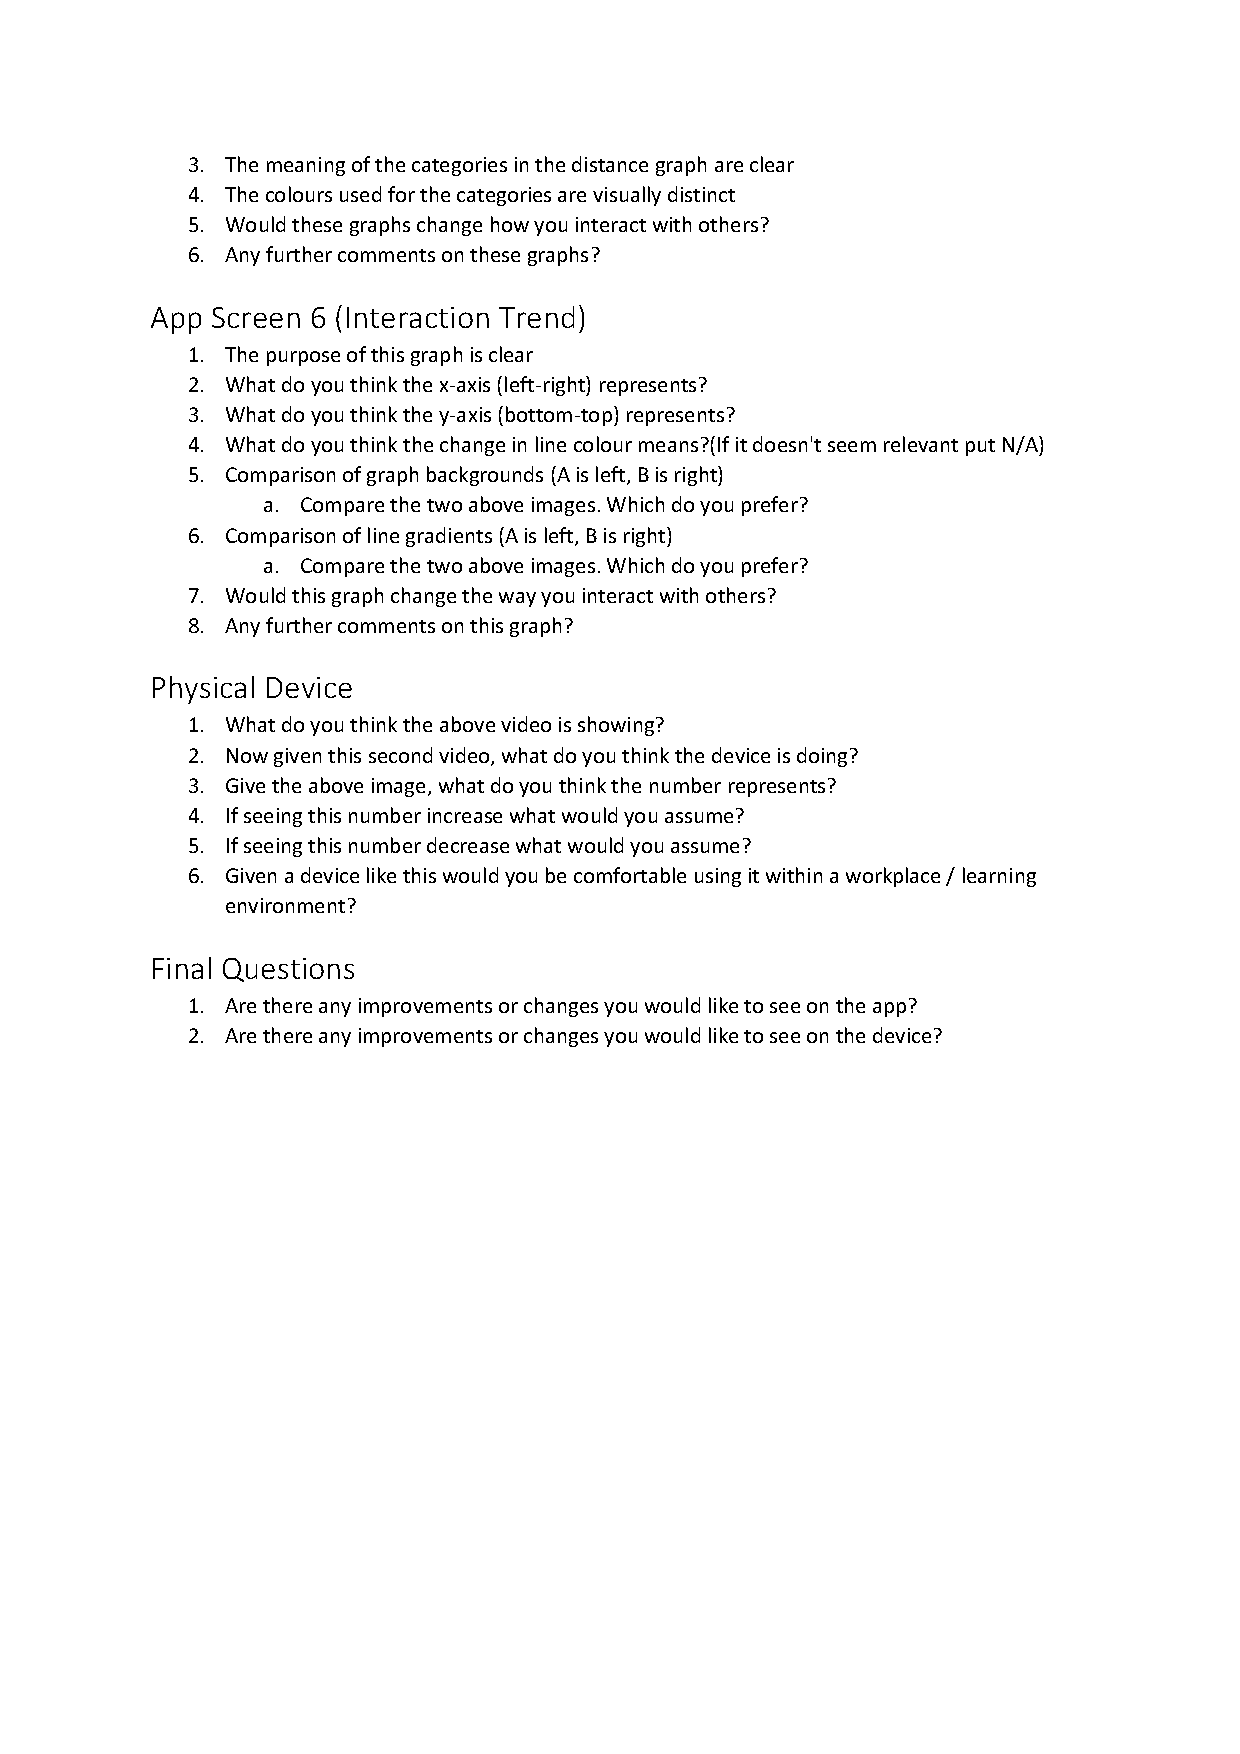
\includegraphics[width=1.0\linewidth]{images/non-contact_survey_questions 2.pdf}

        \caption{ Questions for survey which was sent out for general response. Part 2 of 2 }

        % use the notation fig:name to cross reference a figure
        \label{fig:non-contact-survey-questions-2}
    \end{figure}

    \chapter{Requirements \& Analysis}

    \section{Alex's User Story}

    \begin{figure}[!htb]
        \centering
        \includegraphics[width=1.0\linewidth]{images/user_story.png}

        \caption{ An example user scenario. }

        % use the notation fig:name to cross reference a figure
        \label{fig:alex_user_scenario}
    \end{figure}

\end{appendices}

%==================================================================================================================================
%   BIBLIOGRAPHY   

% The bibliography style is abbrvnat
% The bibliography always appears last, after the appendices.

\bibliographystyle{abbrvnat}

\bibliography{l4proj}

\end{document}
